\documentclass{article}
\usepackage[utf8]{inputenc}

\usepackage[top=2.54cm, bottom=2cm, left=2cm, right=2cm]{geometry}
\usepackage{graphicx}
\usepackage{amsmath}
\usepackage{color}
\usepackage{gensymb}
\usepackage{setspace}
\usepackage{comment}
\usepackage[version=4]{mhchem}
\usepackage{multirow}
\usepackage{amsfonts}
\usepackage{cite}
\usepackage{listings}
\usepackage{xcolor}

\definecolor{lightgray}{rgb}{0.95, 0.95, 0.95}
\definecolor{darkgray}{rgb}{.4,.4,.4}
\definecolor{purple}{rgb}{0.65, 0.12, 0.82}

\lstdefinelanguage{Python}{
    keywords={for, if, in, run, not},
    keywordstyle=\color{blue}\bfseries,
}

\lstset{
    language=Python,
    backgroundcolor=\color{lightgray},
    extendedchars=true,
    basicstyle=\footnotesize\ttfamily,
    showstringspaces=false,
    showspaces=false,
    numbers=left,
    numberstyle=\footnotesize,
    numbersep=9pt,
    tabsize=4,
    breaklines=true,
    showtabs=false,
    captionpos=b
}

\title{\textbf{ATLAS Experiment Shared Laboratory Notebook}}
\author{Daniel Granger (10238277) and Ben Gavan (10301715)}
\date{February/March 2021}

\begin{document}

\maketitle

% \tableofcontents

\section{Notes/Timeline}
\textbf{Conventions:}\\
file names of plots in the format: [Data set]\_[cuts]\_[quantity plotted]\_[energy range]\_[date dd-mm-yy]\_[time (24 hr)].png
\\\\
\textbf{Notes:}
\begin{itemize}
    \item If you want to use a logarithmic scale when plotting a histogram in python then you use canvas.SetLogy(1) or canvas.SetLogx(1) depending on which axis you want to be logarithmic. 'canvas' is your TCanvas object
    
    \item Lead xx == the person programming - other person taking notes in lab book
\end{itemize}
\textbf{ROOT Notes}
\begin{itemize}
    \item lep\_type values:
    \subitem 11 = electrons 
    \subitem 13 = muons
    
    \item Units = MeV
\end{itemize}
\textbf{Acronyms}
\begin{itemize}
    \item MC = Monte Carlo (Simulation)
\end{itemize}

\textbf{Login steps}:
\begin{lstlisting}
ssh atlaslab17@atlaslab17.blackett.manchester.ac.uk

export SINGULARITY_TMPDIR=$HOME/.singularity/tmp

singularity run -B /data/ATLAS:$HOME/ATLAS-Project/ATLAS $HOME/root_6.22.00-conda.sif bash

jupyter-notebook --no-browser --port=8888

New Window:
ssh -N -L localhost:1234:localhost:8888 atlaslab17@atlaslab17.blackett.manchester.ac.uk
\end{lstlisting}

% 2.0273066850004195e-09

\textbf{Spread sheet with cross sections:}
Google sheets in Ben's google drive (Uni/ATLAS/ATLAS)\\ (https://docs.google.com/spreadsheets/d/1ZvxdJ9FcFHIEeIkDnRsDUL7tZVwtQ7-E249czEe7vmM/edit#gid=0)

%%%%%%%%%%%%%% pre-lab %%%%%%%%%%%%%%%% 
%%%%%%%%%%%%%%%% Aims %%%%%%%%%%%%%%%%
\section{Aims}
\begin{itemize}
    \item To gain appreciation of the physics processes that can occur in high energy proton-proton collisions at the LHC
    \item To be introduced to event selection and measurement methods used in particle physics data analysis.
\end{itemize}

%%%%%%%%%%%%%%%% Objectives %%%%%%%%%%%%%%%%
\section{Objectives}
\begin{itemize}
    \item
    \item Compare real data collected by the ATLAS experiment with computer-simulated "Monte Carlo" data.
    \item Measure the cross sections for the production of the Z, W, and Higgs bosons at the LHC and estimate
    statistical and systematic uncertainties of the results.
    \item Gain experience of using \it{ROOT}
    \item Extend the event selections to other sources of events at the LHC, such as:
    \subitem Higgs decaying to two photons
    \subitem events containing tau leptons, pairs of vector bosons, top quarks
    \subitem potential sources of new physics from "Beyond the standard model".
\end{itemize}

%%%%%%%%%%%%%%%% Background Reading %%%%%%%%%%%%%%%%
\section{Background Reading}

\subsection{A femto-course in particle physics}

\subsubsection{Leptons}
Leptons = spin-$\frac{1}{2}$ fundamental particles\\
Charges of $-1, 0, +1$\\
Each generation has a flavour -  electron, muon, tau

\subsubsection{Quarks}
Quarks = spin-$\frac{1}{2}$ fundamental particles\\
Up-type = charge $+\frac{2}{3}$\\
Down-type = charge $-\frac{1}{3}$\\
Bind together via the strong interaction to form Hadrons\\
Baryons = 3 quarks\\
Mesons = quark + anti-quark

\subsubsection{Gauge Bosons}
Responsible for mediating forces

\subsubsection{Higgs Boson}
Does NOT directly mediate a force.\\
It's an excitation of the Higgs field\\
Field gives rise to the masses of the Z \& W bosons. \\

\subsubsection{Parton}
Parton = any constituent of a hadron (q, $\bar{q}$, g)



Main interaction of interest for this experiment = the production \& decay of Z, W and Higgs.\\
Most easily identified decay:
\begin{align}
    Z &\rightarrow l^+ l_-
    \\
    W^- &\rightarrow l^- \bar{\nu}_l
    \\
    H &\rightarrow ZZ^{(*)} \rightarrow llll
\end{align}

%%%%%%%%%%%%%%%% Getting Started %%%%%%%%%%%%%%%%
\section{Getting Started}
Start a Jupyter notebook server running on the lab machine.
Can then connect to this server using a web browser from anywhere.

\subsection{Logging into the Lab machine}
\begin{enumerate}
    \item Open terminal
    \item \it{ssh atlaslab[lab machine \#]@atlaslab[lab machine \#].blackett.manchester.ac.uk}
    \item Answer yes
    \item Enter the password for the specific machine
\end{enumerate}

\subsection{Setting up the code - TODO once at the start of the experiment}\label{subsec:setting-up-the-code}
A skeleton version of the code is providied.\\
To work in python: \textit{cp -r /opt/ATLAS-Project-py ATLAS-Project}\\
Then type in:\\
\begin{itemize}
    \item \textit{cd ATLAS-Project}
    \item \textit{mkdir outputPlots}
    \item \textit{ls -l}
\end{itemize}
Can then log out using \textit{exit}

\subsection{Starting up the Jupyter notebook server}
Need to be followed at the beginning of each lab day.\\
Uses Singularity to run a Jupyter notebook server on the lab machine.
\begin{enumerate}
    \item Log into the lab machine using~\ref{subsec:setting-up-the-code}

    \item Configure Singularity
    \\\\
    \textbf{export SINGULARITY\_TMPDIR=\$HOME\/.singularity/tmp} - sets up the scratch directory
    \\
    \textbf{singularity run -B /data/ATLAS:\$HOME/ATLAS-Project/ATLAS \$HOME/root\_6.22.00-conda.sif bash}
    \\\\
    Should see \textbf{INFO: Convert SIF file to sandbox...} and then after about a minute \textbf{Singularity$>$}

    \item Start the Jupyter Notebook
    \\\\
    \textbf{jupyter-notebook --no-browser --port=8888}
    
    \item Should expect text that looks like:
    \\\\
    \textit{Writing notebook server cookie secret to /home/atlaslab16/.local/share/jupyter/runtime/notebook cookie secret
    Loading IPython parallel extension
    Serving notebooks from local directory: /home/atlaslab16
    The Jupyter Notebook is running at: http://localhost:8888/?token=a7ea520d2f4d6f62ea2026ac0aa1edd0a48e935b03539bc4 or http://127.0.0.1:8888/?token=a7ea520d2f4d6f62ea2026ac0aa1edd0a48e935b03539bc4 Use Control-C to stop this server and shut down all kernels (twice to skip confirmation).
    .
    To access the notebook, open this file in a browser: file:///home/atlaslab16/.local/share/jupyter/runtime/nbserver-15700-open.html Or copy and paste one of these URLs: http://localhost:8888/?token=a7ea520d2f4d6f62ea2026ac0aa1edd0a48e935b03539bc4 or http://127.0.0.1:8888/?token=a7ea520d2f4d6f62ea2026ac0aa1edd0a48e935b03539bc4}
    \\\\
    Need to keep this terminal window open.
    
    \item Open another terminal window:
    \\\\
    \textbf{ssh -N -L localhost:1234:localhost:8888 atlaslab[MACHINE NUMBER]@atlaslab[MACHINE NUMBER].blackett.manchester.ac.uk}

    \item Enter the machine password  \\
    Also keep this terminal window open.

    \item Use any browser to connect to 
    \\\\
    \textbf{localhost:1234}

    \item Should be presented with a Jupyter page asking for a \textbf{token} to be entered at the top of the page in the \textbf{token or password} box.

    \item Use the token given in the terminal window from a couple of steps ago.
\end{enumerate}

\subsection{Closing the Jupyter Notebook and Logging out of the lab machine}
\begin{enumerate}
    \item \textbf{ctrl+C} on both terminal windows.
    \item then enter
    \\\\
    \textbf{y} | Close down the Jupyter notebook server\\
    \textbf{exit} | Closes Singularity\\
    \textbf{exit} | Logs out from the lab machine.
\end{enumerate}

\subsection{Using Analysis.py}
Add names and date to the top of \textbf{Analysis.py} in a comment.\\
\textbf{lep\_n}: Int = Number of leptons identified in each event.\\
\textbf{lep\_pt}: Vect = vector of the lepton momenta in the plane transverse (perpendicular) to the beam direction (the z coordinate points along the beam).\\
All available data sets: \url{http://opendata.atlas.cern/release/2020/documentation/datasets/dataset13.html}\\\\
Values of energies and momenta are given in units of \textbf{MeV}.

\subsection{Running the Skeleton code and examining the produced kistograms}
Page 13 (14) for Monte Carlo data sets with string code.  (String code = What is typed in Run-Analysis.py)\\
Full list ccan be found in the file \textbf{backend/dataSets.py}\\
\\
Remember to select \textit{Save and Checkpoint} from \textit{File} drop-down.
Can then \textit{Revert to Checkpoint} from \textit{File} drop-down.
\\\\
The file \textit{Analysis.py} contains a single function, \textit{Analyse}.
It is called once per data set analysed.
In this function, will:
\begin{itemize}
    \item select events
    \item plot histograms
    \item set histogram styles
    \item write plotted histograms to an output file.
\end{itemize}

%%%%%%%%%%%%%%%% Analysis %%%%%%%%%%%%%%%%
\section{Analysis}

Selection cut to select a sample of events corresponding to the desired particular physics processes.\\
There is a trade off  between  the conflicting aims of achieving as high as possible a selection efficiency for the signal and rejecting as much as possible of the "background" from other physics processed.\\
It's more important to make estimates of the selection efficiency and the level of residual background.
And to come up with credible statistical and systematic uncertainties on these estimates.
\\\\
Note that the generated particles are not always actually observed in  the ATLAS detector.\\
Note that the events may contain additional particles (e.g. jets of hadrons produced by radiation from the incoming partons before the annihilation that produced the Z boson)

\subsection{Analysing Z bosons}

ATLAS uses a right-handed coordinate system.
Origin at the nominal interaction point in the centre of the detector and the z-axis along the beam pipe.
The x-axis points from the interaction point to the centre of the LHC ring.
y-axis upwards.
\\\\
In the data, the kinematic variables given for each lepton are:
\begin{itemize}
    \item transverse (perpendicular) momentum - $p_T$
    \item azimuthal angle $\phi$ between $p_T$ and the x-axis
    \item pseudorapidity $\eta$
\end{itemize}
Pseudorapitdity is a spatial coordinate describing the angle of a particle relative to the beam axis defined as
\begin{align}
    \eta = -ln \left( \tan\left( \frac{\theta}{2} \right) \right)
\end{align}
where $theta$ = the polar angle\\
When high (small angle) the parricle is usually along the beam exis (often lost)
For massless particles, this is equivalent to the rapidity ($y$) defined as
\begin{align}
    y = \frac{1}{2}  \ln \left( \frac{|\vec{p}| + p_L}{|\vec{p}| - p_L} \right)
\end{align}
where $p_L$ is the longitudinal momentum and $\vec{p}$ is  the 3-momentum of the particle.

%    TODO: Exercise: Derive a conversion from the kinematic  variable set $(p_T, \phi, \eta)$ to $p_x, p_y, p_z$

\subsubsection{Excercise 6.2}
Derive an expression for $m_{ll}$ for the decay $Z \rightarrow \mu^+ \mu^-$
\\\\
The invarient mass of the system can be expressed directly using....
\begin{align}
    m_{ll}^2 = 2 p_{T1} p_{T2} \left( \cosh (\eta_1 - \eta_2) - \cos(\phi_1 - \phi_2) \right)
\end{align}

\subsection{Making event selction cuts}
Selection criteria/cuts on each event - e.g. only interested in events with oppositely charged leptons of the same type/flavour.
\\
Can restrict the events plotted by using the $p_T$ of the leptons.
In general, always want to use the  particles with the highest $p_T$.

\subsubsection{Exercise 6.6}
%    TODO: Find the invariant mass of Z \rightarrow on the MC data set and the 2lep data set


Leptons produced in the decay of Z and W bosons tend to be "isolated" from other particles produced in p-p collisions.
\\
Leptons from "background" processes (e.g. decay of b quarks) tend to be accompanied by a jet of other particles.

\subsubsection{The Isolation Variables - ptcone30 and etcone20}
\textit{ptcone30} (ntuple)  = a sum over the $p_T$ of all tracks contained within a cone of half-width 0.3 in $\delta R$ around the lepton direction
\begin{align}
    \Delta R = \sqrt{\Delta \phi^2 0}
\end{align}
\textit{etcone20} (ntuple) = contains a sum over the $p_T$ cone


\subsection{Event weights for Monte Carlo data sets}
The used ATLAS datasets correspond to an "integrated luminosity" $\int L dt$ = $10.064 \text{fb}^{-1}$ ("inverse femtobarns").
= a measure of the number of the p=p collisions in ATLAS.
\\
The Monte Carlo
\\\\
Integral corresponds to the sum of all weights for all the calls of \textit{Fill} for which the plotted value lies between the lower and upper bounds of the histogram.
It is \textit{Intergral} that should be compared NOT \textit{Entries} (when comparing histograms of ATLAS and MC data).


\subsection{Cross Sections, backgrounds, and efficiencies}
Cross section $\sigma$ for a given process such as $Z \rightarrow ll$:
\begin{align}
    \sigma (pp \rightarrow Z \rightarrow ll) &= \frac{N^{selected} -  N^{background}}{\epsilon \int L dt}
    \\\\
    N^{\text{selected}} &= \text{ total number of events in the ATLAS data that pass the final selection cuts}
    \\
    N^{\text{background}} &= \text{ estimate of the number of background events in the selected data sample}
    \\
    N^{selected} -  N^{background} &= \text{estimate of the number of "signal" events in the ATLAS data for the targeted physics process}
%        \\
%        \epsilon &= \text{ efficiency for selecting the "signal" events. "signal" = whichever physics process that is having its cross section being measured.\\
%        Can be estimated using MC for the target sample process. \\
%        The sum of weights for all signal MC  events that pass the selection cuts needs to be divided by  that corresponding to all generated events for the relevant sample.\\
%        Info provided by running \textit{TotExpected.py}}
\end{align}
To get the sum of weights for all generated $Z \rightarrow ll$ signal MC events:
\begin{align}
    & \text{\textbf{python3.4 TotExpected.py}}
    \\
    & \text{\textbf{Zee}}
\end{align}

Fractional uncertainty on $\int L dt$ = 1.7\%

Other systematic uncertainties may arise, for example, from:
\begin{itemize}
    \item backgrounds not accounted for
    \item disagreements between simulation and real data
\end{itemize}
Possible catch all to estimate the size of such effects = to re-calculate the cross section having changed your event selection cuts

\subsection{Re-discovering the Higgs boson}
Simplest Higgs decay mode:
\begin{align}
    H \rightarrow ZZ^{(*)} \rightarrow llll
\end{align}
 - Look at events producing 4 leptons\\
 - 2 same-flavour, opposite-charge pairs.




%%%%%%%%%%%%%% 09/02/2020 %%%%%%%%%%%%%%%% 
%! Author = ben
%! Date = 09/02/2021

\subsection{Aims}
\begin{itemize}
    \item Establish Connection
    \item Set up Jupyter Notebook
    \item
\end{itemize}

\subsection{Day Summary}

\subsubsection*{09:00}
Create shared overleaf document to share plots and lab notes:
\\
\textit{https://www.overleaf.com/project/60251ee135265fbc62f06417}
\\
\textbf{Exercise 6.1:}
\\
Derive a conversion from the kinematic variable set $(p_T, \phi, \eta)$ to $(p_x, p_y, p_z)$
\begin{align}
    \dots
\end{align}
\textbf{Exercise 6.2:}\\
Derive an expression for $m_{ll}$ for the the decay $Z \rightarrow \mu^+ \mu^-$.
\begin{align}
    \dots
\end{align}
\\\\
\textit{http://opendata.atlas.cern/release/2020/documentation/datasets/dataset13.html}

\subsubsection*{\textbf{9:20} - Lead DG}
Logging onto manchine 3.

\subsubsection*{\textbf{9:30}}
Set up Jupyter notebook on lab machine 3, Password: Atlasfp423.

\subsubsection*{\textbf{10:00} - Lead BG}

\subsubsection*{\textbf{10:07}}
Issue in 5.2: access denied when specifying language

\subsubsection*{\textbf{10:24}}
Resolved: There was a temporary conflict on the machine

\subsubsection*{\textbf{11:42}}
Issue in 5.3 (3\&4): Token not provided, Tried on both computers- still no change.

\subsubsection*{\textbf{12:14}}
Issue in 5.3(7): Incorrect page in web browser (Only shows password).
\\
Resolved: New machine used (mu=3) (changed to mu=17).

ssh string:
\begin{lstlisting}
ssh -N -L localhost:1234:localhost:8888 atlaslab17@atlaslab17.blackett.manchester.
ac.uk
\end{lstlisting}

\subsubsection*{\textbf{14:00} - Lead: DG}

\subsubsection*{\textbf{15:00} - Lead: BG}

\subsubsection*{\textbf{16:00}}
Exploring Analysis.py and LabNotebook.ipynb

\subsubsection*{\textbf{17:00}}
Log off for the day.

%%%%%%%%%%%%%% 11/02/2020 %%%%%%%%%%%%%%%% 
\newpage
%%%%%%%%%%%%%% 11/02/2020 %%%%%%%%%%%%%%%% 
\subsection*{\textbf{11/02/2020}}

\subsection{Aims}
\begin{itemize}
    \item Completed Exercise 6.4
    \subitem Invariant mass of 2 lepton system
    \item Complete Exercise 6.7
    \subitem etcone20
    \subitem ptcone30
\end{itemize}

\subsubsection{Day Summary}
\begin{itemize}
    \item Completed Exercise 6.4
    \subitem Invariant mass using Zmumu MC
    \subitem Invariant mass using 2lep (lep-n==2)
    \subitem Invariant mass using 2lep (lep-n==2 \&\& lep-type==13) (11 = e, 13 = mu)
    \subitem 
    \item Completed Exercise 6.7
    \subitem plot graphs of ptcone30 and etcone20
    \item Plotted the invariant mass using 2lep (ATLAS) data for:
    \subitem ee lepton pair 
    \subitem $\mu\mu$ lepton pair
    \subitem $\tau\tau$ lepton pair
\end{itemize}

\subsubsection*{\textbf{09:20} - Lead DG - Exercise 6.4}
(Exercise 6.4) Plotting the invariant mass using Zmumu MC data
\\
Error in “Analysis.py” - null pointer “ hinvmassZll.Write()”
Remove all unnecessary code
\\
https://www.overleaf.com/project/60251ee135265fbc62f06417

\subsubsection*{\textbf{10:56}}
Narrowed error down to “.setAlias” string

\subsubsection*{\textbf{11:00}}
Error Found:  missing bracket and not using lowercase functions.
\\
Success at plotting the sum of pT (transverse momenta) of the Z boson using MC $Z \rightarrow ll$ data.


\subsubsection*{\textbf{11:12}}
Success plotting the invariant mass of the Z boson using MC (fast mode) for $Z \rightarrow \mu\mu$: figure.\ref{fig:zll_inv-mass_50-150GeV_11-02-21_11:12}
\\
From MC:\\
Mean: (9.018±0.766)e+4 MeV \\
Expected: (9.1187±0.00021)e+4 MeV\\
Cuts used Fig.\ref{fig:zll_inv-mass_50-150GeV_11-02-21_11:12}:
\begin{itemize}
    \item lep-n == 2
\end{itemize}
 
\begin{figure}[h!]
    \centering
	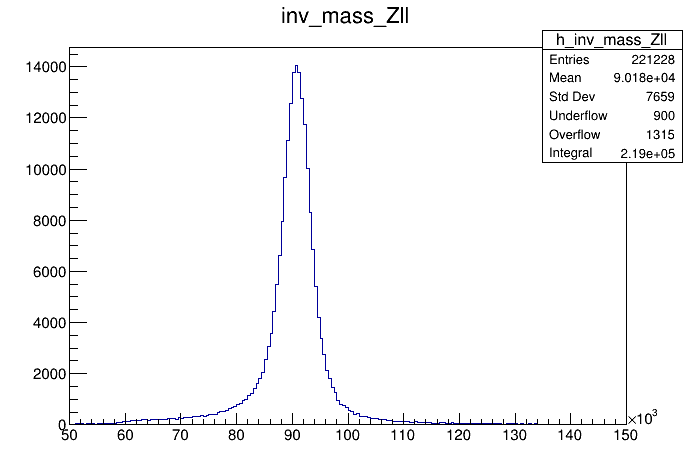
\includegraphics[width=0.85\linewidth]{plots/11-02-2021/Zll-fast_inv-mass_50-150GeV_11-02-21_11:12.png}
	\caption{(Exercise 6.4) (Fast) Plot of $Z \rightarrow ll$ invariant mass using MC data. From MC: Mean = (9.018±0.766)e+4 MeV. Expected: (9.1187±0.00021)e+4 MeV.  Cuts: 
	}
	\label{fig:zll_inv-mass_50-150GeV_11-02-21_11:12}
\end{figure}
 

\subsubsection*{\textbf{11:50} - Lead BG}
Notes/thoughts: 
\begin{itemize}
    \item larger tail towards smaller values of invaraint mass
\end{itemize}

\subsubsection*{12:00 - Exercise 6.4 - 2lep invariant mass}
Plotting the invariant mass of the 2 lepton system for the \textit{2lep} ATLAS data. S
\\
Need to specify the lepton type in the cuts.
\\
Cuts used in Fig.\ref{}:
\begin{lstlisting}

\end{lstlisting}
\begin{figure}[h!]
    \centering
	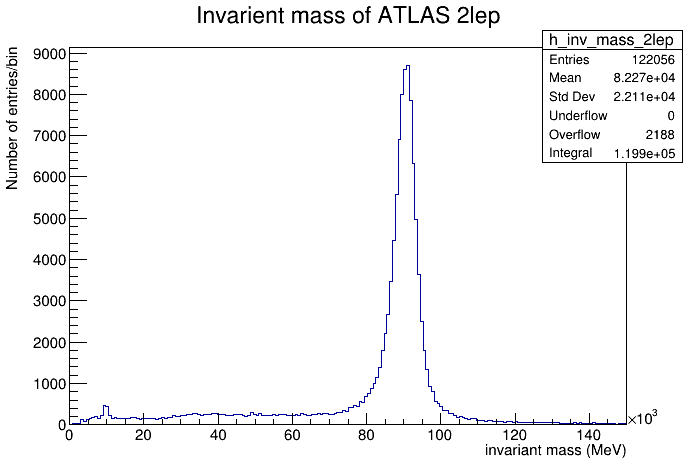
\includegraphics[width=0.85\linewidth]{plots/11-02-2021/2lep-fast_no-cuts_inv-mass_0-150GeV_11-02-21.png}
	\caption{(Exercise 6.4) (Fast) Plot of $Z \rightarrow ll$ invariant mass using MC data. From MC: Mean = (9.018±0.766)e+4 MeV. Expected: (9.1187±0.00021)e+4 MeV.  Cuts: just 2 leptons}
	\label{fig:zll_inv-mass_50-150GeV_11-02-21_11:12}
\end{figure}

\subsubsection*{\textbf{13:00}}
Break for lunch

\subsubsection*{\textbf{14:00} - Lead DG}
Working on exercise 6.7:\\
Plot graphs of ptcone30 and etcone20 for leptons that are same flavour, oppositely charged. (Zee, Zmumu, 2lep)

ptcone30 = scalar sum of track $p_T$ in a cone of R=0.3\\

Create new function 'Ptcones' in "Analysis.py" to plot the Ptcone30 of a specific lepton.

\subsubsection*{\textbf{15:10}}
To start plot ptcone30[0]:
\\
First plot - figure.\ref{fig:ptcone30_Zee_0-4GeV} of large range (0-4 GeV).\\
Data point at 0 GeV then a gap in data to 1 GeV due to. an artifact of the data of 0 - 1 GeV not being detected. \\
Would have expected an exponential decay.

\begin{figure}[h!]
    \centering
	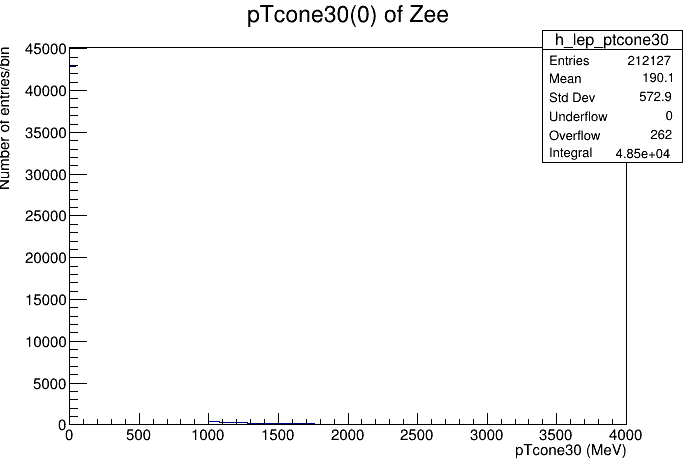
\includegraphics[width=\linewidth]{plots/11-02-2021/Zee-fast_pTcone30(0)_ 0-4Gev_11-02-2021.png}
	\caption{Plot of $Z \rightarrow ll$ pTcone30(0) using MC data. 
	}\label{fig:ptcone30_Zee_0-4GeV}
\end{figure}


\subsubsection*{\textbf{16:00} - Lead BG}

\subsubsection*{\textbf{16:11}}
Question:\\
Why is there not lep\_type = tau??
Plotting the \textbf{invariant mass} of ATLAS experimental data for at least 2 leptons with cuts to select for individual decay paths over energy range 0-150 GeV
\begin{itemize}
    \item $Z \rightarrow ee$ (lep\_type = 11 \&\& 2 particles opposite charge)
    \item $Z \rightarrow \mu\mu$ (lep\_type = 13 \&\& 2 particles opposite charge)
    \item $Z \rightarrow \tau\tau$ (Non ee and non $\tau\tau$)
\end{itemize}

Running e-e pair which is oppositely charged. Figure.\ref{fig:2lep_ee-pair_0-140GeV_11-02-21_16-12} 

\begin{figure}[h!]
    \centering
	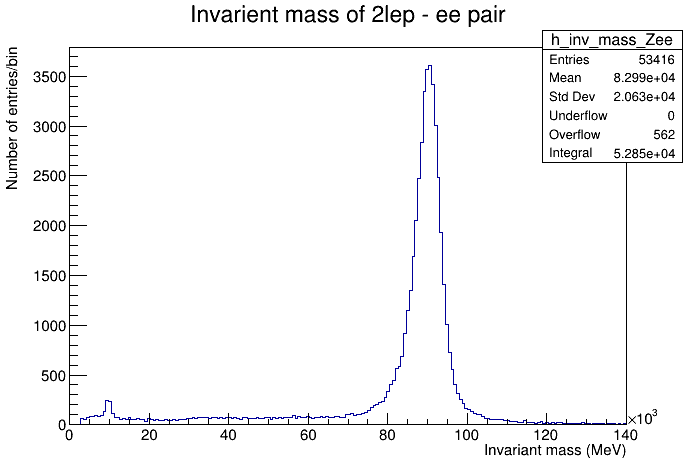
\includegraphics[width=\linewidth]{plots/11-02-2021/2lep-fast_ee-pair_inv-mass_0-140GeV_11-02-21_16-12.png}
	\caption{Plot of $Z \rightarrow ll$ pTcone30 using MC data. 
	}\label{fig:2lep_ee-pair_0-140GeV_11-02-21_16-12}
\end{figure}

Running mu-mu pair which is oppositely charged

Running non e-e and non mu-mu pair which is oppositely charged 
 returned plot no tau-tau pairs with opposite charge 
 
 
%%%%%%%%%%%%%% 16/02/2020 %%%%%%%%%%%%%%%% 
\newpage
%! Author = ben
%! Date = 16/02/2021


%%%%%%%%%%%%%% 16/02/2020 %%%%%%%%%%%%%%%%
\subsection*{\textbf{16/02/2020}}
%%%%%%%%%%%%% 9:00 %%%%%%%%%%%%%
\subsubsection*{\textbf{09:00}}
Discussion of plan for the day:
\begin{itemize}
    \item Finish plotting $Z \rightarrow ll$ plots
    \item Apply cuts to pTCone30 plots
    \item etCone20 plots
\end{itemize}

%%%%%%%%%%%%% 09:23 %%%%%%%%%%%%%
\subsubsection*{09:23 - Lead DG}
Plot etcone20 to investigate what data is available.
\\
Figure.\ref{fig:Zee-fast_ETcone20(0)_0-15GeV_16-02-21_09-34}


plots Fig.\ref{fig:Zee-fast_ETcone20(1)_0-15GeV_16-02-21_09-41} of the etcone20(1)

\\
Both fig.\ref{fig:Zee-fast_ETcone20(0)_0-15GeV_16-02-21_09-34} and fig.\ref{fig:Zee-fast_ETcone20(1)_0-15GeV_16-02-21_09-41} are similar with a larger mean value for fig.\ref{fig:Zee-fast_ETcone20(1)_0-15GeV_16-02-21_09-41}.
\\
Noticed a "bump" at around 4 GeV.
\\
Plan to plot the log of the data to investigate if decay is related to exponential decay.
\begin{figure}[h!]
    \centering
    \begin{minipage}{0.5\textwidth}
        \centering
        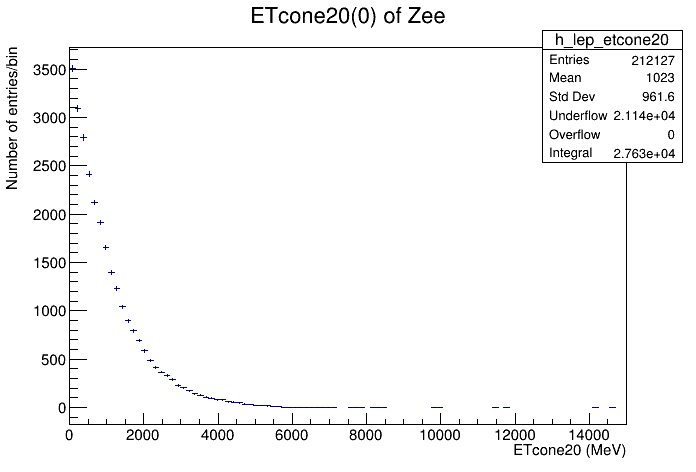
\includegraphics[width=\linewidth]{plots/16-02-2021/Zee-fast_ETcone20(0)_0-15GeV_16-02-21_09-34}
        (A)
    \end{minipage}\hfill
    \begin{minipage}{0.5\textwidth}
        \centering
        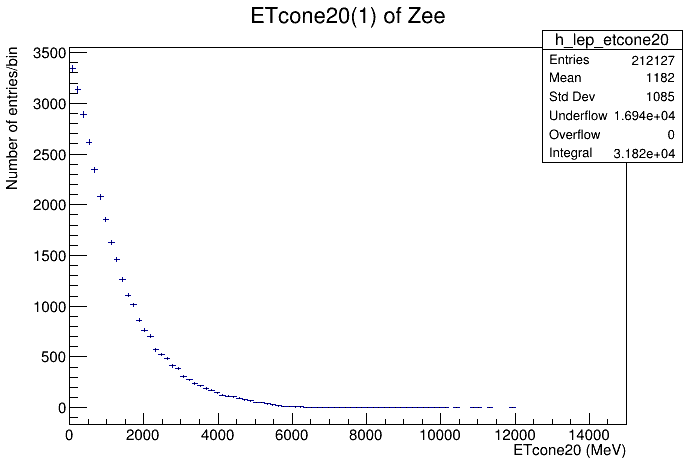
\includegraphics[width=\linewidth]{plots/16-02-2021/Zee-fast_ETcone20(1)_0-15GeV_16-02-21_09-41}
        (B)
    \end{minipage}
    \caption{ (A) Plot of $Z \rightarrow ee$ ETCone20(0) for Zee-fast MC data. (B) Plot of  $Z \rightarrow ee$ ETCone20(1) for Zee-fast MC data.}
    \label{fig:}
\end{figure}

%%%%%%%%%%%%% 09:53 %%%%%%%%%%%%%
\subsubsection*{09:53}
Plotting the ETCone of each of the two leptons produced from the decay of $Z \rightarrow \mu \mu$ using the MC data.
\begin{figure}[h!]
    \centering
    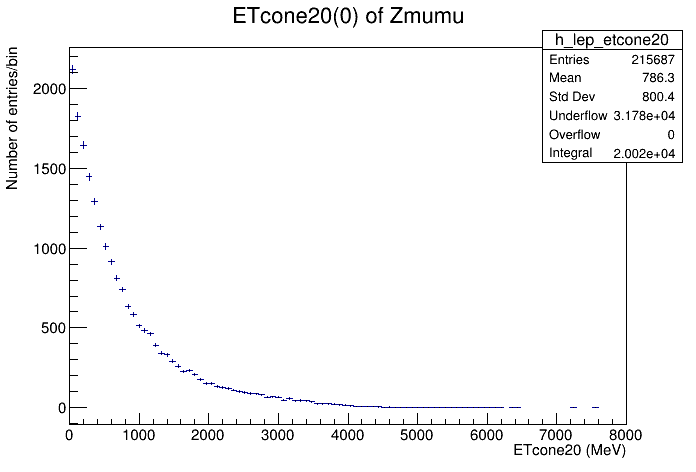
\includegraphics[width=0.85\linewidth]{plots/16-02-2021/Zmumu-fast_ETcone(0)_0-8GeV_16-02-21_09-54.png}
    \caption{Plot of  $Z \rightarrow \mu\mu$ ETCone20(0) for $Z\mu\mu$-fast MC.  data.}\label{fig:Zmumu-fast_ETcone(0)_0-8GeV_16-02-21_09-54}
\end{figure}
On fig\ref{fig:Zmumu-fast_ETcone(0)_0-8GeV_16-02-21_09-54} a slight "bump" at around 1.9 GeV

\begin{figure}[h!]
    \centering
    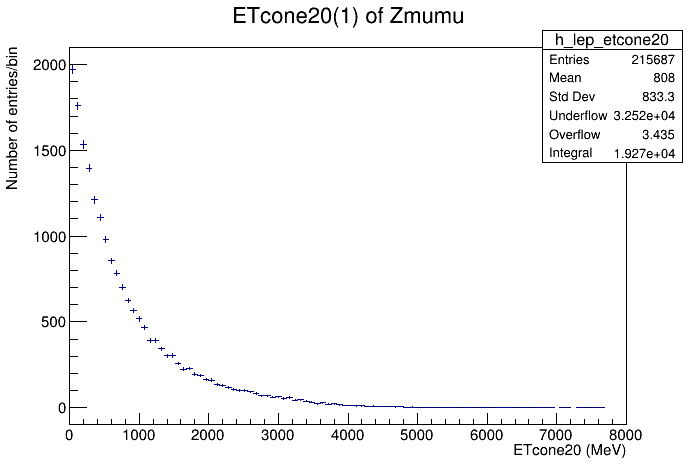
\includegraphics[width=0.85\linewidth]{plots/16-02-2021/Zmumu-fast_ETcone(1)_0-8GeV_16-02-21_09-56.png}
    \caption{Plot of  $Z \rightarrow \mu\mu$ ETCone20(1) for $Z\mu\mu$-fast MC.  data.}\label{fig:Zmumu-fast_ETcone(1)_0-8GeV_16-02-21_09-56}
\end{figure}
On fig.\ref{fig:Zmumu-fast_ETcone(1)_0-8GeV_16-02-21_09-56} the

%%%%%%%%%%%%% 10:07 %%%%%%%%%%%%%
\subsubsection*{10:07}
Plotting the pTCone30 (0)\&(1) of $Z\rightarrow ee$ for the range of 1-4 GeV. This range is used due to 0-1 GeV not being detected. (See 11-02-2021 for the investigation and plots of the full energy range.)

\begin{figure}[h!]
    \centering
    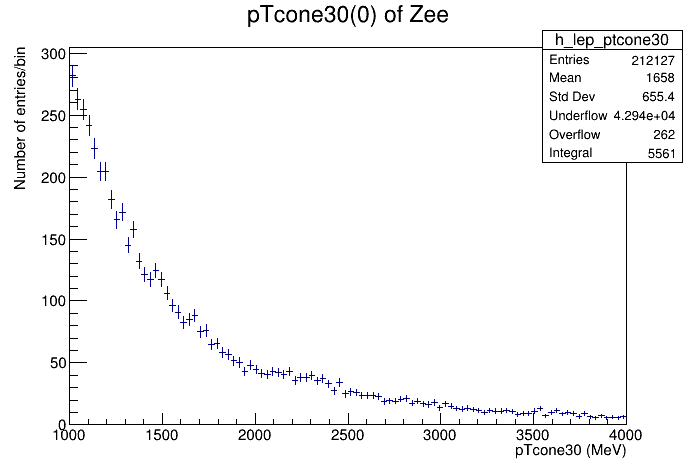
\includegraphics[width=0.85\linewidth]{plots/16-02-2021/Zee_fast_pTcone30(0)_1-4GeV_16-02-21_10-07.png}
    \caption{Plot of  $Z \rightarrow \mu\mu$ pTcone30(0) for $Z\rightarrow ee$-fast MC.  data.}\label{fig:/Zee_fast_pTcone30(0)_1-4GeV_16-02-21_10-07}
\end{figure}

On fig.\ref{fig:/Zee_fast_pTcone30(0)_1-4GeV_16-02-21_10-07}, the number of entries decrease exponentially as momentum increases.  There is also a "bump" around pTcone30 = 2.25GeV

\begin{figure}[h!]
    \centering
    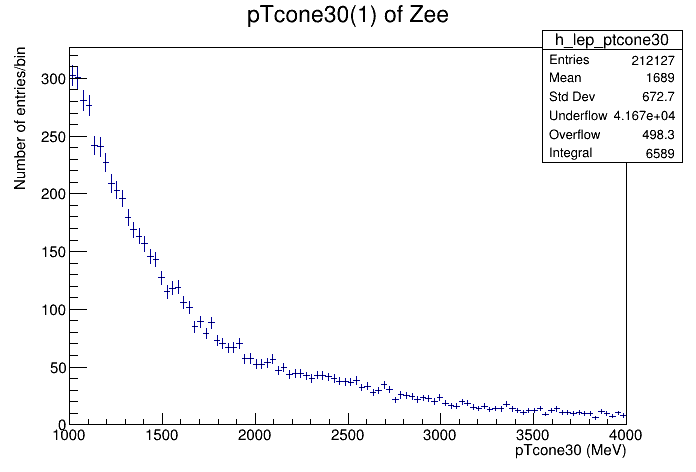
\includegraphics[width=0.85\linewidth]{plots/16-02-2021/Zee_fast_pTcone30(1)_1-4GeV_16-02-21_10-12.png}
    \caption{Plot of  $Z \rightarrow \mu\mu$ pTcone30(1) for $Z\rightarrow ee$-fast MC.  data.}\label{fig:Zee_fast_pTcone30(1)_1-4GeV_16-02-21_10-12}
\end{figure}

In fig.\ref{fig:Zee_fast_pTcone30(1)_1-4GeV_16-02-21_10-12} to "bump" seen is not as pronounced as in fig.\ref{fig:/Zee_fast_pTcone30(0)_1-4GeV_16-02-21_10-07}.


%%%%%%%%%%%%% 10:18 %%%%%%%%%%%%%
\subsubsection*{10:18}
Plotting the pTCone30 (0)\&(1) of $Z\rightarrow \mu\mu$ for the range of 1-4 GeV. This range is used due to 0-1 GeV not being detected. (See 11-02-2021 for the investigation and plots of the full energy range.)

\begin{figure}[h!]
    \centering
    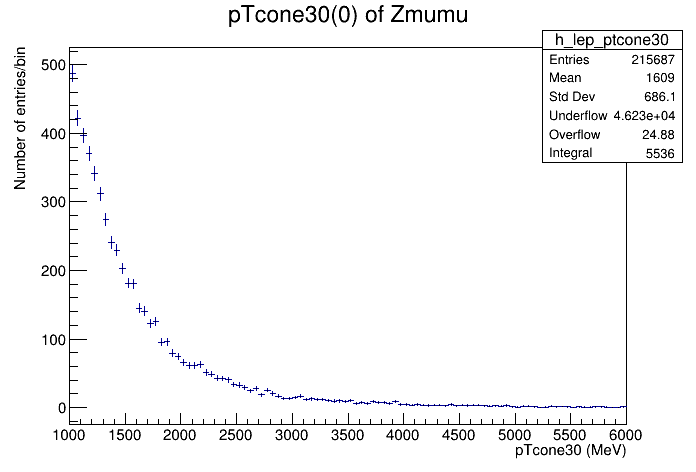
\includegraphics[width=0.85\linewidth]{plots/16-02-2021/Zmumu_fast_pTcone30(0)_1-6GeV_16-02-21_10-18.png}
    \caption{Plot of  $Z \rightarrow \mu\mu$ pTcone30(0) for $Z\mu\mu$-fast MC.  data.}\label{fig:Zmumu_fast_pTcone30(0)_1-6GeV_16-02-21_10-18}
\end{figure}

\begin{figure}[h!]
    \centering
    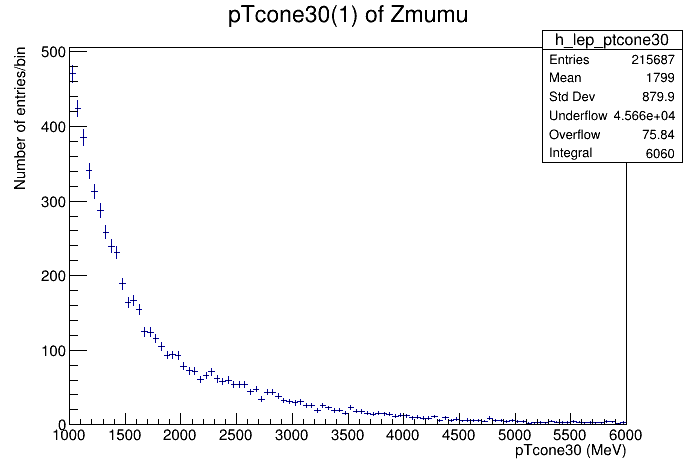
\includegraphics[width=0.85\linewidth]{plots/16-02-2021/Zmumu_fast_pTcone30(1)_1-6GeV_16-02-21_10-21.png}
    \caption{Plot of  $Z \rightarrow \mu\mu$ pTcone30(1) for $Z\mu\mu$-fast MC.  data.}\label{fig:Zmumu_fast_pTcone30(1)_1-6GeV_16-02-21_10-21}
\end{figure}


%%%%%%%%%%%%% 10:40 %%%%%%%%%%%%%
\subsubsection*{10:40}
Plotting the pTcone30 (total (sum of the two leptons)) of ATLAS data with cuts:
\begin{itemize}
    \item opposite charge
    \item lep\_type == 11 (lepton type = electron)
    \item lep\_n == 2 (number of leptons = 2)
\end{itemize}
To start, plot the range of 0-10 GeV to show 0-1 GeV is not detected.  This is seen in Fig.\ref{fig:2lep_fast_ee-pair_pTcone30(total)_0-10GeV_16-02-21_10-50} with a peak value at (total) pTcone30
\begin{figure}[h!]
    \centering
    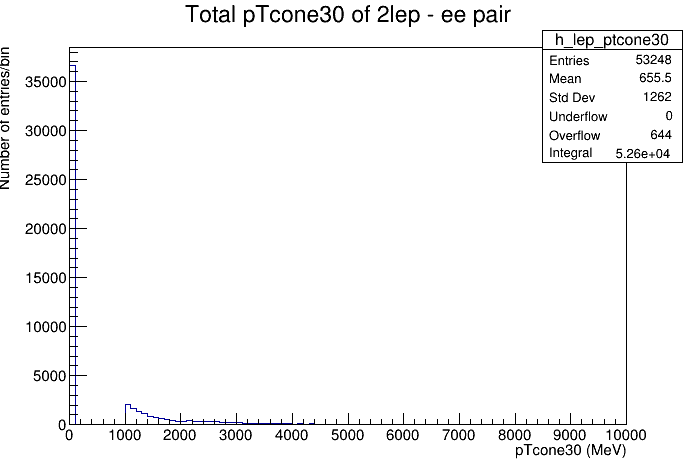
\includegraphics[width=0.85\linewidth]{plots/16-02-2021/2lep_fast_ee-pair_pTcone30(total)_0-10GeV_16-02-21_10-50}
    \caption{Plot of  $Z \rightarrow \mu\mu$ pTcone30(1) for $Z\mu\mu$-fast MC.  data.}\label{fig:2lep_fast_ee-pair_pTcone30(total)_0-10GeV_16-02-21_10-50}
\end{figure}


\begin{figure}[h!]
    \centering
    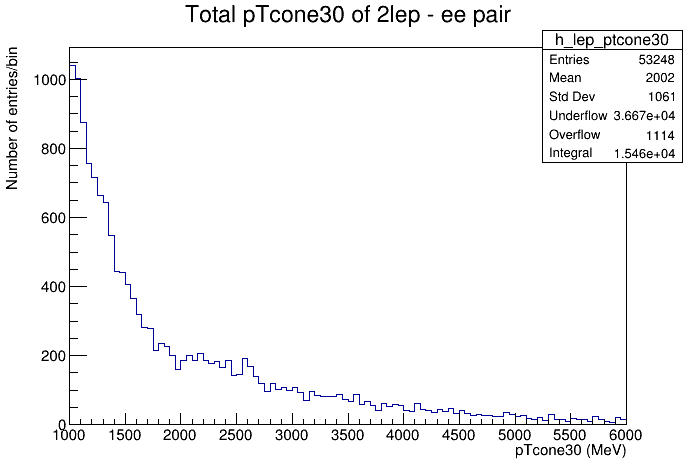
\includegraphics[width=0.85\linewidth]{plots/16-02-2021/2lep_fast_ee-pair_pTcone30(total)_1-6GeV_16-02-21_10-59}
    \caption{Plot of  $Z \rightarrow \mu\mu$ pTcone30(1) for $Z\mu\mu$-fast MC.  data.}\label{fig:2lep_fast_ee-pair_pTcone30(total)_1-6GeV_16-02-21_10-59}
\end{figure}

Fig.\ref{fig:2lep_fast_ee-pair_pTcone30(total)_1-6GeV_16-02-21_10-59} has the range set to 1-6 GeV (to remove the un-detected regoin 0-1 GeV).  This still shows exponential like decay as pTcone increases. \\
The "bump"/inconsistency (if expecting smooth exponential like decay) is present in the experiental ATLAS data around 2-2.7 GeV.  To investigate this bump, plan to plot the invariant mass with a cut to select for a pTcone30 in the vicinity of 2-2.7 GeV.

%%%%%%%%%%%%% 11:10 %%%%%%%%%%%%%
\subsubsection*{11:10}
Plotting ATLAS 2lep data for the total ETCone20 for a ee pair in the range of 0-6 GeV.  This can be seen in Fig.\ref{fig:2lep_fast_ee-pair_ETcone30(total)_0-6GeV_16-02-21_11-11}

\begin{figure}[h!]
    \centering
    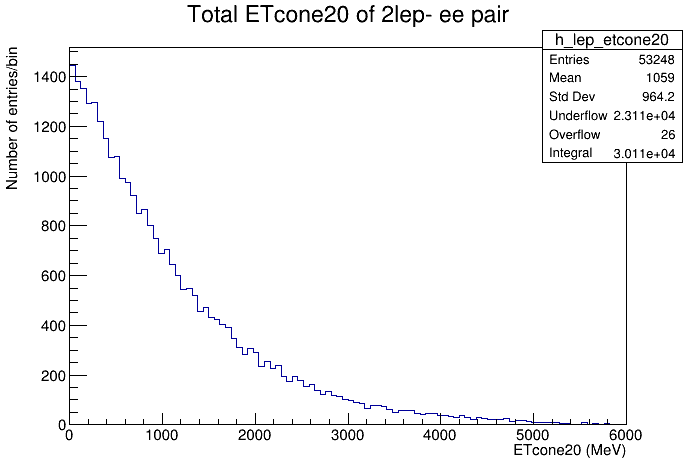
\includegraphics[width=0.85\linewidth]{plots/16-02-2021/2lep_fast_ee-pair_ETcone30(total)_0-6GeV_16-02-21_11-11}
    \caption{Plot of the total ETCone20 of an ee pair using the 2lep-fast ATLAS data.  data.}\label{fig:2lep_fast_ee-pair_ETcone30(total)_0-6GeV_16-02-21_11-11}
\end{figure}

%%%%%%%%%%%%% 11:14 %%%%%%%%%%%%%
\subsubsection*{11:14}

\begin{figure}[h!]
    \centering
    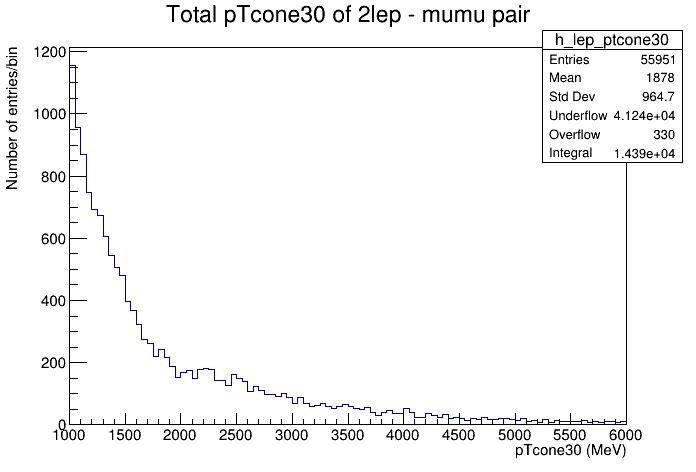
\includegraphics[width=0.85\linewidth]{plots/16-02-2021/2lep_fast_mumu-pair_pTcone30(total)_1-6GeV_16-02-21_11-06}
    \caption{Plot of the total pTcone30 of a mumu pair using the 2lep-fast ATLAS data. }\label{fig:2lep_fast_mumu-pair_pTcone30(total)_1-6GeV_16-02-21_11-06}
\end{figure}

\begin{figure}[h!]
    \centering
    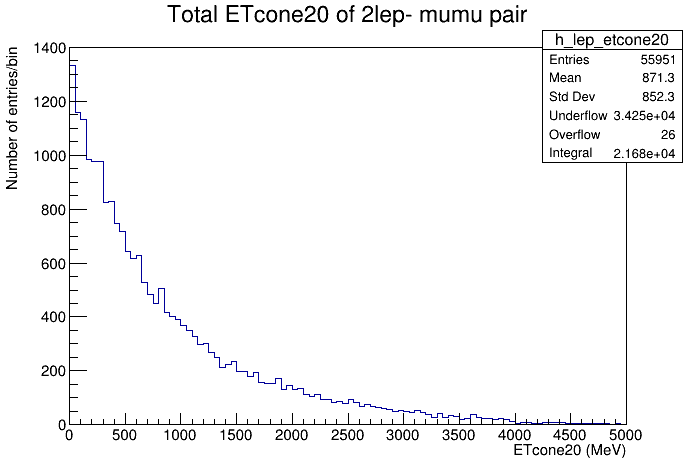
\includegraphics[width=0.85\linewidth]{plots/16-02-2021/2lep_fast_mumu-pair_ETcone30(total)_0-5GeV_16-02-21_11-14}
    \caption{Plot of the total ETcone20 of a mumu pair using the 2lep-fast ATLAS data. }\label{fig:2lep_fast_mumu-pair_ETcone30(total)_0-5GeV_16-02-21_11-14}
\end{figure}



%%%%%%%%%%%%% 11:24 %%%%%%%%%%%%%
\subsubsection*{11:24 - Lead BG}
To investigate the possible bump or dip (as seen in the pTcone30 data (bump around \dots  or dip around \dots)) plot the log of the ptCone30.


%2lep mumu logs


%pTcone
\begin{figure}[h!]
    \centering
    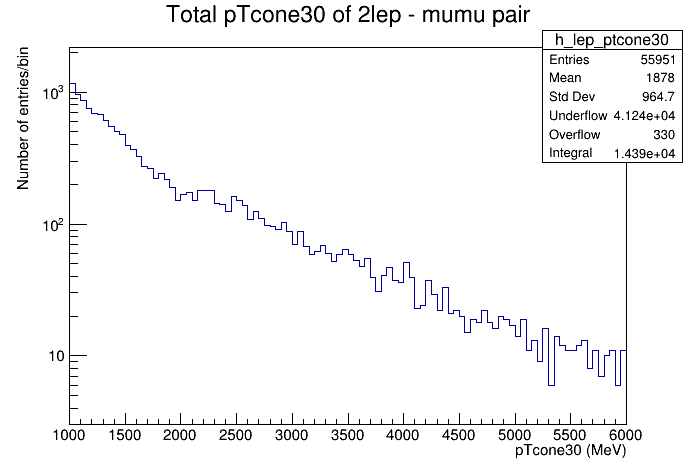
\includegraphics[width=0.85\linewidth]{plots/16-02-2021/2lep-fast_mumu_ptcone30(total)_log-entries_1-6GeV_16-02-2021_11-39}
    \caption{Plot of the total pTcone30 of a mumu pair using the 2lep-fast ATLAS data, log. }\label{fig:2lep-fast_mumu_ptcone30(total)_log-entries_1-6GeV_16-02-2021_11-39}
\end{figure}




\begin{figure}[h!]
    \centering
    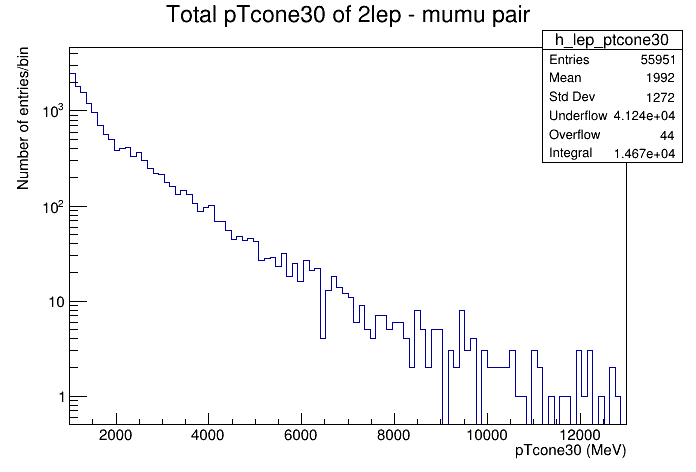
\includegraphics[width=0.85\linewidth]{plots/16-02-2021/2lep-fast_mumu-pair_ptcone30(total)_log-entries_1-13GeV_16-02-2021_11-45}
    \caption{Plot of the total pTcone30 of a mumu pair using the 2lep-fast ATLAS data, log,1-13GeV. }\label{fig:2lep-fast_mumu-pair_ptcone30(total)_log-entries_1-13GeV_16-02-2021_11-45}
\end{figure}

\begin{figure}[h!]
    \centering
    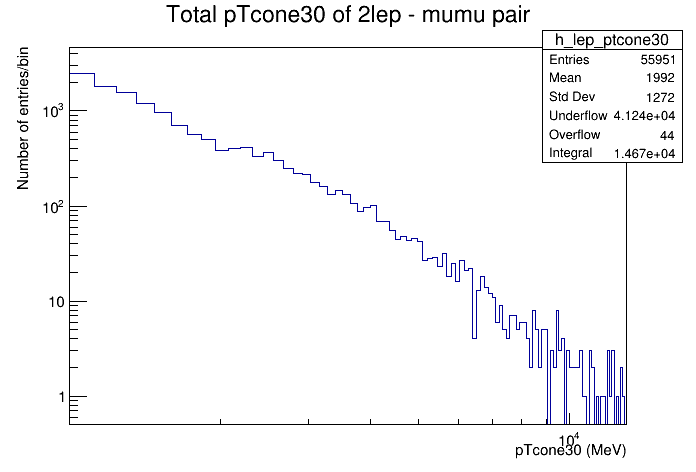
\includegraphics[width=0.85\linewidth]{plots/16-02-2021/2lep-fast_mumu-pair_ptcone30(total)_log-log_1-13GeV_16-02-2021_11-45}
    \caption{Plot of the total pTcone30 of a mumu pair using the 2lep-fast ATLAS data, log-log,1-13GeV. }\label{fig:2lep-fast_mumu-pair_ptcone30(total)_log-log_1-13GeV_16-02-2021_11-45.png}
\end{figure}


%ETcone
\begin{figure}[h!]
    \centering
    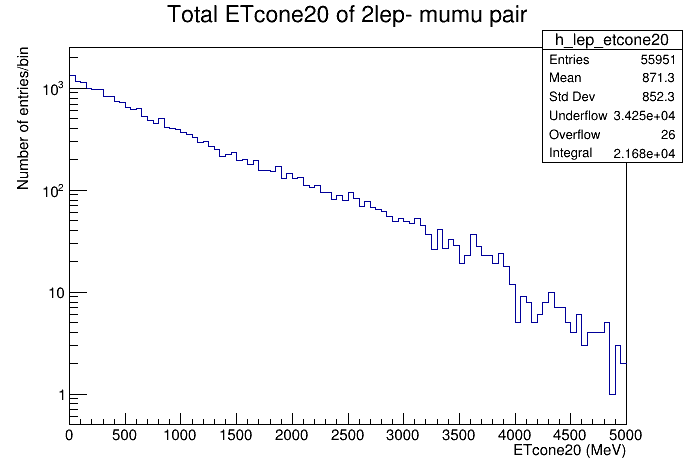
\includegraphics[width=0.85\linewidth]{plots/16-02-2021/2lep-fast_mumu-pair_etcone20(total)_log-entries_0-5GeV_16-02-2021_11-31}
    \caption{Plot of the total ETcone20 of a mumu pair using the 2lep-fast ATLAS data, log, 0-5GeV. }\label{fig:2lep-fast_mumu-pair_etcone20(total)_log-entries_0-5GeV_16-02-2021_11-31}
\end{figure}

\begin{figure}[h!]
    \centering
    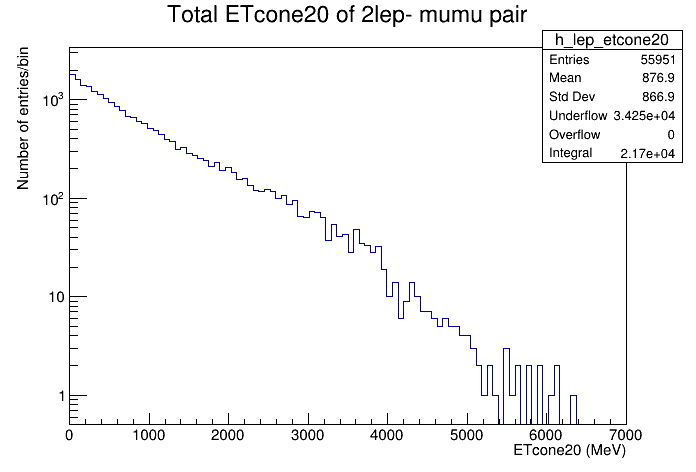
\includegraphics[width=0.85\linewidth]{plots/16-02-2021/2lep-fast_mumu-pair_etcone20(total)_log-entries_0-7GeV_16-02-2021_11-33.png}
    \caption{Plot of the total ETcone20 of a mumu pair using the 2lep-fast ATLAS data, log,0-7GeV. }\label{fig:2lep-fast_mumu-pair_etcone20(total)_log-entries_0-7GeV_16-02-2021_11-33}
\end{figure}

\subsection*{14:06- BG lead}\\
Investigate use of stacked MC plots to identify background when comparing to ATLAS data.//

\subsection*{14:50}\\
Stacked plot made for invariant. mass

\subsubsection*{16:20}
Stacked plot made for mean etcone20, includes
\begin{itemize}
    \item 2lep data
    \item Zee MC
    \item Zmumu MC
    \item Ztautau MC
\end{itemize}

\begin{figure}[h!]
    \centering
    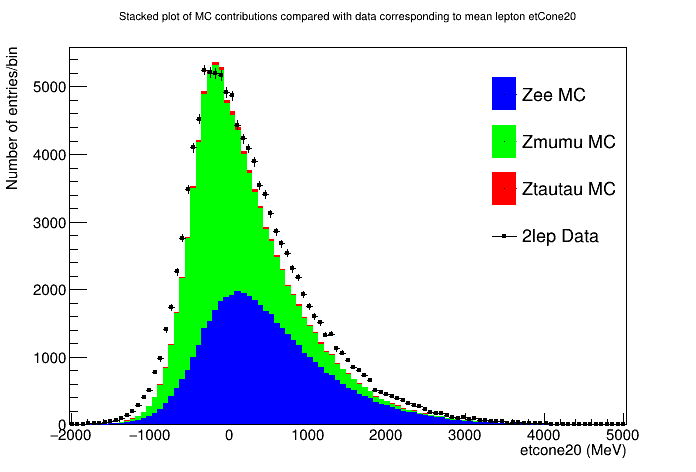
\includegraphics[width=0.85\linewidth]{plots/16-02-2021/2lep-Zee-Zmumu-Ztautau-fast_mean-etcone20_-2-5GeV_16-02-21_16-28}
    \caption{Stack plot of the mean ETcone20 of 2 lep with opposite charge pair using the 2lep-fast ATLAS data, log,0-7GeV. }\label{fig:2lep-Zee-Zmumu-Ztautau-fast_mean-etcone20_-2-5GeV_16-02-21_16-28}
\end{figure}


\subsubsection*{16:28}
Unexplained discrepancy of 2lep data around peak ~$0$MeV (Fig.\ref{fig:2lep-Zee-Zmumu-Ztautau-fast_mean-etcone20_-2-5GeV_16-02-21_16-28})

%%%%%%%%%%%%%% 18/02/2020 %%%%%%%%%%%%%%%% 
\newpage
%%%%%%%%%%%%%% 18/02/2020 %%%%%%%%%%%%%%%% 
\subsection*{\textbf{18/02/2020}}
\subsubsection*{Days Aim}
\begin{itemize}
    \item Start to look at cross section
\end{itemize}

\subsubsection*{Day Summary}
\begin{itemize}
    \item Investigated background contributions from $ttbar_lep$, $Wplus_2lep$, and $Wminus_2lep$
    \item Calculated a preliminary value for $\sigma (Z \rightarrow ee)$ to be
    \subitem $\sigma (Z \rightarrow ee) = 1.943 nb$
\end{itemize}
%%%%%%%%%%%%% 9:00 %%%%%%%%%%%%%
\subsubsection*{09:00 - Lead BG}
Integrated Luminosity = $139 \text{fb}^{-1} (\pm 1.7\%)$

Coeficient $\epsilon$ given by sum of MC signal weights over that for relevent sample (found using TotExpected.Py) 

Made stacked plots for pTcone30 and etcone. Unexplained discrepancy of 2lep data aorund peak ~$0$MeV (Figure \ref{fig:2lep-Zee-Zmumu-Ztautau-fast_mean-etcone20_-2-5GeV_16-02-21_16-28}) 


Add ttbar\_lep to stack plots


$\epsilon_{\text{Zee}}$ = 19630128.89 

Quoted value for Zee cross section $76.0 \pm 0.8 \pm 2.0 \pm 2.6$ pb (https://arxiv.org/pdf/1212.4620.pdf)

%%%%%%%%%%%%% 10:38 %%%%%%%%%%%%%
\subsubsection*{10:38}

Rough estimate for the cross section: $\sigma (pp \rightarrow Z \rightarrow ee)$ is given by:
\begin{align}
    \sigma &= \frac{N^{selected} - N^{background}}{\epsilon \int L dt}
\end{align}
where
\begin{align}
     \epsilon &= \frac{\sum \text{weights for all MC events which pass selection cuts}}{\sum \text{weights for all events for that process}} 
\end{align}
For $Z \rightarrow ee$ use the cuts:
\begin{itemize}
    \item lep\_n = 2
    \item same flavour/type (lep\_type [0] == lep\_type[1])
    \item opposite charge (lep\_charge [0] != lep\_charge[1])
    \item invariant mass > 60 GeV 
    \subitem MC not modelled below this point
\end{itemize}
For $\sigma (pp \rightarrow Z \rightarrow ee)$:
\begin{itemize}
    \item $N^{selected} = 47531$
    \item $N^{background} = 0$
    \item $\epsilon = \frac{46740}{19630128.89} = $
    \item $\int L dt = 10.064 \textbf{fb}^{-1}$
\end{itemize}


cs = 1.9835391029941325e-09
\\
Other sources of background 
 - photon conversion 
 - hadronic jets
 -W or t decays can be detected as 2 electrons or muons when one is in fact a hadron jet or electron/moun from other source. 
 
%%%%%%%%%%%%% 14:00 %%%%%%%%%%%%%
\subsubsection*{14:00 - Lead DG - Number of leptons from W-plus and W-minus}
Investigating the decay paths of W-plus and W-minus.
\\
Plotting the number of leptons per event ($lep_n$)
\\
Cuts used in Fig.\ref{fig:14-00_18-02-21}:
\begin{lstlisting}
lepCut = "(" + "(lep_charge[0] != lep_charge[1]) && (lep_type[0] == lep_type[1]) && lep_n==2" + ")"

t.Draw("lep_n >> h_lep_n(100,0,100)", weighting + "*" + lepCut)
\end{lstlisting}
\begin{figure}[h!]
    \centering
    \begin{minipage}{0.5\textwidth}
        \centering
        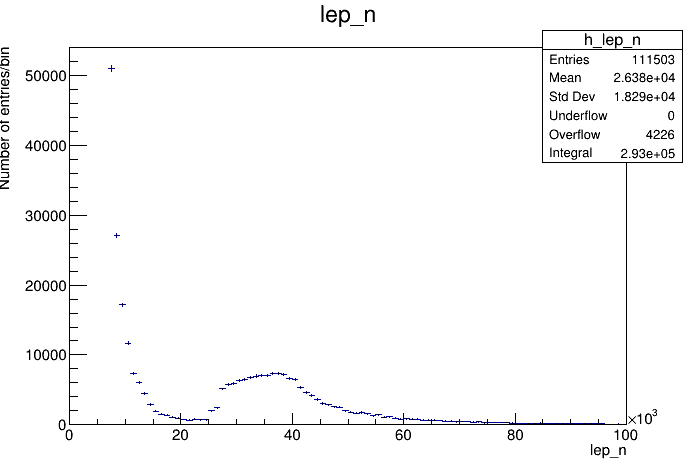
\includegraphics[width=\linewidth]{plots/18-02-2021/Wminus_2lep_lep_n_0-100_18-02-2021_14-12.png}
        (A)
    \end{minipage}\hfill
    \begin{minipage}{0.5\textwidth}
        \centering
        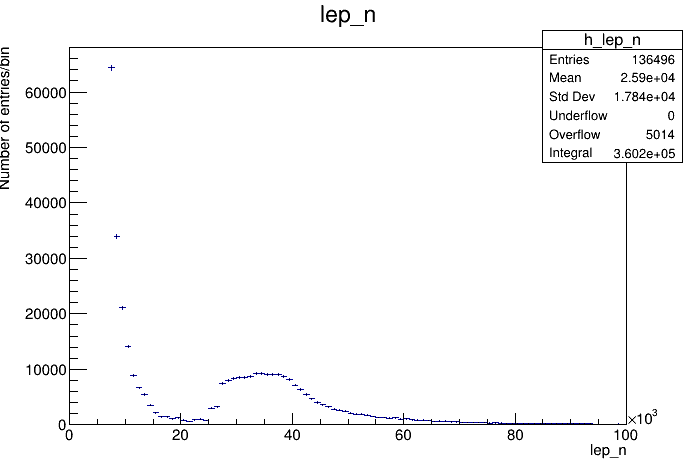
\includegraphics[width=\linewidth]{plots/18-02-2021/Wplus_2lep_slow_lep_n_0-100000_18-02-21_14-17.png}
        (B)
    \end{minipage}
    \caption{(A) Number of leptons in each event for Wminus-2lep. (B) Number of leptons in each event for Wplus-2lep. Cuts = basic: lepton pair with opposite charge and same type.}
    \label{fig:14-00_18-02-21}
\end{figure}
% (A) Wminus_2lep_lep_n_0-100_18-02-2021_14-12.png
% (B) Wplus_2lep_slow_lep_n_0-100000_18-02-21_14-17.png

There is an exponential decay in the number of leptons apart from a bump at about 35 leptons.
\\
This indicates that these leptons are most likely a result of lepton showers/jets.


%%%%%%%%%%%%% 14:40 %%%%%%%%%%%%%
\subsubsection*{14:40 - Invariant mass for Wplus-2lep and Wminus-2lep (Z -> ll)}
Plot the invariant mass between 60-150GeV for Wplus-2lep and Wminus-2lep for events that would look like $Z \rightarrow ll$.
\\
Large underflow, so increase range to 0-150 GeV 
\\
Still not totally decayed, increase range to 0-500 GeV.
\\
Cuts used in. Fig.\ref{fig:14-40_18-02-2021}:
\begin{lstlisting}
lepCut = "(" + "lep_n == 2 && (lep_charge[0] != lep_charge[1]) &&  (lep_type[0] == lep_type[1]) " + ")"

t.SetAlias("inv_mass_Zll","sqrt(2*lep_pt[0]*lep_pt[1]*(cosh(lep_eta[0]-lep_eta[1])-cos(lep_phi[0]-lep_phi[1])))")
  
t.Draw("inv_mass_Zll >> h_inv_mass(100,0,150e3)", weighting + "*" + lepCut)
\end{lstlisting}
\begin{figure}[h!]
    \centering
    \begin{minipage}{0.5\textwidth}
        \centering
        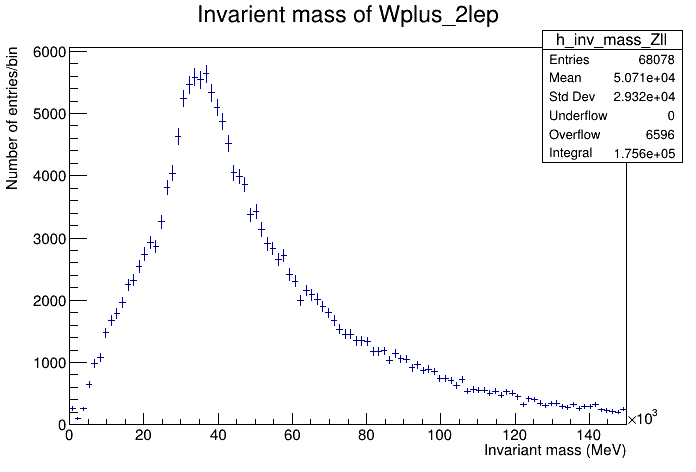
\includegraphics[width=\linewidth]{plots/18-02-2021/Invarient mass of Wplus_2lep 18-02-2021_14_49 .png}
        (A)
    \end{minipage}\hfill
    \begin{minipage}{0.5\textwidth}
        \centering
        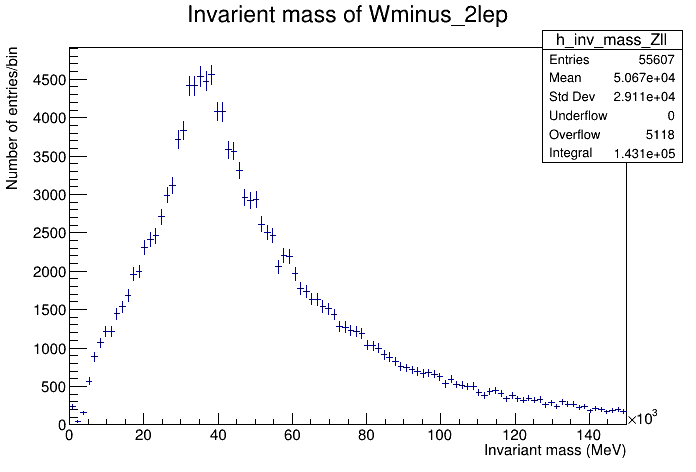
\includegraphics[width=\linewidth]{plots/18-02-2021/Wminus-2lep_invar-mass_18-02-21_14-54.png}
        (B)
    \end{minipage}
    \caption{(A) Invariant mass from Wplus-2lep (Background contribution) (B) Invariant mass from Wminus-2lep.  Cuts: (basic) lepton pair with oppsite charge and same type.}
    \label{fig:14-40_18-02-2021}
\end{figure}


%%%%%%%%%%%%% 16:10 %%%%%%%%%%%%%
\subsubsection*{16:00 - Lead BG - preliminary $\sigma (Z \rightarrow ee)$}
Finding the background contributions from $W^+ \rightarrow l\nu_l $ with the cut 
\begin{lstlisting}
     lepCut ="(" + "(lep_charge[0] != lep_charge[1]) && (lep_type[0]==11 && lep_type[1]==11) && lep_n==2 && (inv_mass_Zll > 60e3) && (inv_mass_Zll < 115e3)" + ")"
\end{lstlisting}
to select for e+e- pair.
\begin{align}
    N^{background}_{t\Bar{t}} &= 236276
    \\
    N^{background}_{W^+} &= 2247
    \\
    N^{background}_{W-} &= 1785
\end{align}
Sum of all weights for all MC events which pass cuts for Zee:
\begin{align*}
    = 4595000
\end{align*}
 
4817004

$\sigma(Z \rightarrow ee) = 1.94275964340403e-09 b$

//
TODO: 
\begin{itemize}
    \item Plot $ \Delta \phi$ 
    \item $\epsilon$ cut
\end{itemize}





%%%%%%%%%%%%%% 23/02/2020 %%%%%%%%%%%%%%%% 
\newpage
%%%%%%%%%%%%%% 23/02/2020 %%%%%%%%%%%%%%%% 
\subsection*{\textbf{23/02/2020}}

\subsubsection*{Days aims}
\begin{itemize}
    \item Investigate $\Delta \phi$
    \item 
\end{itemize}

\subsubsection*{Day Summary}
\begin{itemize}
    \item Investigated $\Delta \phi$
    \item Applied ptcone30 cut to invariant mass
    \item Plotted etcone20 with ptcone30 cuts
    
    \item Found pT upper cut of:
    \subitem 34 GeV for mumu 
    \subitem 36 GeV for ee 
    
    \item Plotted $\eta$ - ruled out as a cut
    
    \item 
\end{itemize}
%%%%%%%%%%%%% 9:00 %%%%%%%%%%%%%
\subsubsection*{08:30 - Lead BG}
The ATLAS detector can mistake the production of a $l^+ l^-$ pair from 2 seperate decays as pair production from the decay of a single particle, such as a Z boson. 
\\
A possible source of this is from W boson decays:
\begin{align*}
    W^+ \rightarrow l^+ \nu_{l}
    \\
    W^- \rightarrow l^- \Bar{\nu_{l}}
\end{align*}
to be mistaken for $Z \rightarrow ll$.
\\
In the case of $Z \rightarrow ll$, the two leptons would be expected to be produced with the angle between them ($\Delta \phi$) $\approx \pi$ (angle between the azimuthal angle) to conserve momentum.
\\
Counter to this, the  $W^+ \rightarrow l^+ \nu_{l}$ and $W^- \rightarrow l^- \Bar{\nu_{l}}$ can be proceed at any angle, so would expect production to include $\Delta \phi \approx 0$
\\
To investigate this, plot $\Delta \phi$ of ATLAS "2lep" data, the cuts used in Fig.\ref{fig:23-02_09-43} are:
\begin{lstlisting}
lepCut ="(" + "(lep_charge[0] != lep_charge[1]) && (lep_type[0]==13 && lep_type[1]==13) && lep_n==2 && (inv_mass_Zll > 60e3)" + ")"
    
t.SetAlias("inv_mass_Zll","sqrt(2*lep_pt[0]*lep_pt[1]*(cosh(lep_eta[0]-lep_eta[1])-cos(lep_phi[0]-lep_phi[1])))")

t.Draw("abs(lep_phi[0] - lep_phi[1]) >> h_lep_delta_phi(100,0,6.3)", weighting + "*" + lepCut)
\end{lstlisting}

Fig.\ref{fig:23-02_09-43} shows that there is a small peak at loer angles.  This can be produced from. two main processes:
\begin{itemize}
    \item Momentum conservation to compensate for jets
    \item incorrect classification for two W+ and W- decays.
\end{itemize}

\begin{figure}[h!]
    \centering
    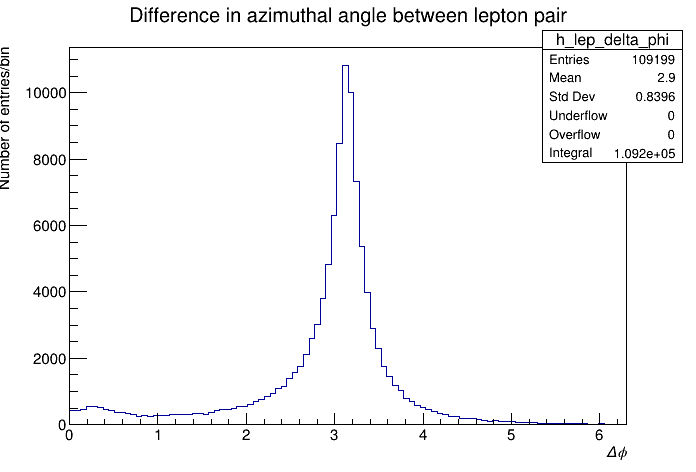
\includegraphics[width=0.85\linewidth]{plots/23-02-2021/2lep_delta-phi_0-7_23-02_09-43.png}
    \caption{The difference of the azimuthal angle of the lepton pair for the 2lep ATLAS data.  The main peak at approx $\pi$ is as expected}\label{fig:23-02_09-43}
\end{figure}

%%%%%%%%%%%%% 9:48 %%%%%%%%%%%%%
\subsubsection*{09:48 - Lead DG}
Apply ptcone20 cut on invariant mass plots.
\\
Since there is no distinction between events in the range 0-1 GeV, cut events above 1 GeV.
\\
Since variables/quantities are correlated (can be effected by the same physical process), plot the etcone20 stack plot.   See Fig.\ref{}

%%%%%%%%%%%%% 14:07 %%%%%%%%%%%%%
\subsubsection*{14:07 - Lead BG}
Plot pT log to test for potential cuts.

Test other kinematic variables to look for potential cuts

Upper bound cut of 320GeV for total lepton pair pT.  See Fig.{}

%%%%%%%%%%%%% 15:24 %%%%%%%%%%%%%
\subsubsection*{15:24 - Lead DG - Plot $\eta$}
Plot eta in search of potential cuts. 
\\
Cuts used for Fig.\ref{fig:15-24_23-02-21}:
\begin{lstlisting}
lepCut ="(" + "(lep_charge[0] != lep_charge[1]) && (lep_type[0]==lep_type[1]) && lep_n==2" + ")"
    
t.Draw("abs(lep_eta[0]) >> h_lep_eta(100,0,3)", weighting + "*" + lepCut)
\end{lstlisting}
\begin{figure}[h!]
    \centering
	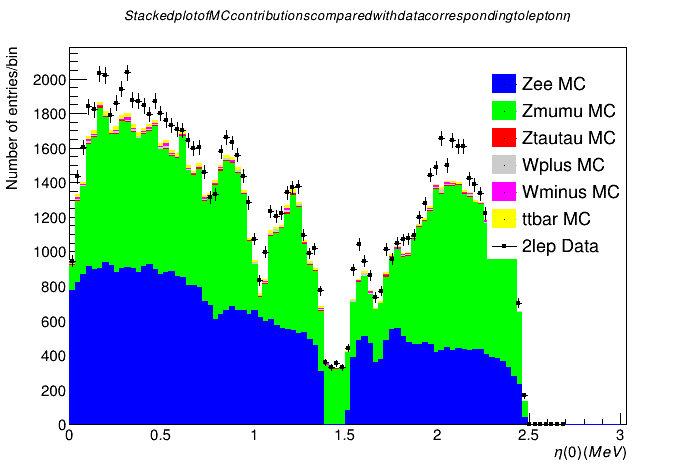
\includegraphics[width=0.85\linewidth]{plots/23-02-2021/All-stack-fast_eta_0-3_.png}
	\caption{Stack plot for the absolute value of $eta$ for lepton [0] to include signal and and background 2lep and MC.  Cuts: lepton pair of same flavour/type and opposite charge. }\label{fig:15-24_23-02-21}
\end{figure}


%%%%%%%%%%%%% 15:31 %%%%%%%%%%%%%
\subsubsection*{15:31}
Plot the stack plot of delta phi in search of possible cuts.
\\
First apply only minimal cuts (no lower from invariant mass and upper ):
\begin{lstlisting}
lepCut ="(" + "(lep_charge[0] != lep_charge[1]) && (lep_type[0]==13 && lep_type[1]==13) && lep_n==2 && (inv_mass_Zll > 60e3)" + ")"
    
t.SetAlias("inv_mass_Zll","sqrt(2*lep_pt[0]*lep_pt[1]*(cosh(lep_eta[0]-lep_eta[1])-cos(lep_phi[0]-lep_phi[1])))")

t.Draw("abs(lep_phi[0] - lep_phi[1]) >> h_lep_delta_phi(100,0,6.3)", weighting + "*" + lepCut)
\end{lstlisting}
\begin{figure}[h!]
    \centering
	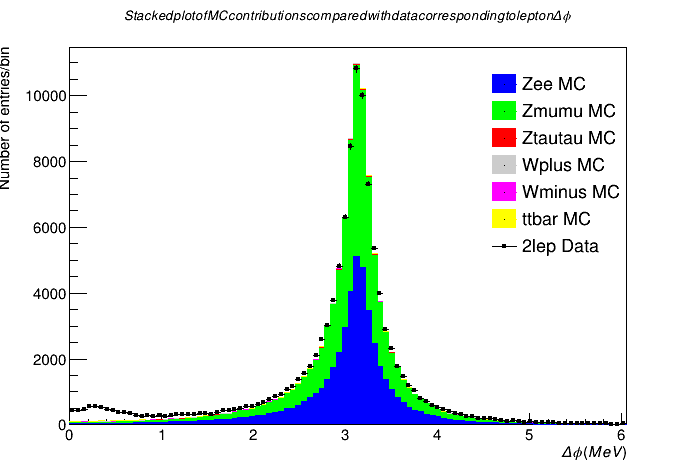
\includegraphics[width=0.85\linewidth]{plots/23-02-2021/All-stack-fast_delta-phi_minimal-cuts_0-6_23-02-21_15-30.png}
	\caption{Stack plot of delta phi with only minimal cuts to select for events with 2 leptons of same type with opposite charge.  There is an inconstancy between MC and ATLAS data (\textbf{NOT MeV - should be rad})}\label{fig:All-stack-fast_delta-phi_minimal-cuts_0-6_23-02-21_15-30}
\end{figure}
From Fig.\ref{fig:All-stack-fast_delta-phi_minimal-cuts_0-6_23-02-21_15-30}:
- Inconstancy between MC and ATLAS data around 0-1 rad.

Now add upper from total transverse momentum and lower from invariant mass.
\begin{figure}[h!]
    \centering
	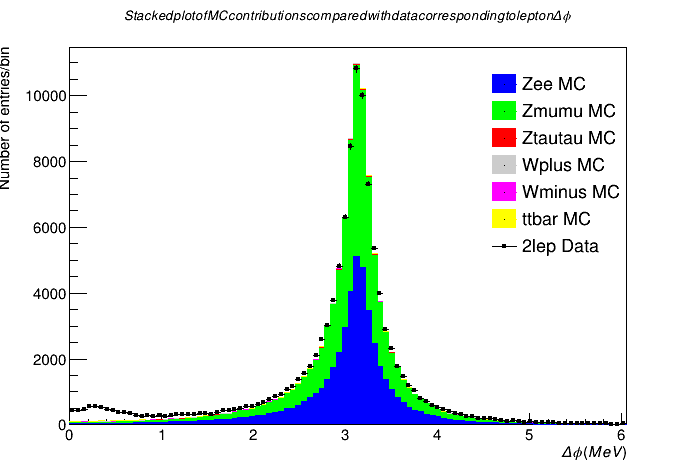
\includegraphics[width=0.85\linewidth]{plots/23-02-2021/All-stack-fast_delta-phi_minimal-cuts_0-6_23-02-21_15-30.png}
	\caption{Stack plot of delta phi with only minimal cuts to select for events with 2 leptons of same type with opposite charge.  There is an inconsitancy between MC and ATLAS for $\Delta \phi < 1 rad$ (\textbf{NOT MeV - should be rad})}\label{fig:All-stack-fast_delta-phi_minimal-cuts_0-6_23-02-21_15-30}
\end{figure}
From Fig.\ref{}:
-> Good MC fit to ATLAS data - no more "bump" between 0-1 rad

Question: Is it better to make cuts based on individual particles or total/mean.
 
 %%%%%%%%%%%%% 15:54 %%%%%%%%%%%%%
\subsubsection*{15:54 - Lead BG}
Start to calculate the cross section of $pp \rightarrow Z \rightarrow ee$ with the new cuts (lower and upper bounds on variables).
\\
Cuts being used:
\begin{lstlisting}
lepCut ="(" + "(lep_charge[0] != lep_charge[1]) && (lep_type[0]==lep_type[1]) && lep_n==2 && (inv_mass_Zll > 60e3) && (lep_pt[0]+lep_pt[1]) < 320e3 " + ")"
\end{lstlisting}

%%%%%%%%%%%%% 17:00 %%%%%%%%%%%%%
\subsubsection*{17:00 - Logout}

%%%%%%%%%%%%%% 25/02/2020 %%%%%%%%%%%%%%%% 
\newpage
%%%%%%%%%%%%%% 25/02/2020 %%%%%%%%%%%%%%%% 
\subsection*{\textbf{25/02/2020}}
\subsubsection*{Days aims}
\begin{itemize}
    \item Finalize cuts to be made on $Z \rightarrow ee$ and $Z \rightarrow \mu\mu$
\end{itemize}

\subsubsection*{Day Summary}
\begin{itemize}
    \item Investigated background contributions to change in azimuthal angle.
    \item Began treatment of ee and mumu decays as separate processes, calculating cross sections for each.
    \item Initial cuts made for pt and cross sections calculated.
  
\end{itemize}


%%%%%%%%%%%%% 9:00 %%%%%%%%%%%%%
\subsubsection*{09:00 - Lead DG}
Start by comparing the difference in azimuthal angle of the two leptons being produced.
\\
Cuts used in Fig.\ref{fig:Zee-Stack_delta-phi_(min-cuts_2lep=ll)_25-02-21}
\begin{lstlisting}
    lepCut ="(" + "(lep_charge[0] != lep_charge[1]) && (lep_type[0]==11 && lep_type[1]==11) && lep_n==2" + ")"
    
    t.SetAlias("inv_mass_Zll","sqrt(2*lep_pt[0]*lep_pt[1]*(cosh(lep_eta[0]-lep_eta[1])-cos(lep_phi[0]-lep_phi[1])))")
    t.Draw("abs(lep_phi[0] - lep_phi[1]) >> h_lep_delta_phi(100,0,6.3)", weighting + "*" + lepCut)
\end{lstlisting}

\begin{figure}[h!]
    \centering
    \begin{minipage}{0.5\textwidth}
        \centering
        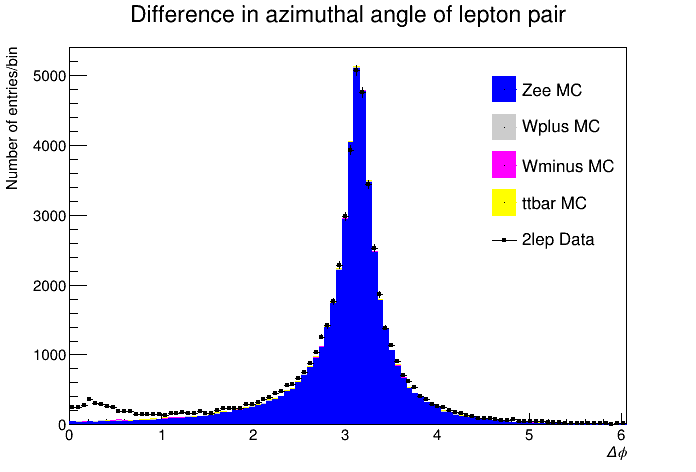
\includegraphics[width=\linewidth]{plots/25-02-2021/Zee-Stack_delta-phi_(min-cuts_2lep=ee)_25-02-21_09-25.png}
        (A)
    \end{minipage}\hfill
    \begin{minipage}{0.5\textwidth}
        \centering
        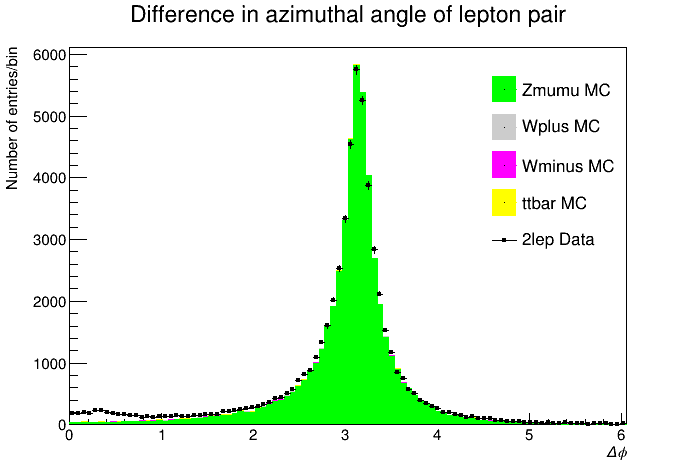
\includegraphics[width=\linewidth]{plots/25-02-2021/Zmumu-Stack_delta-phi_(min-cuts_2lep=mumu)_25-02-21_09-38.png}
        (B)
    \end{minipage}
    \caption{(A) Difference in azimuthal angle of ee pair produced. (B) Difference in azimuthal angle of $\mu\mu$ pair produced.  Cuts: }
    \label{fig:Zee-Stack_delta-phi_(min-cuts_2lep=ll)_25-02-21}
\end{figure}

\begin{lstlisting}
    lepCut ="(" + "(lep_charge[0] != lep_charge[1]) && (lep_type[0]==11 && lep_type[1]==11) && lep_n==2 && (inv_mass_Zll > 60e3)" + ")"
    
    t.SetAlias("inv_mass_Zll","sqrt(2*lep_pt[0]*lep_pt[1]*(cosh(lep_eta[0]-lep_eta[1])-cos(lep_phi[0]-lep_phi[1])))")
    t.Draw("abs(lep_phi[0] - lep_phi[1]) >> h_lep_delta_phi(100,0,6.3)", weighting + "*" + lepCut)
\end{lstlisting}

\begin{figure}[h!]
    \centering
    \begin{minipage}{0.5\textwidth}
        \centering
        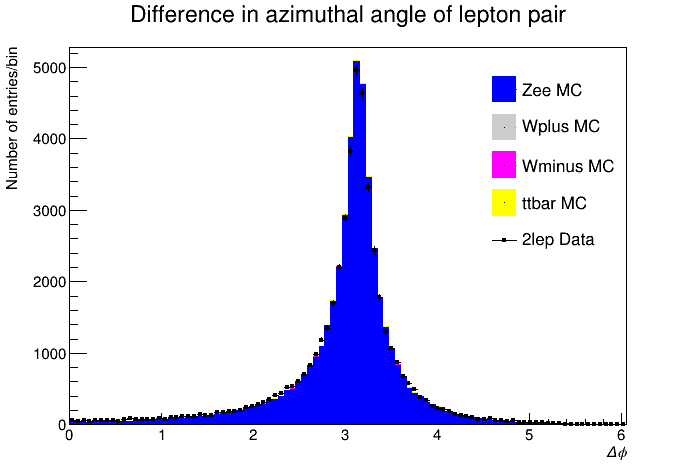
\includegraphics[width=\linewidth]{plots/25-02-2021/Zee-Stack-delta phi_(inv--mass-cut-lower-60GeV_2lep=ee)_25-02-21_09-30.png}
        (A)
    \end{minipage}\hfill
    \begin{minipage}{0.5\textwidth}
        \centering
        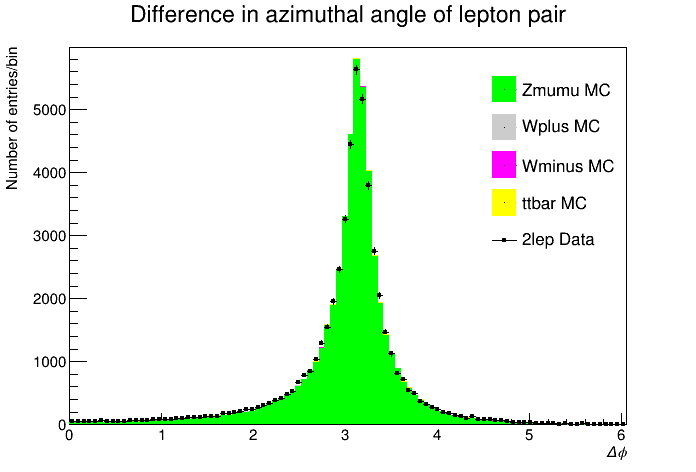
\includegraphics[width=\linewidth]{plots/25-02-2021/Zmumu-Stack-delta phi_(inv--mass-cut-lower-60GeV_2lep=mumu)_25-02-21_09-40.png}
        (B)
    \end{minipage}
    \caption{(A) (B).  Cuts: }
    \label{fig:}
\end{figure}

%%%%%%%%%%%%% 9:50 %%%%%%%%%%%%%
\subsubsection*{09:50}
Plotting the total transverse momentum ($p_T$) of two leptons of the same type and opposite charge being produced.


Cuts being used in Fig.\ref{fig:Zmumu-Stack_total-pt_(min-cut_2lep=ll)_25-02-21}
\begin{lstlisting}
    lepCut = "(" + "(lep_charge[0] != lep_charge[1]) && (lep_type[0] == 13 && lep_type[1] == 13) && lep_n==2" + ")"

    t.SetAlias("inv_mass_Zll","sqrt(2*lep_pt[0]*lep_pt[1]*(cosh(lep_eta[0]-lep_eta[1])-cos(lep_phi[0]-lep_phi[1])))")
    t.Draw("(lep_pt[0]+lep_pt[1]) >> h_lep_pt_total(200,0,500e3)", weighting + "*" + lepCut)
\end{lstlisting}

\begin{figure}[h!]
    \centering
    \begin{minipage}{0.5\textwidth}
        \centering
        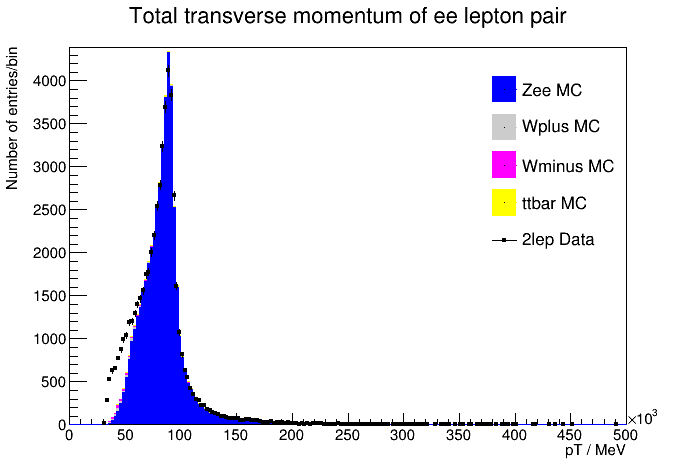
\includegraphics[width=\linewidth]{plots/25-02-2021/Zee-Stack_total-pt_(min-cut_2lep=e+e-)_25-02-21_09-50.png}
        (A)
    \end{minipage}\hfill
    \begin{minipage}{0.5\textwidth}
        \centering
        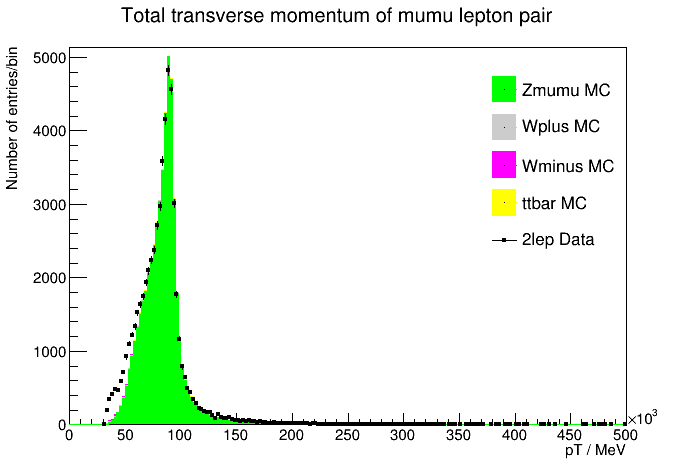
\includegraphics[width=\linewidth]{plots/25-02-2021/Zmumu-Stack_total-pt_(min-cut_2lep=mu+mu-)_25-02-21_09-50.png}
        (B)
    \end{minipage}
    \caption{(A) Total transverse momentum of e+e- pair. (B) Total transverse momentum of mu+mu- pair. Min cuts only: $lep_n==2$, opposite charge, specific type (e=11, mu=13)}
    \label{fig:Zmumu-Stack_total-pt_(min-cut_2lep=ll)_25-02-21}
\end{figure}

Cuts being used in Fig.\ref{fig:Zll-Stack_total-pt_(inv-mass-lower=60GeV_2lep=ll)_25-02-21}
\begin{lstlisting}
    lepCut = "(" + "(lep_charge[0] != lep_charge[1]) && (lep_type[0] == 13 && lep_type[1] == 13) && lep_n==2 && (inv_mass_Zll > 60000)" + ")"

    t.SetAlias("inv_mass_Zll","sqrt(2*lep_pt[0]*lep_pt[1]*(cosh(lep_eta[0]-lep_eta[1])-cos(lep_phi[0]-lep_phi[1])))")
    t.Draw("(lep_pt[0]+lep_pt[1]) >> h_lep_pt_total(200,0,500e3)", weighting + "*" + lepCut)
\end{lstlisting}

\begin{figure}[h!]
    \centering
    \begin{minipage}{0.5\textwidth}
        \centering
        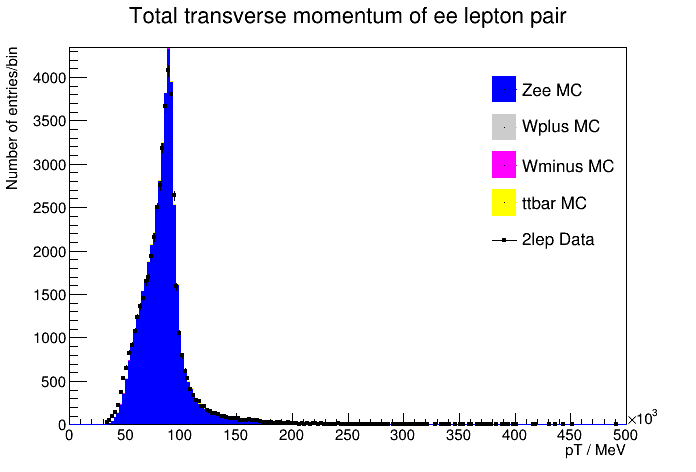
\includegraphics[width=\linewidth]{plots/25-02-2021/Zee-Stack_total-pt_(inv-mass-lower=60GeV_2lep=e+e-)_25-02-21_09-50.png}
        (A)
    \end{minipage}\hfill
    \begin{minipage}{0.5\textwidth}
        \centering
        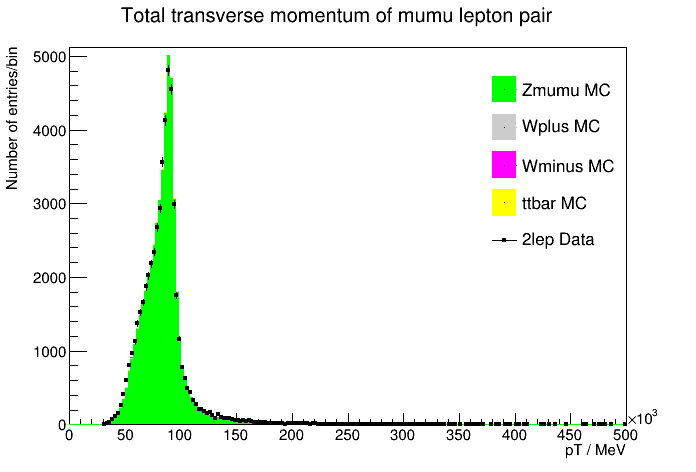
\includegraphics[width=\linewidth]{plots/25-02-2021/Zmumu-Stack_total-pt_(inv-mass-lower=60GeV_2lep=mu+mu-)_25-02-21_09-50.png}
        (B)
    \end{minipage}
    \caption{(A) Total transverse momentum of e+e- pair. (B) Total transverse momentum of mu+mu- pair. Only lower bound on invariant mass: $lep_n==2$, opposite charge, specific type (e=11, mu=13), and $m_{ll} > 60 GeV$ }
    \label{fig:Zll-Stack_total-pt_(inv-mass-lower=60GeV_2lep=ll)_25-02-21}
\end{figure}

%%%%%%%%%%%%% 9:50 %%%%%%%%%%%%%
\subsubsection*{09:50}
Plot the ptcone30.

Cuts for Fig.\ref{fig:Zll-stack_total-ptcone30_(min-cuts_2lep=ll)_25_02_21}
\begin{lstlisting}
# e=11, mu=13
lepCut = "(lep_charge[0] != lep_charge[1]) && (lep_type[0]==11 && lep_type[1]==11) && lep_n==2"

t.Draw("lep_ptcone30[0]+lep_ptcone30[1] >> h_lep_ptcone30(300,1e3,15e3)", weighting + "*" + lepCut)
\end{lstlisting}
\begin{figure}[h!]
    \centering
    \begin{minipage}{0.5\textwidth}
        \centering
        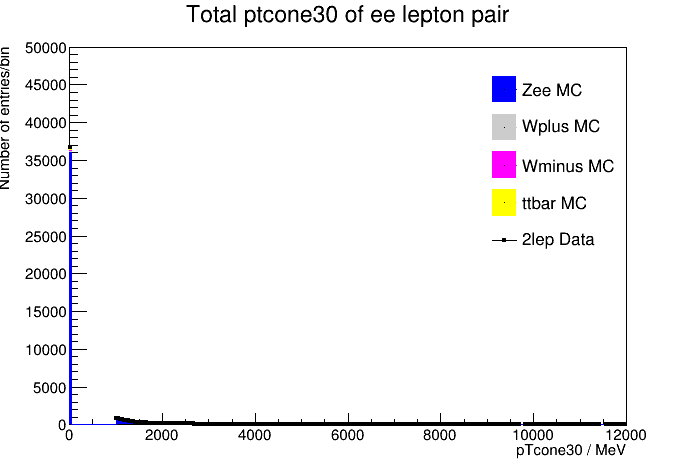
\includegraphics[width=\linewidth]{plots/25-02-2021/Zee-stack_total-ptcone30_(min-cuts_2lep=ee)_25_02_21_10-30_10-36.png}
        (A)
    \end{minipage}\hfill
    \begin{minipage}{0.5\textwidth}
        \centering
        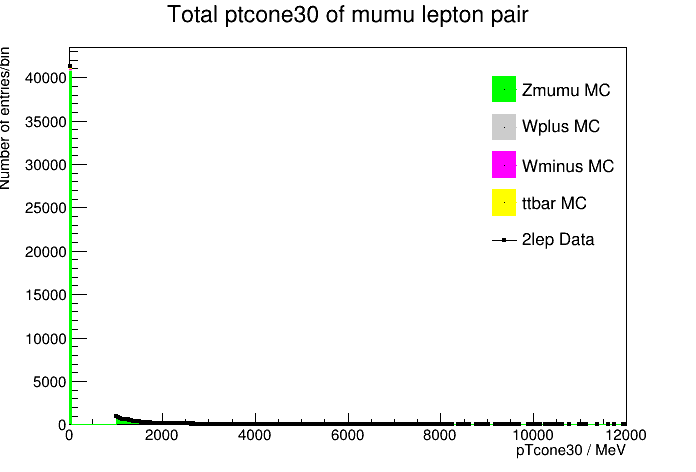
\includegraphics[width=\linewidth]{plots/25-02-2021/Zmumu-stack_total-ptcone30_(min-cuts_2lep=mumu)_25_02_21_10-30).png}
        (B)
    \end{minipage}
    \caption{(A) Total ptcone20 of ee pair. (B) Total ptcone20 of mumu pair.  Basic cuts: lep-n==2, same type, opposite charge.}
    \label{fig:Zll-stack_total-ptcone30_(min-cuts_2lep=ll)_25_02_21}
\end{figure}

Same as Fig.\ref{fig:Zll-stack_total-ptcone30_(min-cuts_2lep=ll)_25_02_21}, but different ptcone range to focus on $>$ 1 GeV. 
\\
Cuts for Fig.\ref{fig:Zmumu_Stack_total-ptcone30_(min-cuts_2lep=mumu)_25-02-21}
\begin{lstlisting}
    lepCut = "(lep_charge[0] != lep_charge[1]) && (lep_type[0]==11 && lep_type[1]==11) && lep_n==2"
    t.Draw("lep_ptcone30[0]+lep_ptcone30[1] >> h_lep_ptcone30(300,1e3,15e3)", weighting + "*" + lepCut)
\end{lstlisting}
\begin{figure}[h!]
    \centering
    \begin{minipage}{0.5\textwidth}
        \centering
        \includegraphics[width=\linewidth]{plots/}
        (A)
    \end{minipage}\hfill
    \begin{minipage}{0.5\textwidth}
        \centering
        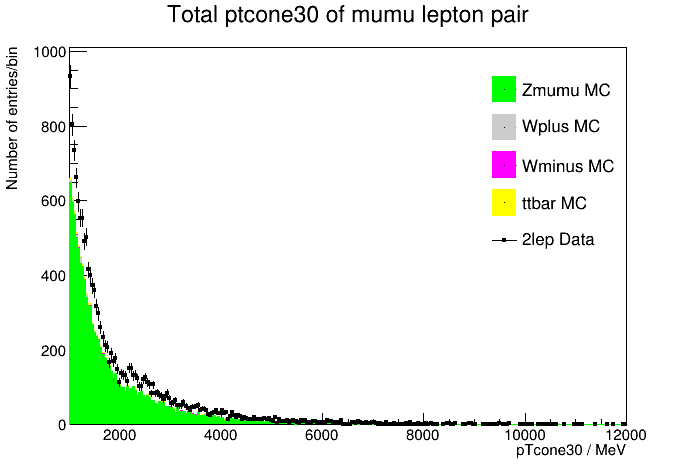
\includegraphics[width=\linewidth]{plots/25-02-2021/Zmumu_Stack_total-ptcone30_(min-cuts_2lep=mumu)_25-02-21_10-30.png}
        (B)
    \end{minipage}
    \caption{(A) Total ptcone20 of ee pair. (B) Total ptcone20 of mumu pair.  Basic cuts to include invariant mass: lep-n==2, same type, opposite charge, }
    \label{fig:Zmumu_Stack_total-ptcone30_(min-cuts_2lep=mumu)_25-02-21}
\end{figure}


Now applying invariant mass cut of lower bound of $>60 GeV$
Cuts for Fig.\ref{fig:Zee-stack_total-ptcone30_(inv-mass-lower=60GeV,2lep=ee)_25_02_21_10}
\begin{lstlisting}

\end{lstlisting}
\begin{figure}[h!]
    \centering
    \begin{minipage}{0.5\textwidth}
        \centering
        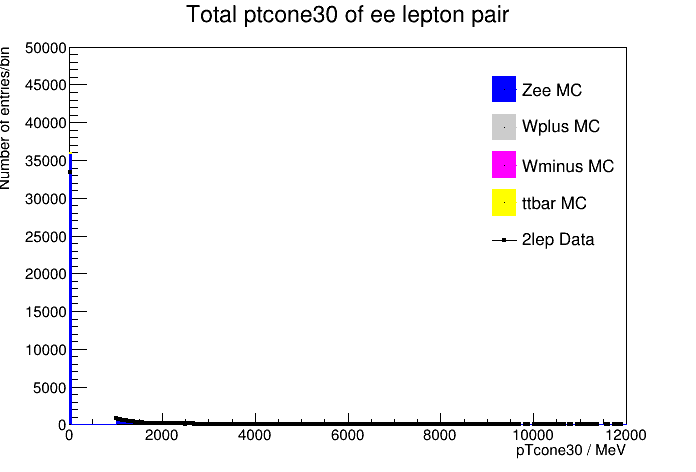
\includegraphics[width=\linewidth]{plots/25-02-2021/Zee-stack_total-ptcone30_(inv-mass-lower=60GeV,2lep=ee)_25_02_21_10-38).png}
        (A)
    \end{minipage}\hfill
    \begin{minipage}{0.5\textwidth}
        \centering
        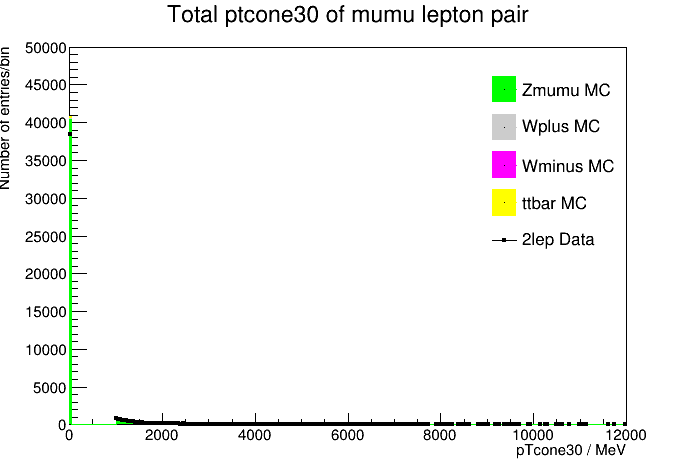
\includegraphics[width=\linewidth]{plots/25-02-2021/Zmumu-stack_total-ptcone30_(inv-mass-lower=60GeV,2lep=mumu)_25_02_21_10-30).png}
        (B)
    \end{minipage}
    \caption{(A) Total ptcone30 of ee pair being produced. (B) Total ptcone30 of mumu pair being produced. Cuts to include lower bound of invariant mass: lep-n==2, same type with opposite charge, invar-mass $>$ 60 GeV.}
    \label{fig:Zee-stack_total-ptcone30_(inv-mass-lower=60GeV,2lep=ee)_25_02_21_10}
\end{figure}



%%%%%%%%%%%%% 11:05 %%%%%%%%%%%%%
\subsubsection*{11:05}
Plot the etcone20.

Plotting the total ptcone20 with only the basic cuts. (same type opposite charge pair).  Fig.\ref{fig:Zll-stack_total-etcone_(min-cuts_2lep=l+l-)_25-02-21} as the cuts:
\begin{align}
# e=11, mu=13
lepCut ="(" + "(lep_charge[0] != lep_charge[1]) && (lep_type[0]== 13 && lep_type[1] == 13) && lep_n==2" + ")"    
    
t.SetAlias("inv_mass_Zll","sqrt(2*lep_pt[0]*lep_pt[1]*(cosh(lep_eta[0]-lep_eta[1])-cos(lep_phi[0]-lep_phi[1])))")
t.Draw("(lep_etcone20[0] + lep_etcone20[1]) >> h_lep_etcone20(200,-7e3,10e3)", weighting + "*" + lepCut)
\end{align}

\begin{figure}[h!]
    \centering
    \begin{minipage}{0.5\textwidth}
        \centering
        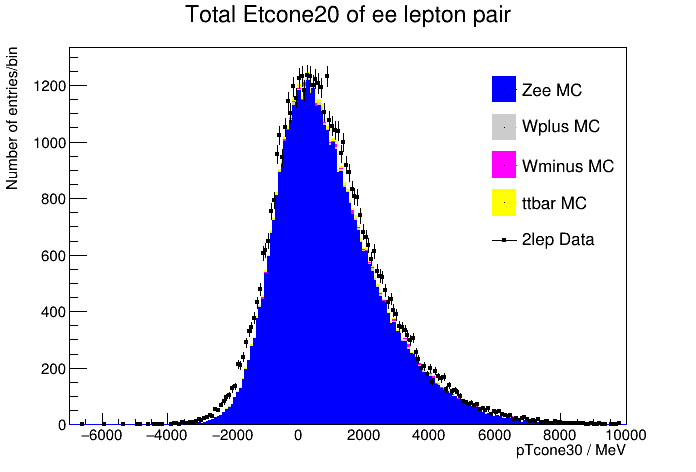
\includegraphics[width=\linewidth]{plots/25-02-2021/Zee-stack_total-etcone_(min-cuts_2lep=e+e-)_25-02-21_11-20.png}
        (A)
    \end{minipage}\hfill
    \begin{minipage}{0.5\textwidth}
        \centering
        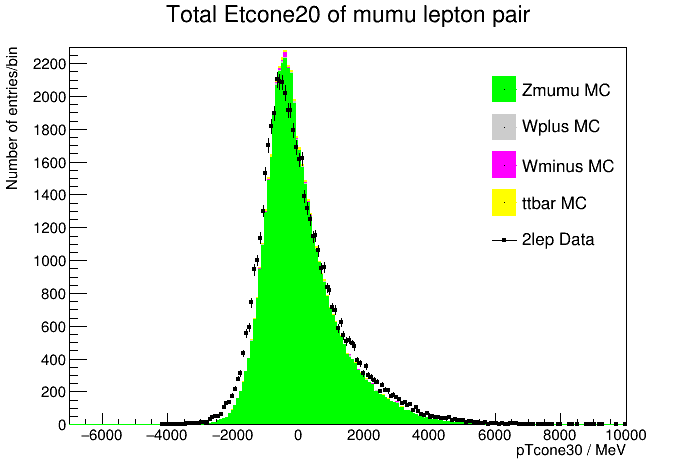
\includegraphics[width=\linewidth]{plots/25-02-2021/Zmumu-stack_total-etcone_(min-cuts_2lep=mu+mu-)_25-02-21_11-20.png}
        (B)
    \end{minipage}
    \caption{(A) Total etcone20 of ee pair produced (B) Total etcone20 of mumu pair produced. Basic Cuts: same type, opposite charged pair of leptons.}
    \label{fig:Zll-stack_total-etcone_(min-cuts_2lep=l+l-)_25-02-21}
\end{figure}



Applying the basic cuts along with the lower bound on the invariant mass ($m_{ll} > 60$ GeV).  Fig.\ref{} has the cuts:
\begin{lstlisting}
lepCut ="(" + "(lep_charge[0] != lep_charge[1]) && (lep_type[0]== 13 && lep_type[1] == 13) && lep_n==2 && inv_mass_Zll>60e3" + ")"    
    
    
    t.SetAlias("inv_mass_Zll","sqrt(2*lep_pt[0]*lep_pt[1]*(cosh(lep_eta[0]-lep_eta[1])-cos(lep_phi[0]-lep_phi[1])))")
    t.Draw("(lep_etcone20[0] + lep_etcone20[1]) >> h_lep_etcone20(200,-7e3,10e3)", weighting + "*" + lepCut)
\end{lstlisting}

\begin{figure}[h!]
    \centering
    \begin{minipage}{0.5\textwidth}
        \centering
        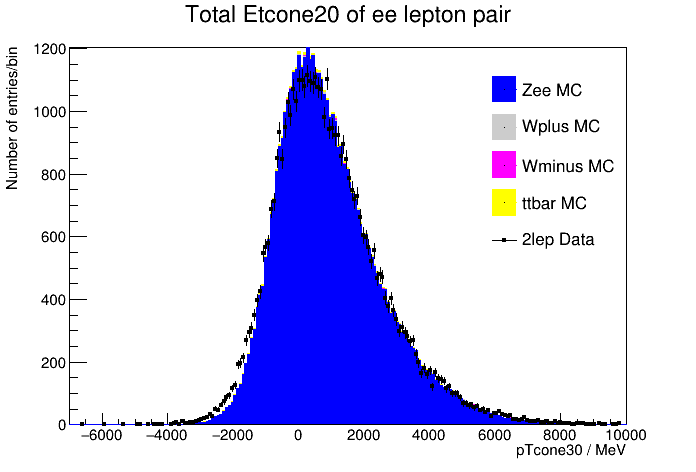
\includegraphics[width=\linewidth]{plots/25-02-2021/Zee-stack_total-etcone_(inv-mass-lower=60GeV_2lep=e+e-)_25-02-21_11-20.png}
        (A)
    \end{minipage}\hfill
    \begin{minipage}{0.5\textwidth}
        \centering
        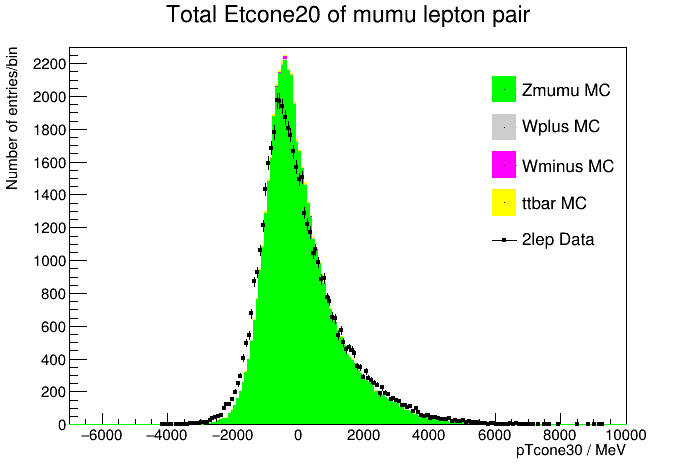
\includegraphics[width=\linewidth]{plots/25-02-2021/Zmumu-stack_total-etcone_(inv-mass-lower=60GeV_2lep=mu+mu-)_25-02-21_11-20).png}
        (B)
    \end{minipage}
    \caption{(A) Total etcone20 of ee pair produced (B) Total etcone20 of mumu pair produced. Cuts: invariant-mass $>$ 60 GeV, same type, opposite charged pair.}
    \label{fig:}
\end{figure}


%%%%%%%%%%%%% 11:30 %%%%%%%%%%%%% - Calculating the Zmumu cross section
\subsubsection*{11:30 - Lead BG - Calculating $\sigma(pp \rightarrow Z \rightarrow \mu\mu)$}
Calculating cross sections with varying cuts.
\\
The cross section: $\sigma (pp \rightarrow Z \rightarrow ee)$ is given by:
\begin{align}
    \sigma &= \frac{N^{selected} - N^{background}}{\epsilon \int L dt}
\end{align}
where
\begin{align}
     \epsilon &= \frac{\sum \text{weights for all MC events which pass selection cuts}}{\sum \text{weights for all events for that process}} 
\end{align}
\\
To start, calculate the cross section of $Z \rightarrow \mu\mu$ with cuts of:
\begin{itemize}
    \item $m_{ll} > 60$ GeV (lower bound on invaraint mass)
    \item Same lepton type 
    \item $lep_n == 2$ (number of leptons = 2)
    \item Opposite charge
\end{itemize}
Cross sections:
\begin{lstlisting}
t.SetAlias("inv_mass_Zll","sqrt(2*lep_pt[0]*lep_pt[1]*(cosh(lep_eta[0]-lep_eta[1])-cos(lep_phi[0]-lep_phi[1])))")
    
lepCut ="(" + "(lep_charge[0] != lep_charge[1]) && (lep_type[0]== 13 && lep_type[1] == 13) && lep_n==2 && inv_mass_Zll > 60e3" + ")"    
  
t.Draw("lep_n >> h_lep_n(3,-0.5,3.5)", weighting + "*" + lepCut)
\end{lstlisting}

Data sources: 
\begin{itemize}
    \item Background
    \subitem Wminus\_2lep, Wplus\_2lep, ttbar\_lep
    \item Source
    \subitem 2lep
    \item MC 
    \subitem Zmumu
\end{itemize}

\begin{align}
    N^{selected} &= 5288466
    \\
    N^{background}_{Wminus_2lep} &= 5904
    \\
    N^{background}_{Wplus_2lep} &= 6876
    \\
    N^{background}_{ttbar_lep} &= 3.063e4
    \\
    \epsilon &= \frac{5.153e6}{19631161.45} %3.063
\end{align}
Results:
\begin{align}
    \epsilon &= 0.2624908369850934
    \\
    \sigma (pp \rightarrow Z \rightarrow \mu\mu) &=  1.985479254338143e-09
\end{align}


%%%%%%%%%%%%% 12:12 %%%%%%%%%%%%% - Re-calculate the Zee cross section
\subsubsection*{12:12 - Calculating $\sigma(pp \rightarrow Z \rightarrow ee)$}
Data sources: 
\begin{itemize}
    \item Background
    \subitem Wminus\_2lep, Wplus\_2lep, ttbar\_lep
    \item Source
    \subitem 2lep
    \item MC 
    \subitem Zee
\end{itemize}

Cuts:
\begin{lstlisting}
t.SetAlias("inv_mass_Zll","sqrt(2*lep_pt[0]*lep_pt[1]*(cosh(lep_eta[0]-lep_eta[1])-cos(lep_phi[0]-lep_phi[1])))")
    
lepCut ="(" + "(lep_charge[0] != lep_charge[1]) && (lep_type[0]== 11 && lep_type[1] == 11) && lep_n==2 && inv_mass_Zll > 60e3" + ")"    
  
t.Draw("lep_n >> h_lep_n(3,-0.5,3.5)", weighting + "*" + lepCut)
\end{lstlisting}

Integral values
\begin{align}
    N^{selected} &= 4932622
    \\
    N^{background}_{Wminus_2lep} &= 6173
    \\
    N^{background}_{Wplus_2lep} &= 7268
    \\
    N^{background}_{ttbar_lep} &= 3.783e4
    \\
    \epsilon &= \frac{4.633e6}{19630128.89}
\end{align}

Results:
\begin{align}
    \epsilon &= 0.23601475191332785
    \\
    \sigma (pp \rightarrow Z \rightarrow ee) &= 2.0550872277842785e-09 b
\end{align}



%%%%%%%%%%%%% 14:00 %%%%%%%%%%%%% - Investigating Effect of transverse momentum lower bound cut on the cross section. 
\subsubsection*{14:00 - Lead BG}
Plot the total pt on a log y-scale to select a lower bound cut cut 

Cuts being used on Fig.\ref{fig:}

\begin{lstlisting}
# e=11, mu=13
lepCut = "(" + "(lep_charge[0] != lep_charge[1]) && (lep_type[0] == 11 && lep_type[1] == 11) && lep_n==2 && (inv_mass_Zll > 60e3)" + ")"

t.SetAlias("inv_mass_Zll","sqrt(2*lep_pt[0]*lep_pt[1]*(cosh(lep_eta[0]-lep_eta[1])-cos(lep_phi[0]-lep_phi[1])))")

t.Draw("(lep_pt[0]+lep_pt[1]) >> h_lep_pt_total(200,0,500e3)", weighting + "*" + lepCut)
\end{lstlisting}

\begin{figure}[h!]
    \centering
    \begin{minipage}{0.5\textwidth}
        \centering
        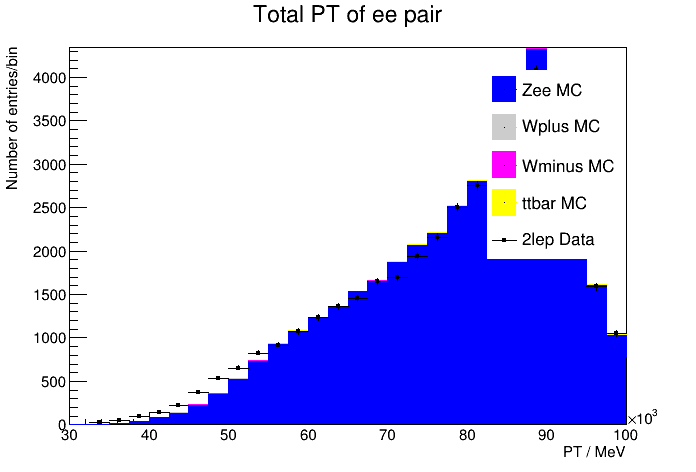
\includegraphics[width=\linewidth]{plots/25-02-2021/Zee-stack-(invar-mass-lower=60GeV,2lep=e+e-)-totalPt-lower-bound-justification_25-02-21_15-04.png}
        (A)
    \end{minipage}\hfill
    \begin{minipage}{0.5\textwidth}
        \centering
        \includegraphics[width=\linewidth]{plots/}
        (B)
    \end{minipage}
    \caption{(A) Total transverse momentum of electron pair (B) Total transverse momentum of muon pair. Cuts: }
    \label{fig:Zee-stack-(invar-mass-lower=60GeV,2lep=e+e-)-totalPt-lower-bound-justification_25-02-21}
\end{figure}

From Fig.\ref{fig:Zee-stack-(invar-mass-lower=60GeV,2lep=e+e-)-totalPt-lower-bound-justification_25-02-21}, choose a lower bound on PT of $55 GeV$.


%%%%%%%%%%%%% 15:00 %%%%%%%%%%%%% - Investigating Effect of transverse momentum lower bound cut on the cross section. 
\subsubsection*{15:00 - Calculating $\sigma(pp \rightarrow Z \rightarrow ee)$ lower cut on PT}
Calculating the cross section of... with the cuts :

\begin{lstlisting}
lepCut = "(" + "(lep_charge[0] != lep_charge[1]) && (lep_type[0] == 11 && lep_type[1] == 11) && lep_n==2 && (inv_mass_Zll > 60e3)" + ")"

t.SetAlias("inv_mass_Zll","sqrt(2*lep_pt[0]*lep_pt[1]*(cosh(lep_eta[0]-lep_eta[1])-cos(lep_phi[0]-lep_phi[1])))")

t.Draw("(lep_pt[0]+lep_pt[1]) >> h_lep_pt_total(200, 55e3,500e3)", weighting + "*" + lepCut)
\end{lstlisting}

Integral values
\begin{align}
    N^{selected} &= 4.66e6
    \\
    N^{background}_{Wminus\_2lep} &= 3006
    \\
    N^{background}_{Wplus\_2lep} &= 3256
    \\
    N^{background}_{ttbar\_lep} &= 3.687e4
    \\
    \epsilon &= \frac{4.472e6}{19630128.89}
\end{align}

Results:
\begin{align}
    \epsilon &= 0.2278130737225129
    \\
    \sigma (pp \rightarrow Z \rightarrow ee) &= 2.0137158391152733e-09 b
\end{align}


%%%%%%%%%%%%% 15:35 %%%%%%%%%%%%% - Investigating Effect of transverse momentum lower bound cut on Z->mumu cross section. 
\subsubsection*{15:35 - Calculating $\sigma(pp \rightarrow Z \rightarrow \mu\mu)$ lower cut on PT = 55 GeV}

\begin{lstlisting}
lepCut = "(" + "(lep_charge[0] != lep_charge[1]) && (lep_type[0] == 13 && lep_type[1] == 13) && lep_n==2 && (inv_mass_Zll > 60e3)" + ")"

t.SetAlias("inv_mass_Zll","sqrt(2*lep_pt[0]*lep_pt[1]*(cosh(lep_eta[0]-lep_eta[1])-cos(lep_phi[0]-lep_phi[1])))")

t.Draw("(lep_pt[0]+lep_pt[1]) >> h_lep_pt_total(200, 55e3,500e3)", weighting + "*" + lepCut)
\end{lstlisting}

Integral values
\begin{align}
    N^{selected} &= 5.061e6
    \\
    N^{background}_{Wminus\_2lep} &= 3620
    \\
    N^{background}_{Wplus\_2lep} &= 4241
    \\
    N^{background}_{ttbar\_lep} &= 2.985e4
    \\
    \epsilon &= \frac{4.912e6}{19631161.45}
\end{align}

Results:
\begin{align}
    \epsilon &= 0.25021443649733727
    \\
    \sigma (pp \rightarrow Z \rightarrow \mu\mu) &= 1.9948267037420005e-09 b
\end{align}


%%%%%%%%%%%%% 16:05 %%%%%%%%%%%%% - Increase transverse momentum lower bound cut on Z->mumu cross section to 80 GeV. 
\subsubsection*{15:35 - Calculating $\sigma(pp \rightarrow Z \rightarrow \mu\mu)$ lower cut on PT = 80 GeV}

\begin{lstlisting}
lepCut = "(" + "(lep_charge[0] != lep_charge[1]) && (lep_type[0] == 13 && lep_type[1] == 13) && lep_n==2 && (inv_mass_Zll > 60e3)" + ")"

t.SetAlias("inv_mass_Zll","sqrt(2*lep_pt[0]*lep_pt[1]*(cosh(lep_eta[0]-lep_eta[1])-cos(lep_phi[0]-lep_phi[1])))")

t.Draw("(lep_pt[0]+lep_pt[1]) >> h_lep_pt_total(200, 80e3,500e3)", weighting + "*" + lepCut)
\end{lstlisting}

Integral values. 
\begin{align}
    2lep &= 3.264e6
    \\
    Wminus\_2lep &= 1719
    \\
    Wplus\_2lep &= 2138
    \\
    ttbar\_lep &= 2.485e4
    \\
    Zmumu &= 3.142e6
\end{align}


\begin{align}
    N^{selected} &= 3.264e6
    \\
    N^{background}_{Wminus\_2lep} &= 1719
    \\
    N^{background}_{Wplus\_2lep} &= 2138
    \\
    N^{background}_{ttbar\_lep} &= 2.485e4
    \\
    \epsilon &= \frac{3.142e6}{19631161.45}
\end{align}

Results:
\begin{align}
    \epsilon &= 0.16005166113082933
    \\
    \sigma (pp \rightarrow Z \rightarrow ee) &= 2.0085507247902045e-09
\end{align}


%%%%%%%%%%%%% 16:22 %%%%%%%%%%%%% - Increase transverse momentum lower bound cut on Z->ee cross section to 80 GeV. 
\subsubsection*{15:35 - Calculating $\sigma(pp \rightarrow Z \rightarrow ee)$ lower cut on PT = 80 GeV}


\begin{lstlisting}
lepCut = "(" + "(lep_charge[0] != lep_charge[1]) && (lep_type[0] == 11 && lep_type[1] == 11) && lep_n==2 && (inv_mass_Zll > 60e3)" + ")"

t.SetAlias("inv_mass_Zll","sqrt(2*lep_pt[0]*lep_pt[1]*(cosh(lep_eta[0]-lep_eta[1])-cos(lep_phi[0]-lep_phi[1])))")

t.Draw("(lep_pt[0]+lep_pt[1]) >> h_lep_pt_total(200, 80e3,500e3)", weighting + "*" + lepCut)
\end{lstlisting}

Integral values. 
\begin{align}
    2lep &= 2.983e6
    \\
    Wminus\_2lep &= 1110
    \\
    Wplus\_2lep &= 1170
    \\
    ttbar\_lep &= 3.101e4
    \\
    Zee &= 2.838e6
\end{align}


\begin{align}
    N^{selected} &= 2.983e6
    \\
    N^{background}_{Wminus\_2lep} &= 1110
    \\
    N^{background}_{Wplus\_2lep} &= 1170
    \\
    N^{background}_{ttbar\_lep} &= 3.101e4
    \\
    \epsilon &= \frac{2.838e6}{19630128.89}
\end{align}

Results:
\begin{align}
    \epsilon &= 0.1445736814008255
    \\
    \sigma (pp \rightarrow Z \rightarrow ee) &= 2.0273066850004195e-09
\end{align}

\begin{tabular}{ c | c | c }
  \hline			
  var. & val. & uncert. \\
  
  $N^{selected}$ & - & - \\
  
  $N^{background}_{Wminus\_2lep}$ & - & - \\
  
  $N^{background}_{Wplus\_2lep}$ & - & - \\
  
  $N^{background}_{ttbar\_lep}$ & - & - \\
  
  $\epsilon_{num}$ & - & - \\
  
  $\epsilon_{den}$ & - & - \\
  \hline  
\end{tabular}




TODO:
\\
 - Plot sigma for different cuts on same plot.



%%%%%%%%%%%%%% 27/02/2020 %%%%%%%%%%%%%%%% 
\newpage
%%%%%%%%%%%%%% 27/02/2020 %%%%%%%%%%%%%%%% 
\subsection*{\textbf{27/02/2020}}
\subsubsection*{Days aims}
\begin{itemize}
    \item Finalize cuts to be made on $Z \rightarrow ee$ and $Z \rightarrow \mu\mu$
\end{itemize}

\subsubsection*{Day Summary}
\begin{itemize}
    \item Plotted total ptcone30
    \item Plotted total etcone20 
    \item Plotted PT of single leptons 
    \item Plotted the invaraint mass of ee and mumu pair 

    \item Cut on pT
    \subitem $Z \rightarrow ee$ = $36 GeV < p_T$
    \subitem $Z \rightarrow \mu\mu$ = $34 GeV < p_T$
    
    \item Cut on ptcone30 
    \subitem $Z \rightarrow ee$ = $ ptcone < 5.8 GeV$
    \subitem $Z \rightarrow \mu\mu$ = $ ptcone < 6.5 GeV$
    
    \item Cut on etcone20 
    \subitem $Z \rightarrow ee$ = $ -2 GeV < etcone < 6 GeV$
    \subitem $Z \rightarrow \mu\mu$ = $ -1.6 GeV < etcone < 5.25 GeV$
    
    \item Cut on invariant mass  
    \subitem $Z \rightarrow ee$ = $70 GeV < m_{ll} < 150 GeV$
    \subitem $Z \rightarrow \mu\mu$ = $60 GeV < m_{ll} < 150 GeV$
    
    \item Started to calculate cross sections for Z
\end{itemize}

%%%%%%%%%%%%% 9:00 %%%%%%%%%%%%%
\subsubsection*{09:00 - Lead BG}
Start by Plotting each variable, with and without a specific cut, and calculating the cross section for each.
\\
Make new notebook - \textit{DoubleHist} - to compare ATLAS data and a single MC data 

%%%%%%%%%%%%% 9:36 %%%%%%%%%%%%%
\subsubsection*{09:36}
Plot the ptcone30 for ee and $\mu\mu$ on sperate graphs on Fig.\ref{fig:All-stack-Zll-fast_(basic-cuts_2lep=ll_opp-c)_27-02-2021_09-50} with the cuts
\begin{lstlisting}
    # e=11, mu=13
    lepCut ="(" + "(lep_charge[0] != lep_charge[1]) && (lep_type[0]== 11 && lep_type[1] == 11) && lep_n==2" + ")"
    
    t.SetAlias("inv_mass_Zll","sqrt(2*lep_pt[0]*lep_pt[1]*(cosh(lep_eta[0]-lep_eta[1])-cos(lep_phi[0]-lep_phi[1])))")
    t.Draw("lep_ptcone30[0]+lep_ptcone30[1] >> h_lep_ptcone30(300,0,12e3)", weighting + "*" + lepCut)
\end{lstlisting}

\begin{figure}[h!]
    \centering
    \begin{minipage}{0.5\textwidth}
        \centering
        \includegraphics[width=\linewidth]{plots/27-02-2021/All-stack-Zee-fast_(basic-cuts_2lep=ee_opp-c)_27-02-2021_09-50.png}
        (A)
    \end{minipage}\hfill
    \begin{minipage}{0.5\textwidth}
        \centering
        \includegraphics[width=\linewidth]{plots/27-02-2021/2-Stack-Zee-2lep-fast_(basic-ee_opp-c)_27-02-21_10-00).png}
        (B)
    \end{minipage}
    \caption{(A) Total ptcone30 on a log-y graph for ee pair with simulated background (B) Total ptcone30 on a log-y graph for ee pair with simulated background. (only Basic) Cuts: lep-n=2, same type, opposite charge}
    \label{fig:All-stack-Zll-fast_(basic-cuts_2lep=ll_opp-c)_27-02-2021_09-50}
\end{figure}


From \ref{} the ATLAS data follows the MC. data well for 


\subsubsection*{10:05}
Apply the Invariant mass cut the the ptcone log plot to see if that changes for ee


\begin{figure}[h!]
    \centering
    \begin{minipage}{0.5\textwidth}
        \centering
        \includegraphics[width=\linewidth]{plots/27-02-2021/}
        (A)
    \end{minipage}\hfill
    \begin{minipage}{0.5\textwidth}
        \centering
        \includegraphics[width=\linewidth]{plots/27-02-2021/2-Stack-Zee-2lep-fast_(basic-and_invarmass-lower=60GeV)_27-02-21_10-10).png}
        (B)
    \end{minipage}
    \caption{(A)  (B) Total ptcone30 of ee pair for ATLAS and Zmumu MC. Cuts: invar-mass-lower=60GeV, pair of mu with opposite charge.}
    \label{}
\end{figure}

%%%%%%%%%%%%% 10:17 %%%%%%%%%%%%%
\subsubsection*{10:17}
Plot the total ptone30 for mumu on a log-y plot
with the cuts used in Fig.\ref{fig:stack-Zmumu-fast_(invar-mass-lower=60GeV)_27-02-21_10-19} to include a lower bound on the invariant mass:
\begin{lstlisting}
lepCut ="(" + "(lep_charge[0] != lep_charge[1]) && (lep_type[0]== 13 && lep_type[1] == 13) && lep_n==2 " + ")"
    
t.SetAlias("inv_mass_Zll","sqrt(2*lep_pt[0]*lep_pt[1]*(cosh(lep_eta[0]-lep_eta[1])-cos(lep_phi[0]-lep_phi[1])))")

t.Draw("lep_ptcone30[0]+lep_ptcone30[1] >> h_lep_ptcone30(100,0,12e3)", weighting + "*" + lepCut)
\end{lstlisting}
% invar mas 
\begin{figure}[h!]
    \centering
    \begin{minipage}{0.5\textwidth}
        \centering
        \includegraphics[width=\linewidth]{plots/27-02-2021/}
        (A)
    \end{minipage}\hfill
    \begin{minipage}{0.5\textwidth}
        \centering
        \includegraphics[width=\linewidth]{plots/27-02-2021/2-stack-Zmumu-fast_(invar-mass-lower=60GeV)_27-02-21_10-19.png}
        (B)
    \end{minipage}
    \caption{(A)  (B) ptcone30 of Z -> mumu for the ATLAS and Zmumu MC data. Cuts: invar-mass-lower=60GeV, with basic cuts of mu pair with opposite charge.}
    \label{fig:stack-Zmumu-fast_(invar-mass-lower=60GeV)_27-02-21_10-19}
\end{figure}

%%%%%%%%%%%%% 10:27 %%%%%%%%%%%%%
\subsubsection*{10:27}
Plot total ptcone30 for mu pair without invar-mass-lower=60GeV cut.
\\
Cuts using for Fig.\ref{fig:stack-Zmumu-fast_(basics_mu-pair_opp-c)_27-02-21_10-27}
\begin{lstlisting}
lepCut ="(" + "(lep_charge[0] != lep_charge[1]) && (lep_type[0]== 13 && lep_type[1] == 13) && lep_n==2 " + ")"
    
t.SetAlias("inv_mass_Zll","sqrt(2*lep_pt[0]*lep_pt[1]*(cosh(lep_eta[0]-lep_eta[1])-cos(lep_phi[0]-lep_phi[1])))")

t.Draw("lep_ptcone30[0]+lep_ptcone30[1] >> h_lep_ptcone30(100,0,12e3)", weighting + "*" + lepCut)
\end{lstlisting}

\begin{figure}[h!]
    \centering
    \begin{minipage}{0.5\textwidth}
        \centering
        \includegraphics[width=\linewidth]{plots/27-02-2021/}
        (A)
    \end{minipage}\hfill
    \begin{minipage}{0.5\textwidth}
        \centering
        \includegraphics[width=\linewidth]{plots/27-02-2021/2-stack-Zmumu-fast_(basics_mu-pair_opp-c)_27-02-21_10-27.png}
        (B)
    \end{minipage}
    \caption{(A)  (B) Total ptcone30 of $Z -> \mu\mu$ for the ATLAS and Zmumu MC data. With basic cuts of mu pair with opposite charge.}
    \label{fig:stack-Zmumu-fast_(basics_mu-pair_opp-c)_27-02-21_10-27}
\end{figure}


%%%%%%%%%%%%% 10:30 %%%%%%%%%%%%%
\subsubsection*{10:30}
Plotting the total etcone20 of ee pair with only basic cuts on log-y plot.
\\
Cuts used in Fig.\ref{}
\begin{lstlisting}
lepCut ="(" + "(lep_charge[0] != lep_charge[1]) && (lep_type[0]== 11 && lep_type[1] == 11) && lep_n==2" + ")"    
    
t.SetAlias("inv_mass_Zll","sqrt(2*lep_pt[0]*lep_pt[1]*(cosh(lep_eta[0]-lep_eta[1])-cos(lep_phi[0]-lep_phi[1])))")

t.Draw("(lep_etcone20[0] + lep_etcone20[1]) >> h_lep_etcone20(100,-7e3,14e3)", weighting + "*" + lepCut)
\end{lstlisting}
\begin{figure}[h!]
    \centering
    \begin{minipage}{0.5\textwidth}
        \centering
        \includegraphics[width=\linewidth]{plots/27-02-2021/}
        (A)
    \end{minipage}\hfill
    \begin{minipage}{0.5\textwidth}
        \centering
        \includegraphics[width=\linewidth]{plots/27-02-2021/2-Stack-Zee-fast_total-etcone_(basic-cuts_ee-pair-opp-c)_27-02-21_10-35.png}
        (B)
    \end{minipage}
    \caption{(A)  (B) Total etcone20 of ee pair for ATLAS and Zee MC. Cuts: (only basic) ee pair with opposite charge.}
    \label{}
\end{figure}

%%%%%%%%%%%%% 10:39 %%%%%%%%%%%%%
\subsubsection*{10:39}
Plotting the single etcone20 of one of the particle of the ee pair with only basic cuts on log-y plot.
\\
Cuts used in Fig.\ref{fig:2-Stack-Zee-fast_etcone[0]_(basic-ee_opp-c)_27-02-21_10-39}
\begin{lstlisting}
lepCut ="(" + "(lep_charge[0] != lep_charge[1]) && (lep_type[0]== 11 && lep_type[1] == 11) && lep_n==2" + ")"    
    
t.SetAlias("inv_mass_Zll","sqrt(2*lep_pt[0]*lep_pt[1]*(cosh(lep_eta[0]-lep_eta[1])-cos(lep_phi[0]-lep_phi[1])))")

t.Draw("lep_etcone20[0] >> h_lep_etcone20(100,-7e3,14e3)", weighting + "*" + lepCut)
\end{lstlisting}

\begin{figure}[h!]
    \centering
    \begin{minipage}{0.5\textwidth}
        \centering
        \includegraphics[width=\linewidth]{plots/27-02-2021/}
        (A)
    \end{minipage}\hfill
    \begin{minipage}{0.5\textwidth}
        \centering
        \includegraphics[width=\linewidth]{plots/27-02-2021/2-Stack-Zee-fast_etcone[0]_(basic-ee_opp-c)_27-02-21_10-39.png}
        (B)
    \end{minipage}
    \caption{(A)  (B) Single etcone20 of a single particle for ee pair.  Cuts: (only basic) ee pair with opposite charge}
    \label{fig:2-Stack-Zee-fast_etcone[0]_(basic-ee_opp-c)_27-02-21_10-39}
\end{figure}

%%%%%%%%%%%%% 10:50 %%%%%%%%%%%%% - etcone20 (single muon) (log-y)
\subsubsection*{10:50 - etcone20 of single muon (log-y)}
Potting the etcone20 of a single muon of a mumu pair on a log-y plot using only the basic cuts (mumu pair with opposite charge).
\\
The cuts used in Fig.\ref{fig:Stack-Zmumu-fast_single-etcone_(basic-cuts_2mumu-pair-opp-c)_27-02-21_10-50}
\begin{lstlisting}
lepCut ="(" + "(lep_charge[0] != lep_charge[1]) && (lep_type[0]== 13 && lep_type[1] == 13) && lep_n==2" + ")"    
    
t.SetAlias("inv_mass_Zll","sqrt(2*lep_pt[0]*lep_pt[1]*(cosh(lep_eta[0]-lep_eta[1])-cos(lep_phi[0]-lep_phi[1])))")

t.Draw("lep_etcone20[0] >> h_lep_etcone20(100,-7e3,14e3)", weighting + "*" + lepCut)
\end{lstlisting}

\begin{figure}[h!]
    \centering
    \begin{minipage}{0.5\textwidth}
        \centering
        \includegraphics[width=\linewidth]{plots/27-02-2021/}
        (A)
    \end{minipage}\hfill
    \begin{minipage}{0.5\textwidth}
        \centering
        \includegraphics[width=\linewidth]{plots/27-02-2021/2-stack-Zmumu-fast_single-etcone_(basic-cuts_2mumu-pair-opp-c)_27-02-21_10-50.png}
        (B)
    \end{minipage}
    \caption{(A)  (B) etcone20 of single muon for both ATLAS and Zmumu.  Cuts: (basic only) }
    \label{fig:Stack-Zmumu-fast_single-etcone_(basic-cuts_2mumu-pair-opp-c)_27-02-21_10-50}
\end{figure}

%%%%%%%%%%%%% 10:57 %%%%%%%%%%%%% - Difference in etcone (log-y)
\subsubsection*{10:57 - Difference in etcone}
Plotting the difference in etcone20 for mumu with only the basic cuts being used in Fig.\ref{fig:Stack-Zmumu-fast_etcone-difference_log-y_(basic-cuts_2lep=mumu_opp-c)_27-02-21_10-57}:
\begin{lstlisting}
lepCut ="(" + "(lep_charge[0] != lep_charge[1]) && (lep_type[0]== 13 && lep_type[1] == 13) && lep_n==2" + ")"    
    
t.SetAlias("inv_mass_Zll","sqrt(2*lep_pt[0]*lep_pt[1]*(cosh(lep_eta[0]-lep_eta[1])-cos(lep_phi[0]-lep_phi[1])))")
    
t.Draw("abs(lep_etcone20[0]-lep_etcone20[1]) >> h_lep_etcone20(100,-7e3,14e3)", weighting + "*" + lepCut)
\end{lstlisting}

\begin{figure}[h!]
    \centering
    \begin{minipage}{0.5\textwidth}
        \centering
        \includegraphics[width=\linewidth]{plots/27-02-2021/All-Stack-Zmumu-fast_etcone-difference_log-y_(basic-cuts_2lep=mumu_opp-c)_27-02-21_10-57.png}
        (A)
    \end{minipage}\hfill
    \begin{minipage}{0.5\textwidth}
        \centering
        \includegraphics[width=\linewidth]{plots/27-02-2021/2-Stack-Zmumu-fast_etcone-difference_log-y_(basic-cuts_2lep=mumu_opp-c)_27-02-21_10-57.png}
        (B)
    \end{minipage}
    \caption{(A) The absolute difference in etcone20 for ATLAS, MC and MC background. (B) The absolute difference in etcone20 for $Z \rightarrow \mu\mu$ using both ATLAS and MC data.  Cuts: (only basic) mumu pair with opposite charge}
    \label{fig:Stack-Zmumu-fast_etcone-difference_log-y_(basic-cuts_2lep=mumu_opp-c)_27-02-21_10-57}
\end{figure}


%%%%%%%%%%%%% 11:05 %%%%%%%%%%%%% - Difference in etcone
\subsubsection*{11:05 - Difference in etcone}
Plotting the absolute difference in etcone20 for mumu pair of opposite charge.
\\
Cuts used in Fig.\ref{fig:Stack-Zmumu-fast_etcone-difference_(basic-cuts_2lep=mumu_opp-c)_27-02-21_11-05}:
\begin{lstlisting}
lepCut ="(" + "(lep_charge[0] != lep_charge[1]) && (lep_type[0]== 13 && lep_type[1] == 13) && lep_n==2" + ")"    
    
t.SetAlias("inv_mass_Zll","sqrt(2*lep_pt[0]*lep_pt[1]*(cosh(lep_eta[0]-lep_eta[1])-cos(lep_phi[0]-lep_phi[1])))")
   
t.Draw("abs(lep_etcone20[0]-lep_etcone20[1]) >> h_lep_etcone20(100,-7e3,14e3)", weighting + "*" + lepCut)
\end{lstlisting}

\begin{figure}[h!]
    \centering
    \begin{minipage}{0.5\textwidth}
        \centering
        \includegraphics[width=\linewidth]{plots/27-02-2021/All-Stack-Zmumu-fast_etcone-difference_(basic-cuts_2lep=mumu_opp-c)_27-02-21_11-05.png}
        (A)
    \end{minipage}\hfill
    \begin{minipage}{0.5\textwidth}
        \centering
        \includegraphics[width=\linewidth]{plots/27-02-2021/2-Stack-Zmumu-fast_etcone-difference_(basic-cuts_2lep=mumu_opp-c)_27-02-21_11-05.png}
        (B)
    \end{minipage}
    \caption{(A) The absolute difference in etcone20 for ATLAS, MC and MC background. (B) The absolute difference in etcone20 for $Z \rightarrow \mu\mu$.  Cuts: (only basic) mumu pair with opposite charge }
    \label{fig:Stack-Zmumu-fast_etcone-difference_(basic-cuts_2lep=mumu_opp-c)_27-02-21_11-05}
\end{figure}



%%%%%%%%%%%%% 11:30 %%%%%%%%%%%%% - ptcone30 for single electron from ee pair (log-y
\subsubsection*{11:30 - ptcone30 for single e from ee pair (log-y)}
PLotting the ptcone30 for a single electron on a log-y plot.
\\
Cuts used in Fig.\ref{fig:stack-Zee-fast_ptcone30-single_log-y_(basics_2lep=ee-opp-c)_27-02-21_11-30}:
\begin{lstlisting}
....
\end{lstlisting}
\begin{figure}[h!]
    \centering
    \begin{minipage}{0.5\textwidth}
        \centering
        \includegraphics[width=\linewidth]{plots/27-02-2021/}
        (A)
    \end{minipage}\hfill
    \begin{minipage}{0.5\textwidth}
        \centering
        \includegraphics[width=\linewidth]{plots/27-02-2021/2-stack-Zee-fast_ptcone30-single_log-y_(basics_2lep=ee-opp-c)_27-02-21_11-30.png}
        (B)
    \end{minipage}
    \caption{(A)  (B) ptcone30 of single electron from ee pair using the ATLAS and MC Zee data. Cuts: (basic) ee pair with oppsoite charge.}
    \label{fig:stack-Zee-fast_ptcone30-single_log-y_(basics_2lep=ee-opp-c)_27-02-21_11-30}
\end{figure}

%%%%%%%%%%%%% 11:32 %%%%%%%%%%%%% -  ptcone for single muon of mumu pair (log-y
\subsubsection*{11:32 - ptcone30 for single muon in mumu pair (log-y)}
PLotting the ptcone30 for a single muon on a log-y plot.
\\
Cuts using in Fig.\ref{fig:stack-Zmumu-fast_ptcone30-single_log-y_(basics_2lep=mumu-opp-c)_27-02-21_11-30}:
\begin{lstlisting}
....
\end{lstlisting}
\begin{figure}[h!]
    \centering
    \begin{minipage}{0.5\textwidth}
        \centering
        \includegraphics[width=\linewidth]{plots/27-02-2021/}
        (A)
    \end{minipage}\hfill
    \begin{minipage}{0.5\textwidth}
        \centering
        \includegraphics[width=\linewidth]{plots/27-02-2021/2-stack-Zmumu-fast_ptcone30-single_log-y_(basics_2lep=mumu-opp-c)_27-02-21_11-30.png}
        (B)
    \end{minipage}
    \caption{(A)  (B) ptcone30 of single muon from mumu pair using the ATLAS and MC Zmumu data. Cuts: (basic) mumu pair with oppsoite charge. }
    \label{fig:stack-Zmumu-fast_ptcone30-single_log-y_(basics_2lep=mumu-opp-c)_27-02-21_11-30}
\end{figure}

%%%%%%%%%%%%% 11:40 %%%%%%%%%%%%% - PT single e (log-y)
\subsubsection*{11:40 - PT single e (log-y)}
Plotting the transverse momentum for single electron from ee pair with opposite charge on log-y.
\\
Cuts using in Fig.\ref{fig:Stack-Zee-fast_PT-single_log-y_(basic-cuts_2lep=ee_opp-c)_27-02-21_11-40}:
\begin{lstlisting}
lepCut = "(" + "(lep_charge[0] != lep_charge[1]) && (lep_type[0] == 11 && lep_type[1] == 11) && lep_n==2" + ")"

t.SetAlias("inv_mass_Zll","sqrt(2*lep_pt[0]*lep_pt[1]*(cosh(lep_eta[0]-lep_eta[1])-cos(lep_phi[0]-lep_phi[1])))")

t.Draw("lep_pt[0] >> h_lep_pt_total(100, 0,100e3)", weighting + "*" + lepCut)
\end{lstlisting}

\begin{figure}[h!]
    \centering
    \begin{minipage}{0.5\textwidth}
        \centering
        \includegraphics[width=\linewidth]{plots/27-02-2021/}
        (A)
    \end{minipage}\hfill
    \begin{minipage}{0.5\textwidth}
        \centering
        \includegraphics[width=\linewidth]{plots/27-02-2021/2-Stack-Zee-fast_PT-single_log-y_(basic-cuts_2lep=ee_opp-c)_27-02-21_11-40.png}
        (B)
    \end{minipage}
    \caption{(A)  (B) Transverse momentum of a single electron from a ee pair using the ATLAS and MC Zee data.  Cuts: (basic only). ee pair with opposite charge.}
    \label{fig:Stack-Zee-fast_PT-single_log-y_(basic-cuts_2lep=ee_opp-c)_27-02-21_11-40}
\end{figure}


%%%%%%%%%%%%% 11:50 %%%%%%%%%%%%% - PT single mu (log-y)
\subsubsection*{11:50 - PT single mu (log-y)}
Plotting the transverse momentum (PT) of single muon from a mumu pair with opposite charge on a log-y plot.
\\
Cuts used in Fig.\ref{}:
\begin{lstlisting}
lepCut = "(" + "(lep_charge[0] != lep_charge[1]) && (lep_type[0] == 13 && lep_type[1] == 13) && lep_n==2" + ")"

t.SetAlias("inv_mass_Zll","sqrt(2*lep_pt[0]*lep_pt[1]*(cosh(lep_eta[0]-lep_eta[1])-cos(lep_phi[0]-lep_phi[1])))")

t.Draw("lep_pt[0] >> h_lep_pt_total(100, 0,100e3)", weighting + "*" + lepCut)
\end{lstlisting}

% 2-Statck-Zmumu-fast_PT-single_log-y_(basic-cuts_2lep=mumu_opp-c)_27-02-21_11-50.png

\begin{figure}[h!]
    \centering
    \begin{minipage}{0.5\textwidth}
        \centering
        \includegraphics[width=\linewidth]{plots/27-02-2021/}
        (A)
    \end{minipage}\hfill
    \begin{minipage}{0.5\textwidth}
        \centering
        \includegraphics[width=\linewidth]{plots/27-02-2021/2-Statck-Zmumu-fast_PT-single_log-y_(basic-cuts_2lep=mumu_opp-c)_27-02-21_11-50.png}
        (B)
    \end{minipage}
    \caption{(A)  (B) Transverse momentum of a single muon shown for ATLAS and Zmumu MC data.  Cuts: (Basic) mumu pair with opposite charge.}
    \label{}
\end{figure}


%%%%%%%%%%%%% 12:00 %%%%%%%%%%%%% - PT single mu (non-log)
\subsubsection*{12:00 - PT single mu}
% (B) 2-stack-Zmumu-fast_PT-single_(basic_2lep=mumu-opp-c)_27-02-21_12-00.png
Plotting the transverse momentum of single muon of mumu pair of opposite charge on a log-y plot.
\\
Cuts used in Fig.\ref{fig:2-stack-Zmumu-fast_PT-single_(basic_2lep=mumu-opp-c)_27-02-21_12-00}:
\begin{lstlisting}
lepCut = "(" + "(lep_charge[0] != lep_charge[1]) && (lep_type[0] == 11 && lep_type[1] == 11) && lep_n==2" + ")"

t.SetAlias("inv_mass_Zll","sqrt(2*lep_pt[0]*lep_pt[1]*(cosh(lep_eta[0]-lep_eta[1])-cos(lep_phi[0]-lep_phi[1])))")

t.Draw("lep_pt[0] >> h_lep_pt_total(100, 0,100e3)", weighting + "*" + lepCut)
\end{lstlisting}

\begin{figure}[h!]
    \centering
    \begin{minipage}{0.5\textwidth}
        \centering
        \includegraphics[width=\linewidth]{plots/27-02-2021/}
        (A)
    \end{minipage}\hfill
    \begin{minipage}{0.5\textwidth}
        \centering
        \includegraphics[width=\linewidth]{plots/27-02-2021/2-stack-Zmumu-fast_PT-single_(basic_2lep=mumu-opp-c)_27-02-21_12-00.png}
        (B)
    \end{minipage}
    \caption{(A)  (B) Transverse momentum of single muon using ATLAS and Zmumu MC data.  Cuts: (basic) muon pair of opposite charge.}
    \label{fig:2-stack-Zmumu-fast_PT-single_(basic_2lep=mumu-opp-c)_27-02-21_12-00}
\end{figure}

%%%%%%%%%%%%% 12:03 %%%%%%%%%%%%% - PT single electron (non-log)
\subsubsection*{12:03 - PT single electron}
% (B) 2-stack-fast_PT-single_(basic_2lep=ee-opp-c)_27-02-21_12-03.png
Plotting the transverse momentum of single electron of ee pair of opposite charge (standard plot).
\\
Cuts used in Fig.\ref{fig:stack-fast_PT-single_(basic_2lep=ee-opp-c)_27-02-21_12-03}
\begin{lstlisting}
lepCut = "(" + "(lep_charge[0] != lep_charge[1]) && (lep_type[0] == 11 && lep_type[1] == 11) && lep_n==2" + ")"

t.SetAlias("inv_mass_Zll","sqrt(2*lep_pt[0]*lep_pt[1]*(cosh(lep_eta[0]-lep_eta[1])-cos(lep_phi[0]-lep_phi[1])))")

t.Draw("lep_pt[0] >> h_lep_pt_total(100, 0,100e3)", weighting + "*" + lepCut)
\end{lstlisting}

\begin{figure}[h!]
    \centering
    \begin{minipage}{0.5\textwidth}
        \centering
        \includegraphics[width=\linewidth]{plots/27-02-2021/}
        (A)
    \end{minipage}\hfill
    \begin{minipage}{0.5\textwidth}
        \centering
        \includegraphics[width=\linewidth]{plots/27-02-2021/2-stack-fast_PT-single_(basic_2lep=ee-opp-c)_27-02-21_12-03.png}
        (B)
    \end{minipage}
    \caption{(A)  (B) Transverse momentum of single electron using both ATLAS and Zee MC data.  Cuts: (Basic) ee pair with opposite charge.}
    \label{fig:stack-fast_PT-single_(basic_2lep=ee-opp-c)_27-02-21_12-03}
\end{figure}

%%%%%%%%%%%%% 12:05 %%%%%%%%%%%%% - Invariant mass ($m_{ee}$) (log-y)
\subsubsection*{12:05 - Invariant mass ($m_{ee}$) (log-y)}
% (B) 2-Stack-Zee-fast_mll_log-y_0-200GeV_(basic_2lep=ee_opp-c)_27-02-21_12-05.png
Plotting the invariant mass of ee pair of opposite charge (log-y plot).
\\
Cuts used in Fig.\ref{fig:Stack-Zee-fast_mll_log-y_0-200GeV_(basic_2lep=ee_opp-c)_27-02-21_12-05}
\begin{lstlisting}
t.SetAlias("inv_mass_Zll","sqrt(2*lep_pt[0]*lep_pt[1]*(cosh(lep_eta[0]-lep_eta[1])-cos(lep_phi[0]-lep_phi[1])))")

# oposite charged pair of leptons (lep_n == 2)
lepCut = "(" + "(lep_charge[0] != lep_charge[1]) && lep_n==2 && lep_type[0]==11 && lep_type[1]== 11" + ")"
    
t.Draw("inv_mass_Zll >> h_inv_mass_Zll(100,0e3,200e3)", weighting + "*" + lepCut) 
\end{lstlisting}

\begin{figure}[h!]
    \centering
    \begin{minipage}{0.5\textwidth}
        \centering
        \includegraphics[width=\linewidth]{plots/27-02-2021/}
        (A)
    \end{minipage}\hfill
    \begin{minipage}{0.5\textwidth}
        \centering
        \includegraphics[width=\linewidth]{plots/27-02-2021/2-Stack-Zee-fast_mll_log-y_0-200GeV_(basic_2lep=ee_opp-c)_27-02-21_12-05.png}
        (B)
    \end{minipage}
    \caption{(A)  (B) Invariant mass of ee pair using ATLAS and Zee MC data.  Cuts: (basic) ee pair with opposite charge.}
    \label{fig:Stack-Zee-fast_mll_log-y_0-200GeV_(basic_2lep=ee_opp-c)_27-02-21_12-05}
\end{figure}

%%%%%%%%%%%%% 12:07 %%%%%%%%%%%%% - Invariant mass ($m_{\mu\mu}$) (log-y)
\subsubsection*{12:07 - Invariant mass ($m_{\mu\mu}$) (log-y)}
% (B) 2-Stack-Zmumu-fast_mll_log-y_0-200GeV_(basic_2lep=mumu_opp-c)_27-02-21_12-07.png
Plotting the invariant mass of mumu pair of opposite charge (log-y plot) with basic cuts (mumu pair with oppsite charge).
\\
Cuts used in Fig.\ref{fig:Stack-Zmumu-fast_mll_log-y_0-200GeV_(basic_2lep=mumu_opp-c)_27-02-21_12-07}
\begin{lstlisting}
t.SetAlias("inv_mass_Zll","sqrt(2*lep_pt[0]*lep_pt[1]*(cosh(lep_eta[0]-lep_eta[1])-cos(lep_phi[0]-lep_phi[1])))")

# oposite charged pair of leptons (lep_n == 2)
lepCut = "(" + "(lep_charge[0] != lep_charge[1]) && lep_n==2 && lep_type[0]==13 && lep_type[1]== 13" + ")"
    
t.Draw("inv_mass_Zll >> h_inv_mass_Zll(100,0e3,200e3)", weighting + "*" + lepCut) 
\end{lstlisting}

\begin{figure}[h!]
    \centering
    \begin{minipage}{0.5\textwidth}
        \centering
        \includegraphics[width=\linewidth]{plots/27-02-2021/}
        (A)
    \end{minipage}\hfill
    \begin{minipage}{0.5\textwidth}
        \centering
        \includegraphics[width=\linewidth]{plots/27-02-2021/2-Stack-Zmumu-fast_mll_log-y_0-200GeV_(basic_2lep=mumu_opp-c)_27-02-21_12-07.png}
        (B)
    \end{minipage}
    \caption{(A)  (B) Invariant mass of mumu pair using ATLAS and Zmumu MC data.  Cuts: (basic) mumu pair with opposite charge.}
    \label{fig:Stack-Zmumu-fast_mll_log-y_0-200GeV_(basic_2lep=mumu_opp-c)_27-02-21_12-07}
\end{figure}


%%%%%%%%%%%%% 13:30 %%%%%%%%%%%%% 
\subsubsection*{13:30 - Lead BG}
Calculate the cross-section of each event ($Z \rightarrow ee$ and $Z \rightarrow \mumu$) applying various cuts on each of the variables one at a times.
\begin{itemize}
    \item ptcone30
    \item etcone20
    \item PT
    \item invariant mass
\end{itemize}
To start, however, calculate the cross section only with the basic cuts - a single lepton type pair with opposite charge.

%%%%%%%%%%%%% 13:50 %%%%%%%%%%%%% - \sigma(Z \rightarrow ee) (basic cuts) ()
\subsubsection*{13:50 - Lead BG - $\sigma(Z \rightarrow ee)$ (basic cuts)}
Calculating the cross section of $Z \rightarrow ee$ with only minimal cuts:
\begin{lstlisting}
t.SetAlias("inv_mass_Zll","sqrt(2*lep_pt[0]*lep_pt[1]*(cosh(lep_eta[0]-lep_eta[1])-cos(lep_phi[0]-lep_phi[1])))")
    
lepCut ="(" + "(lep_charge[0] != lep_charge[1]) && (lep_type[0] == 11 && lep_type[1] == 11) && lep_n==2" + ")"    
  
t.Draw("lep_n >> h_lep_n(3,-0.5,3.5)", weighting + "*" + lepCut)
\end{lstlisting}

\begin{tabular}{ | c | c | c |}
  \hline			
  var. & val. & uncert. \\
  \hline 
  
  $N^{selected}$ & 5473829 & - \\
  
  $N^{background}_{Wminus\_2lep}$ & 2.269e4 & - \\
  
  $N^{background}_{Wplus\_2lep}$ & 2.606e4 & - \\
  
  $N^{background}_{ttbar\_lep}$ & 5.56e4 & - \\
  
  $\epsilon_{num}$ & 4.737e6 & - \\
  
  $\epsilon_{den}$ & 19630128.89 & - \\
  \hline  
  $\epsilon$ &  0.24131273037199094 & - \\
  $\sigma(Z \rightarrow ee)$ &  2.2109620414181056e-09
& - \\
  \hline  
\end{tabular}

%%%%%%%%%%%%% 14:29 %%%%%%%%%%%%% - \sigma(Z \rightarrow \mu\mu) (basic cuts) ()
\subsubsection*{14:29 - $\sigma(Z \rightarrow \mu\mu)$ (basic cuts)}
Calculating the cross section of $Z \rightarrow \mu\mu$ with only minimal cuts:
\begin{lstlisting}
lepCut ="(" + "(lep_charge[0] != lep_charge[1]) && (lep_type[0] == 13 && lep_type[1] == 13) && lep_n==2" + ")"    
  
t.Draw("lep_n >> h_lep_n(3,-0.5,3.5)", weighting + "*" + lepCut)
\end{lstlisting}

\begin{tabular}{ | c | c | c |}
  \hline			
  var. & val. & uncert. \\
  \hline 
  
  $N^{selected}$ & 5669257 & - \\
  
  $N^{background}_{Wminus\_2lep}$ & 1.415e4 & - \\
  
  $N^{background}_{Wplus\_2lep}$ & 1.634e4 & - \\
  
  $N^{background}_{ttbar\_lep}$ & 4.214e4 & - \\
  
  $\epsilon_{num}$ & 5.187e6 & - \\
  
  $\epsilon_{den}$ & 19631161.45 & - \\
  \hline  
  $\epsilon$ & 0.26422277730286814 & - \\
  $\sigma(Z \rightarrow \mu\mu)$ &   2.1046771304183235e-09
& - \\
  \hline  
\end{tabular}

%%%%%%%%%%%%% 15:02 %%%%%%%%%%%%% - $\sigma(Z \rightarrow mumu)$ (etcone20 lower cut = -1.6 GeV)
\subsubsection*{15:02 - $\sigma(Z \rightarrow mumu)$ (etcone20 lower cut = -1.6 GeV)}
Calculating $\sigma(Z \rightarrow mumu)$ with the basic cuts (mumu pair with opposite charge) as well as a lower bound on the etcone20 of -1.6 GeV.  
\\
The justification of this lower bound is shown in Fig.\ref{fig:Stack-Zmumu-etcone-lower-bound-justification_27-02-21_14-52}.
\begin{figure}[h!]
    \centering
    \begin{minipage}{0.5\textwidth}
        \centering
        \includegraphics[width=\linewidth]{plots/27-02-2021/}
        (A)
    \end{minipage}\hfill
    \begin{minipage}{0.5\textwidth}
        \centering
        \includegraphics[width=\linewidth]{plots/27-02-2021/2-Stack-Zmumu-etcone-lower-bound-justification_27-02-21_14-52.png}
        (B)
    \end{minipage}
    \caption{(A) Lower bound justification on the etcone using the ATLAS, Zmumu MC, and MC background (B) Lower bound justification on the etcone using the ATLAS and Zmumu MC.  Cuts: (basic) pair of muons with opposite charge.}
    \label{fig:Stack-Zmumu-etcone-lower-bound-justification_27-02-21_14-52}
\end{figure}

The cuts being used to calculate the cross section:
\begin{lstlisting}
t.SetAlias("inv_mass_Zll","sqrt(2*lep_pt[0]*lep_pt[1]*(cosh(lep_eta[0]-lep_eta[1])-cos(lep_phi[0]-lep_phi[1])))")
    
lepCut ="(" + "(lep_charge[0] != lep_charge[1]) && (lep_type[0] == 13 && lep_type[1] == 13) && lep_n==2 && (lep_etcone20[0] > -1.6e3 && lep_etcone20[1] > -1.6e3)" + ")"    
  
t.Draw("lep_n >> h_lep_n(3,-0.5,3.5)", weighting + "*" + lepCut)
\end{lstlisting}

\begin{tabular}{ | c | c | c |}
  \hline			
  var. & val. & uncert. \\
  \hline 
  
  $N^{selected}$ & 5663545 & - \\
  
  $N^{background}_{Wminus\_2lep}$ & 1.414e4 & - \\
  
  $N^{background}_{Wplus\_2lep}$ & 1.632e4 & - \\
  
  $N^{background}_{ttbar\_lep}$ & 4.203e4 & - \\
  
  $\epsilon_{num}$ & 5.182e6 & - \\
  
  $\epsilon_{den}$ & 19631161.45 & - \\
  \hline  
  $\epsilon$ & 0.26396808019731305 & - \\
  $\sigma(Z \rightarrow \mu\mu)$ &   2.1046104502935312 (nb) & - \\
  \hline  
\end{tabular}


%%%%%%%%%%%%% 15:32 %%%%%%%%%%%%% - $\sigma(Z \rightarrow mumu)$ (etcone20 lower cut = -1.6 GeV) && (etcone20 upper cut = 5.25 GeV)
\subsubsection*{15:32 - $\sigma(Z \rightarrow mumu)$ cuts: ($etcone > -1.6$ GeV) && ($etcone < 5.25$ GeV)}
Calculating $\sigma(Z \rightarrow mumu)$ with the basic cuts (mumu pair with opposite charge) as well as a lower and upper bound on the etcone20 of $-1.6 GeV < etcone < 5.25 GeV$.   
\\
The justification of this upper bound is shown in Fig.\ref{fig:Stack_Zmumu-etcone-lower-bound-justification(basic)_27-02-21_15-11}

\begin{figure}[h!]
    \centering
    \begin{minipage}{0.5\textwidth}
        \centering
        \includegraphics[width=\linewidth]{plots/27-02-2021/}
        (A)
    \end{minipage}\hfill
    \begin{minipage}{0.5\textwidth}
        \centering
        \includegraphics[width=\linewidth]{plots/27-02-2021/2-Stack_Zmumu-etcone-upper-bound-justification_(basic)_14-59.png}
        (B)
    \end{minipage}
    \caption{Upper bound justification on the etcone using the ATLAS, Zmumu MC, and MC background (B) Upper bound justification on the etcone using the ATLAS and Zmumu MC.  Cuts: (basic) pair of muons with opposite charge.}
    \label{fig:Stack_Zmumu-etcone-lower-bound-justification(basic)_27-02-21_15-11}
\end{figure}

Cuts being used to calculate the cross section of $Z \rightarrow \mu\mu$
\begin{lstlisting}
t.SetAlias("inv_mass_Zll","sqrt(2*lep_pt[0]*lep_pt[1]*(cosh(lep_eta[0]-lep_eta[1])-cos(lep_phi[0]-lep_phi[1])))")
    
lepCut ="(" + "(lep_charge[0] != lep_charge[1]) && (lep_type[0] == 13 && lep_type[1] == 13) && lep_n==2 && (lep_etcone20[0] > -1.6e3 && lep_etcone20[1] > -1.6e3) && (lep_etcone20[0] < 5.25e3 && lep_etcone20[1] < 5.25e3)" + ")"    
  
t.Draw("lep_n >> h_lep_n(3,-0.5,3.5)", weighting + "*" + lepCut)
\end{lstlisting}

\begin{tabular}{ | c | c | c |}
  \hline			
  var. & val. & uncert. \\
  \hline 
  
  $N^{selected}$ & 5657836 & - \\
  
  $N^{background}_{Wminus\_2lep}$ & 1.38e4 & - \\
  
  $N^{background}_{Wplus\_2lep}$ & 1.604e4 & - \\
  
  $N^{background}_{ttbar\_lep}$ & 4.189e4 & - \\
  
  $\epsilon_{num}$ & 5.178e6 & - \\
  
  $\epsilon_{den}$ & 19631161.45 & - \\
  \hline  
  $\epsilon$ &  0.26376432251286897 & - \\
  $\sigma(Z \rightarrow \mu\mu)$ &  2.1043718955504714 (nb) & - \\
  \hline  
\end{tabular}


%%%%%%%%%%%%% 15:47 %%%%%%%%%%%%% - $\sigma(Z \rightarrow ee)$ etcone > -2 GeV
\subsubsection*{15:47 - $\sigma(Z \rightarrow ee)$ cuts: ($etcone > -2$ GeV)}
Calculating $\sigma(Z \rightarrow ee)$ with the basic cuts (ee pair with opposite charge) as well as a lower and upper bound on the etcone20 of $-2 GeV < etcone$.   
\\
The justification of this upper bound is shown in Fig.\ref{}
% TODO: Plot the justification of the lower bound of the etcone for Z->ee

The cuts used to calculate the cross section:
\begin{lstlisting}
t.SetAlias("inv_mass_Zll","sqrt(2*lep_pt[0]*lep_pt[1]*(cosh(lep_eta[0]-lep_eta[1])-cos(lep_phi[0]-lep_phi[1])))")
    
lepCut ="(" + "(lep_charge[0] != lep_charge[1]) && (lep_type[0] == 11 && lep_type[1] == 11) && lep_n==2 && (lep_etcone20[0] > -2e3 && lep_etcone20[1] > -2e3)" + ")"    
  
t.Draw("lep_n >> h_lep_n(3,-0.5,3.5)", weighting + "*" + lepCut)
\end{lstlisting}

\begin{tabular}{ | c | c | c |}
  \hline			
  var. & val. & uncert. \\
  \hline 
  
  $N^{selected}$ & 5456608 & - \\
  
  $N^{background}_{Wminus\_2lep}$ & 2.253e4 & - \\
  
  $N^{background}_{Wplus\_2lep}$ & 2.587e4 & - \\
  
  $N^{background}_{ttbar\_lep}$ & 5.521e4 & - \\
  
  $\epsilon_{num}$ & 4.721e6 & - \\
  
  $\epsilon_{den}$ & 19630128.89 & - \\
  \hline  
  $\epsilon$ & 0.24049765676296586 & - \\
  $\sigma(Z \rightarrow ee)$ & 2.2116459465165835e-09 & - \\
  \hline  
\end{tabular}

% upper bound as well
%%%%%%%%%%%%% 16:06 %%%%%%%%%%%%% - $\sigma(Z \rightarrow ee)$ 6 GeV > etcone > -2 GeV
\subsubsection*{16:06 - $\sigma(Z \rightarrow ee)$ cuts: ($6GeV > etcone > -2$ GeV)}
Calculating $\sigma(Z \rightarrow ee)$ with the basic cuts (ee pair with opposite charge) as well as a lower and upper bound on the etcone20 of $-2 GeV < etcone < 6 GeV$.   
\\
The justification of this upper bound is shown in Fig.\ref{}
% TODO: Plot the justification of the lower bound of the etcone for Z->ee

Cuts used in calculating the cross section:
\begin{lstlisting}
t.SetAlias("inv_mass_Zll","sqrt(2*lep_pt[0]*lep_pt[1]*(cosh(lep_eta[0]-lep_eta[1])-cos(lep_phi[0]-lep_phi[1])))")
    
lepCut ="(" + "(lep_charge[0] != lep_charge[1]) && (lep_type[0] == 11 && lep_type[1] == 11) && lep_n==2 && (lep_etcone20[0] > -2e3 && lep_etcone20[1] > -2e3) && (lep_etcone20[0] < 6e3 && lep_etcone20[1] < 6e3)" + ")"    

t.Draw("lep_n >> h_lep_n(3,-0.5,3.5)", weighting + "*" + lepCut)
\end{lstlisting}

\begin{tabular}{ | c | c | c |}
  \hline			
  var. & val. & uncert. \\
  \hline 
  
  $N^{selected}$ & 5448399 & - \\
  
  $N^{background}_{Wminus\_2lep}$ & 2.224e4 & - \\
  
  $N^{background}_{Wplus\_2lep}$ & 2.559e4 & - \\
  
  $N^{background}_{ttbar\_lep}$ & 5.474e4 & - \\
  
  $\epsilon_{num}$ & 4.715e6 & - \\
  
  $\epsilon_{den}$ & 19630128.89 & - \\
  \hline  
  $\epsilon$ & 0.24019200415958145 & - \\
  $\sigma(Z \rightarrow ee)$ &  2.211494627257236 (nb) & - \\
  \hline  
\end{tabular}

%%%%%%%%%%%%% 16:14 %%%%%%%%%%%%% - $\sigma(Z \rightarrow ee) $  ptcone30 < 5800 MeV 
\subsubsection*{16:14 - $\sigma(Z \rightarrow ee)$ cuts: ($  ptcone30 < 5800 MeV $)}
Now calculating the cross section of $Z \rightarrow ee$ with basic cuts in addition to cuts of ptcone30 = ($  ptcone30 < 5800 MeV $).
\\
To start apply upper bound on the ptcone of ($ ptcone30 < 5800 MeV $).
\\
This upper bound is justified in Fig.\ref{}
% TODO: Add justification plot for the upper bound on the ptcone for Z -> ee
\\
The cuts being used to calculate the cross section:
\begin{lstlisting}
lepCut ="(" + "(lep_charge[0] != lep_charge[1]) && (lep_type[0] == 11 && lep_type[1] == 11) && lep_n==2 && (lep_ptcone30[0] < 5800 && lep_ptcone30[1] < 5800)" + ")"    
  
t.Draw("lep_n >> h_lep_n(3,-0.5,3.5)", weighting + "*" + lepCut)
\end{lstlisting}

\begin{tabular}{ | c | c | c |}
  \hline			
  var. & val. & uncert. \\
  \hline 
  
  $N^{selected}$ & 5383098 & - \\
  
  $N^{background}_{Wminus\_2lep}$ & 2.176e4 & - \\
  
  $N^{background}_{Wplus\_2lep}$ & 2.494e4 & - \\
  
  $N^{background}_{ttbar\_lep}$ & 5.271e4 & - \\
  
  $\epsilon_{num}$ & 4.705e6 & - \\
  
  $\epsilon_{den}$ & 19630128.89 & - \\
  \hline  
  $\epsilon$ & 0.23968258315394075 & - \\
  $\sigma(Z \rightarrow ee)$ & 2.190433435461428e-09 & - \\
  \hline  
\end{tabular}

%%%%%%%%%%%%% 17:08 %%%%%%%%%%%%% - $\sigma(Z \rightarrow \mu\mu) $  ptcone30 < 6500 MeV 
\subsubsection*{17:08 - $\sigma(Z \rightarrow \mu\mu)$ cuts: ($  ptcone30 < 6500 MeV $)}
Now calculating the cross section of $Z \rightarrow \mu\mu$ with basic cuts in addition to cuts of ptcone30 = ($  ptcone30 < 6500 MeV $).
\\
To start apply upper bound on the ptcone of ($ ptcone30 < 6500 MeV $).
\\
This upper bound is justified in Fig.\ref{}
% TODO: Add justification plot for the upper bound on the ptcone for Z -> \mu\mu
\\
The cuts being used to calculate the cross section:
\begin{lstlisting}
lepCut ="(" + "(lep_charge[0] != lep_charge[1]) && (lep_type[0] == 13 && lep_type[1] == 13) && lep_n==2 && (lep_ptcone30[0] < 6500 && lep_ptcone30[1] < 6500)" + ")"    
  
t.Draw("lep_n >> h_lep_n(3,-0.5,3.5)", weighting + "*" + lepCut)
\end{lstlisting}

\begin{tabular}{ | c | c | c |}
  \hline			
  var. & val. & uncert. \\
  \hline 
  
  $N^{selected}$ & - & - \\
  
  $N^{background}_{Wminus\_2lep}$ & - & - \\
  
  $N^{background}_{Wplus\_2lep}$ & - & - \\
  
  $N^{background}_{ttbar\_lep}$ & - & - \\
  
  $\epsilon_{num}$ & - & - \\
  
  $\epsilon_{den}$ & - & - \\
  \hline  
  $\epsilon$ &  - & - \\
  $\sigma(Z \rightarrow )$ & 2.102 & - \\
  \hline  
\end{tabular}

%%%%%%%%%%%%%%%%%%%%%%%%%%%%%%%%%%%%%%%%%%%%%%%%%%%%%%%%%%%%%%%%%%%%%%%%%%%%%%%%%%%%%%%%%%%%%%%%%%%%%%%%%%%%%%%%%%%%%%%%
%%%%%%%%%%%%%%%%%%%%%%%%%%%%%%%%%%%%%%%%%%%%%%%%%%%%%%%%%%%%%%%%%%%%%%%%%%%%%%%%%%%%%%%%%%%%%%%%%%%%%%%%%%%%%%%%%%%%%%%%
%%%%%%%%%%%%%%%%%%%%%%%%%%%%%%%%%%%%%%%%%%%%%%%%%%%%%%%%%%%%%%%%%%%%%%%%%%%%%%%%%%%%%%%%%%%%%%%%%%%%%%%%%%%%%%%%%%%%%%%%
%%%%%%%%%%%%%%%%%%%%%%%%%%%%%%%%%%%%%%%%%%%%%%%%%%%%%%%%%%%%%%%%%%%%%%%%%%%%%%%%%%%%%%%%%%%%%%%%%%%%%%%%%%%%%%%%%%%%%%%%
%%%%%%%%%%%%%%%%%%%%%%%%%%%%%%%%%%%%%%%%%%%%%%%%%%%%%%%%%%%%%%%%%%%%%%%%%%%%%%%%%%%%%%%%%%%%%%%%%%%%%%%%%%%%%%%%%%%%%%%%
\begin{figure}[h!]
    \centering
    \begin{minipage}{0.5\textwidth}
        \centering
        \includegraphics[width=\linewidth]{plots/27-02-2021/}
        (A)
    \end{minipage}\hfill
    \begin{minipage}{0.5\textwidth}
        \centering
        \includegraphics[width=\linewidth]{plots/27-02-2021/}
        (B)
    \end{minipage}
    \caption{(A)  (B)}
    \label{}
\end{figure}

%%%%%%%%%%%%%%%%%%%%%%%%%%%%%%%%%%%%%%%%%%%%%%%%%%%%%%%%%%%%%%%%%%%%%%%%%%%%%%%%%%%%%%%%%%%%%%%%%%%%%%%%%%%%%%%%%%%%%%%%%%%%%%%%%%%%%%%%%%%%%%%%%%%%%%%%%%%%%%%%%%%%%%%%%%%%%%%%%%%%%%%%%%%%%%%%%%%%%%%%%%%%%%%%%%%%%%%%%%%%%%%%%%%%%%%%%%%%%%%%
\begin{tabular}{ | c | c | c |}
  \hline			
  var. & val. & uncert. \\
  \hline 
  
  $N^{selected}$ & - & - \\
  
  $N^{background}_{Wminus\_2lep}$ & - & - \\
  
  $N^{background}_{Wplus\_2lep}$ & - & - \\
  
  $N^{background}_{ttbar\_lep}$ & - & - \\
  
  $\epsilon_{num}$ & - & - \\
  
  $\epsilon_{den}$ & - & - \\
  \hline  
  $\epsilon$ &  - & - \\
  $\sigma(Z \rightarrow )$ &  - & - \\
  \hline  
\end{tabular}


%%%%%%%%%%%%%% 02/03/2020 %%%%%%%%%%%%%%%% 
\newpage
%%%%%%%%%%%%%% 02/03/2020 %%%%%%%%%%%%%%%% 
\subsection*{\textbf{02/03/2020}}

\subsubsection{Days Aim}
\begin{itemize}
    \item Continue to investigate potential cuts for Zee and Zmumu and calculate cross sections.
\end{itemize}
\subsubsection{Day Summary}
\begin{itemize}
    \item Made stacked log plots of invariant mass, transverse momentum and the isolation variables.
    \item Began investigation of Higgs decay to 4 leptons
\end{itemize}


%%%%%%%%%%%%% 08:40 %%%%%%%%%%%%%
\subsubsection*{08:40 - Lead BG - Plotting invariant mass plots using the cuts used to calculate $\sigma$ so far}

%%%%%%%%%%%%% 08:41 %%%%%%%%%%%%%
\subsubsection*{08:41 - Invariant mass plot of ee}
Cuts used in Fig.\ref{fig:08-41_02-02-21}

\begin{lstlisting}
basic_cut = "(lep_charge[0] != lep_charge[1]) && (lep_type[0] == 11 && lep_type[1] == 11) && lep_n==2"

inv_mass_cut = "(inv_mass_Zll > 70e3) && (inv_mass_Zll < 150e3)"

etcone_cut = "(lep_etcone20[0] > -2e3 && lep_etcone20[1] > -2e3)" + "&& (lep_etcone20[0] < 6e3 && lep_etcone20[1] < 6e3)"

ptcone_cut = "(lep_ptcone30[0] < 5.8e3) && (lep_ptcone30[1] < 5.8e3)"

pt_cut = "(lep_pt[0] > 35e3) && (lep_pt[1] > 35e3)"
    
lepCut = "(" + basic_cut + "&&" + inv_mass_cut + "&&" + etcone_cut + "&&" + ptcone_cut + "&&" + pt_cut + ")"
    
t.SetAlias("inv_mass_Zll","sqrt(2*lep_pt[0]*lep_pt[1]*(cosh(lep_eta[0]-lep_eta[1])-cos(lep_phi[0]-lep_phi[1])))")
  
t.Draw("inv_mass_Zll >> h_inv_mass_Zll(100,0e3,200e3)", weighting + "*" + lepCut)
\end{lstlisting}

\begin{figure}[h!]
    \centering
    \begin{minipage}{0.5\textwidth}
        \centering
        \includegraphics[width=\linewidth]{plots/02-03-2021/08-41_invar-mass.png}
        (A)
    \end{minipage}\hfill
    \begin{minipage}{0.5\textwidth}
        \centering
        \includegraphics[width=\linewidth]{plots/02-03-2021/08-46_2-Stack_2lep_Zee_invar-mass.png}
        (B)
    \end{minipage}
    \caption{(A) Invariant mass of pair of electrons using ATLAS, Zee MC, and background MC.  (B)Invariant mass of pair of electrons using ATLAS and Zee MC.  Cuts: basic plus all others\dots}
    \label{fig:08-41_02-02-21}
\end{figure}

%%%%%%%%%%%%% 08:58 %%%%%%%%%%%%%
\subsubsection*{08:58 - Invariant mass ee basic}
Cuts used in Fig.\ref{fig:08-58_02-03-21}:
\begin{lstlisting}
 basic_cut = "(lep_charge[0] != lep_charge[1]) && (lep_type[0] == 11 && lep_type[1] == 11) && lep_n==2"

lepCut = "(" + basic_cut + ")"

    
t.SetAlias("inv_mass_Zll","sqrt(2*lep_pt[0]*lep_pt[1]*(cosh(lep_eta[0]-lep_eta[1])-cos(lep_phi[0]-lep_phi[1])))")
  
t.Draw("inv_mass_Zll >> h_inv_mass_Zll(100,0e3,200e3)", weighting + "*" + lepCut)
\end{lstlisting}

\begin{figure}[h!]
    \centering
    \begin{minipage}{0.5\textwidth}
        \centering
        \includegraphics[width=\linewidth]{plots/02-03-2021/08-58_basic.png}
        (A)
    \end{minipage}\hfill
    \begin{minipage}{0.5\textwidth}
        \centering
        \includegraphics[width=\linewidth]{plots/02-03-2021/08-59_2Stack.png}
        (B)
    \end{minipage}
    \caption{(A) Invariant mass of pair of electrons using ATLAS, Zee MC, and background MC.  (B)Invariant mass of pair of electrons using ATLAS and Zee MC.  Cuts: basic only}
    \label{fig:08-58_02-03-21}
\end{figure}

%%%%%%%%%%%%% 09:24 %%%%%%%%%%%%%
\subsubsection*{09:24 - Invariant mass ee $-2 GeV < etcone < 6 GeV $}
Cuts used in Fig.\ref{fig:09:24_02-03-21}
\begin{lstlisting}
 basic_cut = "(lep_charge[0] != lep_charge[1]) && (lep_type[0] == 11 && lep_type[1] == 11) && lep_n==2"
 
 lepCut = "(" + basic_cut + "&&" + etcone_cut + ")"

 t.SetAlias("inv_mass_Zll","sqrt(2*lep_pt[0]*lep_pt[1]*(cosh(lep_eta[0]-lep_eta[1])-cos(lep_phi[0]-lep_phi[1])))")
  
 t.Draw("inv_mass_Zll >> h_inv_mass_Zll(100,0e3,200e3)", weighting + "*" + lepCut)
\end{lstlisting}


\begin{figure}[h!]
    \centering
    \begin{minipage}{0.5\textwidth}
        \centering
        \includegraphics[width=\linewidth]{plots/02-03-2021/09-28_AllStack.png}
        (A)
    \end{minipage}\hfill
    \begin{minipage}{0.5\textwidth}
        \centering
        \includegraphics[width=\linewidth]{plots/02-03-2021/09-24_2Stack.png}
        (B)
    \end{minipage}
    \caption{(A)  (B). Cuts: basic plus upper and lower bound on etcone.}
    \label{fig:09:24_02-03-21}
\end{figure}


%%%%%%%%%%%%% 09:35 %%%%%%%%%%%%%
\subsubsection*{09:35 - Invariant mass ee $ptcone < 5.8 GeV $}
Cuts used in Fig.\ref{fig:09:35_02-03-21}
\begin{lstlisting}
basic_cut = "(lep_charge[0] != lep_charge[1]) && (lep_type[0] == 11 && lep_type[1] == 11) && lep_n==2"

ptcone_cut = "(lep_ptcone30[0] < 5.8e3) && (lep_ptcone30[1] < 5.8e3)"

lepCut = "(" + basic_cut + "&&" + ptcone_cut + ")"

t.SetAlias("inv_mass_Zll","sqrt(2*lep_pt[0]*lep_pt[1]*(cosh(lep_eta[0]-lep_eta[1])-cos(lep_phi[0]-lep_phi[1])))")
  
t.Draw("inv_mass_Zll >> h_inv_mass_Zll(100,0e3,200e3)", weighting + "*" + lepCut)
\end{lstlisting}
\begin{figure}[h!]
    \centering
    \begin{minipage}{0.5\textwidth}
        \centering
        \includegraphics[width=\linewidth]{plots/02-03-2021/09-35_2Stack.png}
        (A)
    \end{minipage}\hfill
    \begin{minipage}{0.5\textwidth}
        \centering
        \includegraphics[width=\linewidth]{plots/02-03-2021/09-37_AllStack.png}
        (B)
    \end{minipage}
    \caption{(A)  (B) . Cuts: basic plus upper bound on ptcone = 5.8 GeV. $ptcone < 5.8 GeV$}
    \label{fig:09:35_02-03-21}
\end{figure}


%%%%%%%%%%%%% 09:45 %%%%%%%%%%%%%
\subsubsection*{09:45 - Invariant mass ee $pt > 35 GeV $}
Cuts used in Fig.\ref{fig:09:45_02-03-21}
\begin{lstlisting}
basic_cut = "(lep_charge[0] != lep_charge[1]) && (lep_type[0] == 11 && lep_type[1] == 11) && lep_n==2"

pt_cut = "(lep_pt[0] > 35e3) && (lep_pt[1] > 35e3)"
    
lepCut = "(" + basic_cut + "&&" + pt_cut + ")"
\end{lstlisting}
\begin{figure}[h!]
    \centering
    \begin{minipage}{0.5\textwidth}
        \centering
        \includegraphics[width=\linewidth]{plots/02-03-2021/09-46_2Stack.png}
        (A)
    \end{minipage}\hfill
    \begin{minipage}{0.5\textwidth}
        \centering
        \includegraphics[width=\linewidth]{plots/02-03-2021/09-45_AllStack.png}
        (B)
    \end{minipage}
    \caption{(A)  (B). Basic cuts plus $pt > 35 GeV $}
    \label{fig:09:45_02-03-21}
\end{figure}

%%%%%%%%%%%%% 10:23 %%%%%%%%%%%%%
\subsubsection*{10:23 - Invariant mass ee etcone, ptcone and pt cuts}
Cuts used in Fig.\ref{fig:10:10_02-03-21}
\begin{lstlisting}
basic_cut = "(lep_charge[0] != lep_charge[1]) && (lep_type[0] == 11 && lep_type[1] == 11) && lep_n==2"

etcone_cut = "(lep_etcone20[0] > -2e3 && lep_etcone20[1] > -2e3)" + "&& (lep_etcone20[0] < 6e3 && lep_etcone20[1] < 6e3)"

ptcone_cut = "(lep_ptcone30[0] < 5.8e3) && (lep_ptcone30[1] < 5.8e3)"

pt_cut = "(lep_pt[0] > 35e3) && (lep_pt[1] > 35e3)"

lepCut = "(" + basic_cut + "&&" + etcone_cut + "&&" + ptcone_cut + "&&" + pt_cut + ")"
\end{lstlisting}
\begin{figure}[h!]
    \centering
    \begin{minipage}{0.5\textwidth}
        \centering
        \includegraphics[width=\linewidth]{plots/02-03-2021/10-23_2Stack.png}
        (A)
    \end{minipage}\hfill
    \begin{minipage}{0.5\textwidth}
        \centering
        \includegraphics[width=\linewidth]{plots/02-03-2021/10-27_AllStack.png}
        (B)
    \end{minipage}
    \caption{(A)  (B). Basic cuts plus $pt > 35 GeV $, $ptcone < 5.8 GeV$, $-2 GeV < etcone < 6 GeV $}
    \label{fig:10:10_02-03-21}
\end{figure}


%%%%%%%%%%%%% 10:35 %%%%%%%%%%%%%
\subsubsection*{10:35 - ptcone ee (single e). Cuts: $pt > 35 GeV$}
Cuts used in Fig.\ref{fig:10:10_35-03-21}
\begin{lstlisting}
basic_cut = "(lep_charge[0] != lep_charge[1]) && (lep_type[0] == 11 && lep_type[1] == 11) && lep_n==2"

pt_cut = "(lep_pt[0] > 35e3) && (lep_pt[1] > 35e3)"
    
lepCut = "(" + basic_cut + "&&" + pt_cut + ")"
    
t.Draw("lep_ptcone30[0] >> h_lep_ptcone30(300,1e3,15e3)", weighting + "*" + lepCut)
\end{lstlisting}
\begin{figure}[h!]
    \centering
    \begin{minipage}{0.5\textwidth}
        \centering
        \includegraphics[width=\linewidth]{plots/02-03-2021/10-37_2Stack.png}
        (A)
    \end{minipage}\hfill
    \begin{minipage}{0.5\textwidth}
        \centering
        \includegraphics[width=\linewidth]{plots/02-03-2021/10-35_AllStack.png}
        (B)
    \end{minipage}
    \caption{(A) Ptcone30 of ATLAS and Zee MC data. (B) . Basic cuts plus $pt > 35 GeV$}
    \label{}
\end{figure}
Can therefore justify the upper bound on the ptcone30. of $ptcone < 5.8 GeV$


%%%%%%%%%%%%% 10:45 %%%%%%%%%%%%%
\subsubsection*{10:45 - etcone ee (single e). Cuts: $pt > 35 GeV$}
Cuts used in Fig.\ref{fig:10:10_45-03-21}
\begin{lstlisting}

\end{lstlisting}
\begin{figure}[h!]
    \centering
    \begin{minipage}{0.5\textwidth}
        \centering
        \includegraphics[width=\linewidth]{plots/02-03-2021/10-50_2Stack.png}
        (A)
    \end{minipage}\hfill
    \begin{minipage}{0.5\textwidth}
        \centering
        \includegraphics[width=\linewidth]{plots/02-03-2021/}
        (B)
    \end{minipage}
    \caption{(A)  (B)}
    \label{}
\end{figure}

%%%%%%%%%%%%% 15:20 %%%%%%%%%%%%%
\subsubsection*{15:20 - Invariant mass of 4lep for Higgs}


\textbf{Exercise 6.8:}\\
Verify expression for $m_{llll}$ for the decay $H \rightarrow \l^+ \l^- \l^+ \l^- $.
\begin{itemize}
    \item{Start by recalling the equation for the invarient mass of a system:}
    
\begin{align}
    m_{llll}^2 = E^2 - |\mathbf{p}|^2
\end{align}

\item{Now, working in index notation where $i,j = 1,2,3,4$ and $i\neq j$ (summing over $i$ and $j$), we can write:}

\begin{align}
     m_{llll}^2 = (E_i^2+ 2E_iE_j) -(|\mathbf{p_i}|^2+2\mathbf{p_i\cdot p_j}) \approx 2(|\mathbf{p_i|| p_j}|-\mathbf{p_i\cdot p_j})
\end{align}     
\item{Converting to kinematic variables as in excersise 6.2/3 gives us}

\begin{align}
    m_{llll}^2 = 2p_{Ti}p_{Tj}\left(\cosh{(\eta_i-\eta_i)}- \cos{(\phi_i - \phi_j)}\right)
\end{align}
\end{itemize}


Plot the invariant mass of 4 leptons using:
\begin{lstlisting}
    # Calulcate invariant mass of Higgs from the 4 leptons.
    x = "2 * lep_pt[{0}] * lep_pt[{1}]*(cosh(lep_eta[{0}]-lep_eta[{1}]) - cos(lep_phi[{0}]-lep_phi[{1}]))"
    s = ""

    for i in range(4):
        for j in range(i+1, 4):
            if not (i == 0 and j == 1):
                s += "+"
            s += x.format(i, j)
 
    t.SetAlias("s", s)
    t.SetAlias("inv_mass_4", "sqrt(s)")

    lepCut ="(" + "lep_n==4" + ")"
    
    t.Draw("inv_mass_4 >> h_inv_mass_4(80,0e3,500e3)", weighting + "*" + lepCut)
\end{lstlisting}
Cuts used in Fig.\ref{fig:15:20_02-03-21}:
\begin{lstlisting}
lepCut ="(" + "lep_n==4" + ")"
\end{lstlisting}

\begin{figure}[h!]
    \centering
	\includegraphics[width=0.85\linewidth]{plots/02-03-2021/15-20.png}
    \caption{Invariant mass plot using ATLAS and Higgs MC data.  Only basic cuts }
    \label{fig:15:20_02-03-21}
\end{figure}
    
%%%%%%%%%%%%% 17:00 %%%%%%%%%%%%%
\subsubsection*{17:00 - Invariant mass of 4lep for Higgs with only ee mumu, ee ee, mumu mumu}
Adding the cuts such that only allowed end products are allowed.
\\
Cuts used in Fig.\ref{fig:17:00_02-03-21}
\begin{lstlisting}
    # Allowed processes: ee mumu, ee ee, mumu mumu
    # For an allowed process, the sum of charge * type == 0 
    t_c_b = "(lep_charge[{0}] * lep_type[{0}])"  
    t_c = ""
    
    for i in range(4):
        if i != 0:
            t_c += " + "
        t_c += t_c_b.format(i)

    t.SetAlias("t_c_sum", t_c)
    t_c_cut = "t_c_sum == 0"
    
    ...
    
    lepCut ="(" + "lep_n==4" + "&&" + t_c_cut + ")"
    
    t.Draw("inv_mass_4 >> h_inv_mass_4(80,0e3,500e3)", weighting + "*" + lepCut)
\end{lstlisting}
\begin{figure}[h!]
    \centering
	\includegraphics[width=0.85\linewidth]{plots/02-03-2021/17-00.png}
    \caption{Invariant mass plot using ATLAS and Higgs MC data.  Cuts: lep-n == 4, only allowed end products: == e+e- mu+mu-, e+e-e+e-, mu+mu- mu+mu-}
    \label{fig:17:00_02-03-21}
\end{figure}

%%%%%%%%%%%%% 17:30 %%%%%%%%%%%%%
\subsubsection*{17:30 - Investigate the invariant mass of lepton pairs (produced from 4 lepton producing events)}
Plot the invariant mass of lepton pair for lepton 0 and 1. = Fig.\ref{fig:17-30_02-03-21}.A
\\
Plot the invariant mass of lepton pair for lepton 2 and 3. = Fig.\ref{fig:17-30_02-03-21}.B
\\
Cuts used in Fig.\ref{fig:17-30_02-03-21}:
\begin{lstlisting}
    # Allowed processes: ee mumu, ee ee, mumu mumu
    # For an allowed process, the sum of charge * type == 0 
    t_c_b = "(lep_charge[{0}] * lep_type[{0}])"  
    t_c = ""
    
    for i in range(4):
        if i != 0:
            t_c += " + "
        t_c += t_c_b.format(i)

    t.SetAlias("t_c_sum", t_c)
    t_c_cut = "t_c_sum == 0"
    
    # Invariant mass of the two lepton pairs 
    # each have to be within the mass width of Z boson.
    # Will have mulitple pair cominations so need to calculate invariant mass for all possible combinations (combinatorics)
    lep2_invar_mass_str = "sqrt(2*lep_pt[{0}]*lep_pt[{1}]*(cosh(lep_eta[{0}]-lep_eta[{1}])-cos(lep_phi[{0}]-lep_phi[{1}])))"
    t.SetAlias("lep2_inv_mass", lep2_invar_mass_str.format(0, 1))
    
    lepCut ="(" + "lep_n==4" + "&&" + t_c_cut + ")"
    
    t.Draw("lep2_inv_mass >> lep2_inv_mass(80,0e3,500e3)", weighting + "*" + lepCut)
\end{lstlisting}
\begin{figure}[h!]
    \centering
    \begin{minipage}{0.5\textwidth}
        \centering
        \includegraphics[width=\linewidth]{plots/02-03-2021/17-30_0-1.png}
        (A)
    \end{minipage}\hfill
    \begin{minipage}{0.5\textwidth}
        \centering
        \includegraphics[width=\linewidth]{plots/02-03-2021/17-30_2-3.png}
        (B)
    \end{minipage}
    \caption{(A) Invariant mass of lepton pair using leptons 0 and 1. (B) Invariant mass of lepton pair using leptons 2 and 3.  Cuts used: lep-n==4,  allowed end products == e+e- mu+mu-, e+e-e+e-, mu+mu- mu+mu-}
    \label{fig:17-30_02-03-21}
\end{figure}

%%%%%%%%%%%%% 18:00 %%%%%%%%%%%%%
\subsubsection*{18:00 - Invariant mass of 4lep for Higgs with invariant mass cuts of lepton pairs}
Applying the cuts to provide bounds on the invariant mass of the possible combinations of the lepton pairs.
\\
With one Z boson being real, one pair of leptons should be the invariant mass range of $60 GeV < m_{ll} < 150 GeV$.
\\
With the other Z boson being virtual, the other pair of leptons should have an upper bound on the invariant mass of $m_{ll} < 150 GeV$.
\\
Cuts used in Fig.\ref{}:
\begin{lstlisting}
    # Allowed processes: ee mumu, ee ee, mumu mumu
    # For an allowed process, the sum of charge * type == 0 
    t_c_b = "(lep_charge[{0}] * lep_type[{0}])"  
    t_c = ""
    
    for i in range(4):
        if i != 0:
            t_c += " + "
        t_c += t_c_b.format(i)

    t.SetAlias("t_c_sum", t_c)
    t_c_cut = "t_c_sum == 0"
    
    # Invariant mass of the two lepton pairs 
    # one pair has to be within the mass width of Z boson.
    # with another which does not (the virtual z boson)
    # Will have mulitple pair cominations so need to calculate invariant mass for all possible combinations (combinatorics)

    lep2_invar_mass_str = "sqrt(2*lep_pt[{0}]*lep_pt[{1}]*(cosh(lep_eta[{0}]-lep_eta[{1}])-cos(lep_phi[{0}]-lep_phi[{1}])))"

    t_c_pair = "(lep_charge[{0}] * lep_type[{0}]) + (lep_charge[{1}] * lep_type[{1}])"

    lep_pair_inv_mass_cut = ""

    i = 0
    for j in range(1, 4):
        for k in range(1, 3):
            for l in range(2, 4):
                if j != k and j != l and k != l and k < l:
                    print(i,j,k,l)
                    if not (j == 1 and k == 2 and l == 3):
                        lep_pair_inv_mass_cut += " || "
                    lep_pair_inv_mass_cut += lep2_invar_mass_str.format(i, j) + " > 60e3 && " + lep2_invar_mass_str.format(i, j) + " < 150e3 && " + lep2_invar_mass_str.format(k,l) + " < 150e3" + " && " + t_c_pair.format(i, j) + " == 0 && " + t_c_pair.format(k,l) + " == 0" + " || " + lep2_invar_mass_str.format(k, l) + " > 60e3 && " + lep2_invar_mass_str.format(k, l) + " < 150e3 && " + lep2_invar_mass_str.format(i,j) + " < 150e3" + " && " + t_c_pair.format(k, l) + " == 0 && " + t_c_pair.format(i, j) + " == 0"
    
    # Calulcate invariant mass of Higgs from the 4 leptons.
    x = "2 * lep_pt[{0}] * lep_pt[{1}]*(cosh(lep_eta[{0}]-lep_eta[{1}]) - cos(lep_phi[{0}]-lep_phi[{1}]))"
    s = ""

    for i in range(4):
        for j in range(i+1, 4):
            if not (i == 0 and j == 1):
                s += "+"
            s += x.format(i, j)
 
    t.SetAlias("s", s)
    t.SetAlias("inv_mass_4", "sqrt(s)")

    lepCut ="(" + "lep_n==4" + "&&" + t_c_cut + "&&" + lep_pair_inv_mass_cut + ")"
    
    t.Draw("inv_mass_4 >> h_inv_mass_4(80,0e3,500e3)", weighting + "*" + lepCut)
\end{lstlisting}

\begin{figure}[h!]
    \centering
	\includegraphics[width=0.85\linewidth]{plots/02-03-2021/18-00.png}
    \caption{Invariant mass plot using ATLAS and Higgs MC data.  Cuts: lep-n == 4, only allowed end products: == e+e- mu+mu-, e+e-e+e-, mu+mu- mu+mu-, with one lepton pair with invariant mass of $60 GeV < m_{ll} < 150 GeV$ and the other $m_{ll} < 150 GeV$}
    \label{fig:18:00_02-03-21}
\end{figure}
%%%%%%%%%%%%%%%%%%%%%%%%%%%%%%%%%%%%%%%%%%%%%%%%%%%%%%%%%%%%%%%%%%%%%%%%%%%%%%%%%%%%%%%%%%%%%%%%%%%%%%%%%%%%%%%%%%%%%%%%
\begin{figure}[h!]
    \centering
    \begin{minipage}{0.5\textwidth}
        \centering
        \includegraphics[width=\linewidth]{plots/02-03-2021/}
        (A)
    \end{minipage}\hfill
    \begin{minipage}{0.5\textwidth}
        \centering
        \includegraphics[width=\linewidth]{plots/02-03-2021/}
        (B)
    \end{minipage}
    \caption{(A)  (B)}
    \label{}
\end{figure}


%%%%%%%%%%%%%% 03/03/2020 %%%%%%%%%%%%%%%% 
\newpage
%%%%%%%%%%%%%% 03/03/2020 %%%%%%%%%%%%%%%% 
\subsection*{\textbf{03/03/2020}}
\subsubsection{Days Aim}
\begin{itemize}
    \item Estimate the uncertainty on $\sigma (Z \rightarrow ee)$ and $\sigma (Z \rightarrow \mu\mu)$
\end{itemize}
\subsubsection{Day Summary}
\begin{itemize}
    \item Cut on pT
    \subitem $Z \rightarrow ee$ = $26 GeV < p_T$
    \subitem $Z \rightarrow \mu\mu$ = $28 GeV < p_T$

    \item Cut on ptcone30
    \subitem $Z \rightarrow ee$ = $ ptcone < 5.8 GeV$
    \subitem $Z \rightarrow \mu\mu$ = $ ptcone < 6.5 GeV$

    \item Cut on etcone20
    \subitem $Z \rightarrow ee$ = $ -2 GeV < etcone < 6 GeV$
    \subitem $Z \rightarrow \mu\mu$ = $ -1.6 GeV < etcone < 5.25 GeV$

    \item Cut on invariant mass
    \subitem $Z \rightarrow ee$ = $65 GeV < m_{ll} < 150 GeV$
    \subitem $Z \rightarrow \mu\mu$ = $65 GeV < m_{\mu\mu} < 150 GeV$
    
    \item Systematic uncertainty on $\sigma (Z \rightarrow ee)$ due to $p_T$ variations to be: 
    \subitem
    
    \item Systematic uncertainty on $\sigma (Z \rightarrow ee)$ due to $m_{ee}$ variations to be: 
    \subitem
    
    \item Systematic uncertainty on $\sigma (Z \rightarrow \mu\mu)$ due to $p_T$ variations to be: 
    \subitem
    
    \item Systematic uncertainty on $\sigma (Z \rightarrow \mu\mu)$ due to $m_{\mu\mu}$ variations to be: 
    \subitem
\end{itemize}
%%%%%%%%%%%%% 09:48 %%%%%%%%%%%%%
\subsubsection*{09:48 - Lead BG - Plotting the PT for ee (with full cuts)}
Plotting the transverse momentum for $Z \rightarrow ee$ as a stack plot (fast).
\\
Cuts used in Fig.\ref{fig:09-48_03-03-21}:
\begin{lstlisting}
basic_cut = "(lep_charge[0] != lep_charge[1]) && (lep_type[0] == 11 && lep_type[1] == 11) && lep_n==2"

inv_mass_cut = "(inv_mass_Zll > 70e3) && (inv_mass_Zll < 150e3)"

etcone_cut = "(lep_etcone20[0] > -2e3 && lep_etcone20[1] > -2e3)" + "&& (lep_etcone20[0] < 6e3 && lep_etcone20[1] < 6e3)"

ptcone_cut = "(lep_ptcone30[0] < 5.8e3) && (lep_ptcone30[1] < 5.8e3)"

lepCut = "(" + basic_cut + "&&" + inv_mass_cut + "&&" + etcone_cut + "&&" + ptcone_cut + ")"

t.SetAlias("inv_mass_Zll","sqrt(2*lep_pt[0]*lep_pt[1]*(cosh(lep_eta[0]-lep_eta[1])-cos(lep_phi[0]-lep_phi[1])))")

t.Draw("lep_pt[1] >> h_lep_pt_total(100, 0,100e3)", weighting + "*" + lepCut)
\end{lstlisting}

\begin{figure}[h!]
    \centering
    \begin{minipage}{0.5\textwidth}
        \centering
        \includegraphics[width=\linewidth]{plots/03-03-2021/09-48_03-03-21.png}
        (A)
    \end{minipage}\hfill
    \begin{minipage}{0.5\textwidth}
        \centering
        \includegraphics[width=\linewidth]{plots/03-03-2021/09-49_03-03-21.png}
        (B)
    \end{minipage}
    \caption{(A) Transverse momentum of ee pair for a single lepton with ATLAS, Signal, and background MC data. (B) Transverse momentum of ee pair with ATLAS, Signal, and background MC data - log-y plot.  Cuts: electron pair with opposite charge, $70 GeV < m_{ee} < 150 GeV$, $36 GeV < p_T$, $ ptcone < 5.8 GeV$, $ -2 GeV < etcone < 6 GeV$.}
    \label{fig:09-48_03-03-21}
\end{figure}
Cut to be made for $Z \rightarrow ee$:
\begin{align}
    p_T > 26 GeV    
\end{align}


\subsubsection*{10:30 - Plotting $m_{ll}$ for ee (with full cuts)}
Plotting the invariant mass for $Z \rightarrow ee$ as a stack plot (fast).
\\
Cuts used in Fig.\ref{fig:10-30_03-03-21}:
\begin{lstlisting}
basic_cut = "(lep_charge[0] != lep_charge[1]) && (lep_type[0] == 11 && lep_type[1] == 11) && lep_n==2"

etcone_cut = "(lep_etcone20[0] > -2e3 && lep_etcone20[1] > -2e3)" + "&& (lep_etcone20[0] < 6e3 && lep_etcone20[1] < 6e3)"

ptcone_cut = "(lep_ptcone30[0] < 5.8e3) && (lep_ptcone30[1] < 5.8e3)"

pt_cut = "(lep_pt[0] > 26e3) && (lep_pt[1] > 26e3)"
    
lepCut = "(" + basic_cut + "&&" + etcone_cut + "&&" + ptcone_cut + "&&" + pt_cut + ")"
    
t.SetAlias("inv_mass_Zll","sqrt(2*lep_pt[0]*lep_pt[1]*(cosh(lep_eta[0]-lep_eta[1])-cos(lep_phi[0]-lep_phi[1])))")
  
t.Draw("inv_mass_Zll >> h_inv_mass(100,0,150e3)", weighting + "*" + lepCut)
\end{lstlisting}
\begin{figure}[h!]
    \centering
    \begin{minipage}{0.5\textwidth}
        \centering
        \includegraphics[width=\linewidth]{plots/03-03-2021/10-30_03-03-21.png}
        (A)
    \end{minipage}\hfill
    \begin{minipage}{0.5\textwidth}
        \centering
        \includegraphics[width=\linewidth]{plots/03-03-2021/10-31_03-03-21.png}
        (B)
    \end{minipage}
    \caption{(A) Invariant mass of ee pair with ATLAS, Signal, and background MC data. (B) Transverse momentum of mumu pair with ATLAS, Signal, and background MC data - log-y plot.  Cuts: electron pair with opposite charge, $36 GeV < p_T$, $ ptcone < 5.8 GeV$, $ -2 GeV < etcone < 6 GeV$, $p_T > 26 GeV $.}
    \label{fig:10-30_03-03-21}
\end{figure}

Cuts on Invariant mass for $Z \rightarrow ee$
\begin{align}
    65 GeV < m_{ee} < 150 GeV
\end{align}

%%%%%%%%%%%%% 11:00 %%%%%%%%%%%%%

\begin{figure}[h!]
    \centering
	\includegraphics[width=0.85\linewidth]{plots/03-03-2021/}
    \caption{Cross sections of $\sigma (Z \rightarrow ee)$ as the cut on the cut on the invariant mass changes}
    \label{fig:13:00_03-03-21}
\end{figure}
The systematic uncertainty as the invariant mass cut change:
\begin{align}
    ...
\end{align}




%%%%%%%%%%%%%% 04/03/2020 %%%%%%%%%%%%%%%% 
\newpage
%%%%%%%%%%%%%% 04/03/2020 %%%%%%%%%%%%%%%% 
\subsection*{04/03/2020}

\subsubsection{Days Aim}
\begin{itemize}
    \item Finish Z 
    \item Finish Higgs
\end{itemize}

\subsubsection{Days Summary}
\begin{itemize}
    \item Made cuts on Higgs invariant mass to ensure pairs were matched
    \item Reduced higgs background
    \item Plotted cross section against changing inv mass cut to estimate systematic uncertainty 
\end{itemize}


\subsubsection*{09:00 - Morning planning call}
\subsubsection*{09:30 - Lead BG - Plot Higgs invariant mass with $100 GeV < m_{llll < 150 GeV}$}
Plot Higgs invariant mass with $100 GeV < m_{llll < 150 GeV}$.
\\
Cuts used in Fig.\ref{}
\begin{lstlisting}
    lepCut ="(" + "lep_n==4" + "&&" + t_c_cut + "&&" + lep_pair_inv_mass_cut + ")"
    
    t.Draw("inv_mass_4 >> h_inv_mass_4(50,100e3,150e3)", weighting + "*" + lepCut)
\end{lstlisting}
\begin{figure}[h!]
    \centering
	\includegraphics[width=0.85\linewidth]{04-03-2021/}
    \caption{}
    \label{}
\end{figure}

% Attempt to estimate the systematic uncertainty on $\sigma (Z \rightarrow ee)$
%%%  $\sigma (Z \rightarrow ee)$ varying invariant mass lower bound
%%%%%%%%%%%%% 10:00 %%%%%%%%%%%%% -  $\sigma (Z \rightarrow ee)$ varying invariant mass lower bound
\subsubsection*{10:00 - $\sigma (Z \rightarrow ee)$ }
Increase the upper bound on invaraint mass to $m_{ee} > 80 GeV$.
\\
Cuts used:
\begin{lstlisting}
    (invar-mass > 80 GeV) && (invar-mass < 150 GeV) && (pt > 35 GeV) && (ptcone < 5.8 GeV) && (etcone < 6 GeV) && (etcone > -2 GeV)
\end{lstlisting}



%%%%%%%%%%%%% 10:20 %%%%%%%%%%%%% -  $\sigma (Z \rightarrow ee)$ varying invariant mass lower bound
\subsubsection*{10:20 - $\sigma (Z \rightarrow ee)$ }
Increase the upper bound on invaraint mass to $m_{ee} > 90 GeV$.
\\
Cuts used:
\begin{lstlisting}
(invar-mass > 90 GeV) && (invar-mass < 150 GeV) && (pt > 35 GeV) && (ptcone < 5.8 GeV) && (etcone < 6 GeV) && (etcone > -2 GeV)
\end{lstlisting}

%%%%%%%%%%%%% 10:37 %%%%%%%%%%%%% -  $\sigma (Z \rightarrow ee)$ varying invariant mass lower bound
\subsubsection*{10:37 - $\sigma (Z \rightarrow ee)$ }
Increase the upper bound on invaraint mass to $m_{ee} > 100 GeV$.
\\
Cuts used:
\begin{lstlisting}
(invar-mass > 100 GeV) && (invar-mass < 150 GeV) && (pt > 35 GeV) && (ptcone < 5.8 GeV) && (etcone < 6 GeV) && (etcone > -2 GeV)
\end{lstlisting}

%%%%%%%%%%%%% 10:46 %%%%%%%%%%%%% -  $\sigma (Z \rightarrow ee)$ varying invariant mass lower bound
\subsubsection*{10:46 - $\sigma (Z \rightarrow ee)$ }
Increase the upper bound on invaraint mass to $m_{ee} > 60 GeV$.
\\
Cuts used:
\begin{lstlisting}
(invar-mass > 60 GeV) && (invar-mass < 150 GeV) && (pt > 35 GeV) && (ptcone < 5.8 GeV) && (etcone < 6 GeV) && (etcone > -2 GeV)
\end{lstlisting}

%%%%%%%%%%%%% 14:42 %%%%%%%%%%%%%
\subsubsection{14:42 - Plot Higgs invariant mass with tighter cuts in $m_{ll}$ for off shell z boson}
Decrease the upper bound on the invariant mass of the virtual Z boson to $m_{ll} < 60GeV$ whilst keeping the bound on the on shell bound to be $60GeV < m_{ll} < 150 GeV$
\\
Cuts used in Fig.\ref{fig:14:42_04-03-21}:
\begin{lstlisting}
    # Allowed processes: ee mumu, ee ee, mumu mumu
    # For an allowed process, the sum of charge * type == 0 
    t_c_b = "(lep_charge[{0}] * lep_type[{0}])"  
    t_c = ""
    
    for i in range(4):
        if i != 0:
            t_c += " + "
        t_c += t_c_b.format(i)

    t.SetAlias("t_c_sum", t_c)
    t_c_cut = "t_c_sum == 0"
    
    # Invariant mass of the two lepton pairs 
    # one pair has to be within the mass width of Z boson.
    # with another which does not (the virtual z boson)
    # Will have mulitple pair cominations so need to calculate invariant mass for all possible combinations (combinatorics)

    lep2_invar_mass_str = "sqrt(2*lep_pt[{0}]*lep_pt[{1}]*(cosh(lep_eta[{0}]-lep_eta[{1}])-cos(lep_phi[{0}]-lep_phi[{1}])))"

    t_c_pair = "(lep_charge[{0}] * lep_type[{0}]) + (lep_charge[{1}] * lep_type[{1}])"

    lep_pair_inv_mass_cut = ""

    i = 0
    for j in range(1, 4):
        for k in range(1, 3):
            for l in range(2, 4):
                if j != k and j != l and k != l and k < l:
                    print(i,j,k,l)
                    if not (j == 1 and k == 2 and l == 3):
                        lep_pair_inv_mass_cut += " || "
                    lep_pair_inv_mass_cut += lep2_invar_mass_str.format(i, j) + " > 60e3 && " + lep2_invar_mass_str.format(i, j) + " < 150e3 && " + lep2_invar_mass_str.format(k,l) + " < 60e3" + " && " + t_c_pair.format(i, j) + " == 0 && " + t_c_pair.format(k,l) + " == 0" + " || " + lep2_invar_mass_str.format(k, l) + " > 60e3 && " + lep2_invar_mass_str.format(k, l) + " < 150e3 && " + lep2_invar_mass_str.format(i,j) + " < 60e3" + " && " + t_c_pair.format(k, l) + " == 0 && " + t_c_pair.format(i, j) + " == 0"
    
    # Calulcate invariant mass of Higgs from the 4 leptons.
    x = "2 * lep_pt[{0}] * lep_pt[{1}]*(cosh(lep_eta[{0}]-lep_eta[{1}]) - cos(lep_phi[{0}]-lep_phi[{1}]))"
    s = ""

    for i in range(4):
        for j in range(i+1, 4):
            if not (i == 0 and j == 1):
                s += "+"
            s += x.format(i, j)
 
    t.SetAlias("s", s)
    t.SetAlias("inv_mass_4", "sqrt(s)")

    lepCut ="(" + "lep_n==4" + "&&" + t_c_cut + "&&" + lep_pair_inv_mass_cut + ")"
    
    t.Draw("inv_mass_4 >> h_inv_mass_4(50,100e3,140e3)", weighting + "*" + lepCut)
    
\end{lstlisting}

\begin{figure}[h!]
    \centering
	\includegraphics[width=0.85\linewidth]{plots/04-03-2021/14-42.png}
    \caption{Invariant mass plot using ATLAS and Higgs MC data.  Cuts: lep-n == 4, only allowed end products: == e+e- mu+mu-, e+e-e+e-, mu+mu- mu+mu-, with one lepton pair with invariant mass of $60 GeV < m_{ll} < 150 GeV$ and the other $m_{ll} < 60 GeV$}
    \label{fig:14:42_04-03-21}
\end{figure}



%%%%%%%%%%%%% 15:30 %%%%%%%%%%%%%
\subsubsection*{15:30 - Cross section of Z -> ee - calculating the syst. uncert}
\begin{figure}[h!]
    \centering
	\includegraphics[width=0.85\linewidth]{plots/04-03-2021/15-45_04-03-21.png}
    \caption{The cross section of Z -> ee using final cuts but varying the lower bound on the transverse momentum between 30 GeV and 50 GeV.  (final cuts = $(invar-mass > 70 GeV) && (invar-mass < 150 GeV) && (pt > 35 GeV) && (ptcone < 5.8 GeV) && (etcone < 6 GeV) && (etcone > -2 GeV)$)}
    \label{fig:15:30_04-03-21}
\end{figure}
From Fig.\ref{fig:15:30_04-03-21} there seems to have the cross section about stable between 30 GeV and 45 GeV. 
\\
Therefore take the range of cross section to be the value at 30 GeV and at 45 GeV
\\
$2.085 - 1.988 = 0.098 (nb)$
\\
So for the systematic uncertainty for $\sigma (Z \rightarrow) ee$ using the cuts $ (invar-mass > 70 GeV) && (invar-mass < 150 GeV) && (pt > 35 GeV) && (ptcone < 5.8 GeV) && (etcone < 6 GeV) && (etcone > -2 GeV) $ is 0.049 nb


%%%%%%%%%%%%% 16:19 %%%%%%%%%%%%%
\subsubsection*{16:19 - Plot the pT of Higgs}
Plot the transverse momentum of one of the the leptons produced in the Higgs process.
\\
Cuts used in Fig.\ref{fig:16:19_04-03-21}:
\begin{lstlisting}
    # Allowed processes: ee mumu, ee ee, mumu mumu
    # For an allowed process, the sum of charge * type == 0 
    t_c_b = "(lep_charge[{0}] * lep_type[{0}])"  
    t_c = ""
    
    for i in range(4):
        if i != 0:
            t_c += " + "
        t_c += t_c_b.format(i)

    t.SetAlias("t_c_sum", t_c)
    t_c_cut = "t_c_sum == 0"
    
    
    # Generate invariant mass range cut (110 GeV < m_{llll} < 133 GeV)
    invar_mass_cut = "(inv_mass_4 > 110e3 && inv_mass_4 < 133e3)"
    
    # Invariant mass of the two lepton pairs 
    # one pair has to be within the mass width of Z boson.
    # with another which does not (the virtual z boson)
    # Will have mulitple pair cominations so need to calculate invariant mass for all possible combinations (combinatorics)

    lep2_invar_mass_str = "sqrt(2*lep_pt[{0}]*lep_pt[{1}]*(cosh(lep_eta[{0}]-lep_eta[{1}])-cos(lep_phi[{0}]-lep_phi[{1}])))"

    t_c_pair = "(lep_charge[{0}] * lep_type[{0}]) + (lep_charge[{1}] * lep_type[{1}])"

    lep_pair_inv_mass_cut = ""

    i = 0
    for j in range(1, 4):
        for k in range(1, 3):
            for l in range(2, 4):
                if j != k and j != l and k != l and k < l:
                    print(i,j,k,l)
                    if not (j == 1 and k == 2 and l == 3):
                        lep_pair_inv_mass_cut += " || "
                    lep_pair_inv_mass_cut += lep2_invar_mass_str.format(i, j) + " > 60e3 && " + lep2_invar_mass_str.format(i, j) + " < 150e3 && " + lep2_invar_mass_str.format(k,l) + " < 60e3" + " && " + t_c_pair.format(i, j) + " == 0 && " + t_c_pair.format(k,l) + " == 0" + " || " + lep2_invar_mass_str.format(k, l) + " > 60e3 && " + lep2_invar_mass_str.format(k, l) + " < 150e3 && " + lep2_invar_mass_str.format(i,j) + " < 60e3" + " && " + t_c_pair.format(k, l) + " == 0 && " + t_c_pair.format(i, j) + " == 0"
    
    # Calulcate invariant mass of Higgs from the 4 leptons.
    x = "2 * lep_pt[{0}] * lep_pt[{1}]*(cosh(lep_eta[{0}]-lep_eta[{1}]) - cos(lep_phi[{0}]-lep_phi[{1}]))"
    s = ""

    for i in range(4):
        for j in range(i+1, 4):
            if not (i == 0 and j == 1):
                s += "+"
            s += x.format(i, j)
 
    t.SetAlias("s", s)
    t.SetAlias("inv_mass_4", "sqrt(s)")

    lepCut ="(" + "lep_n==4" + "&&" + t_c_cut + "&&" + lep_pair_inv_mass_cut + "&&" + invar_mass_cut + ")"
    
    t.Draw("lep_pt[0] >> h_lep_pt_4(80,0e3,200e3)", weighting + "*" + lepCut)
\end{lstlisting}


\begin{figure}[h!]
    \centering
	\includegraphics[width=0.85\linewidth]{04-03-2021/}
    \caption{Transverse momentum of one of the leptons produced by an event with 4 leptons produced (possible Higgs candidate).} 
    \label{fig:16:19_04-03-21}
\end{figure}


%%%%%%%%%%%%%%%%%%%%%%%%%%%%%%%%%%%%%%%%%%%%%%%%%%%%%%%%%%%%%%%%%%%%%%%%%%%%%%%%%%%%%%%%%%%%%%%%%%%%%%%%%%%%%%%%%%%%%%%%%%%%%%%%%%%%%%%%%%%%%%%%%%%%%%%%%%%%%%%%%%%%%%%%%%%%%%%%%%%%%%%%%%%%%%%%%%%%%%%%%%%%%%%%%%%%%%%%%%%%%%%%%%%%%%%%%%%%%%%%%%%%%%%%%%%%%%%%%%%%%%%%%%%%%%%%%%%%%%%%%%%%%%%%%%%%%%%%%%%%%%%%%%%%%%%%%%%%%%%%%%%%%%%%%%%%%%%%%%%%%%%%%%%%%%%%%%%%%%%%%%%%%%%%%%%%%%%%%%%%%%%%%%%%%%%%%%%%%%%%%%%%%%%%%%%%%%%%%%%%%%%%%%%%%%%%%%%%%%%%%%%%%%%%%%%%%%%%%%%%%%%%%%%%%%%%%%%%%%%%
\begin{figure}[h!]
    \centering
    \begin{minipage}{0.5\textwidth}
        \centering
        \includegraphics[width=\linewidth]{plots/02-03-2021/}
        (A)
    \end{minipage}\hfill
    \begin{minipage}{0.5\textwidth}
        \centering
        \includegraphics[width=\linewidth]{plots/02-03-2021/}
        (B)
    \end{minipage}
    \caption{(A)  (B)}
    \label{}
\end{figure}

%%%%%%%%%%%%%% 05/03/2020 %%%%%%%%%%%%%%%% 
\newpage
%%%%%%%%%%%%%% 05/03/2020 %%%%%%%%%%%%%%%% 
\subsection*{05/03/2020}
\subsubsection{Day aims}
\begin{itemize}
    \item Finish calculation of uncertainty for $Z \rightarrow ee$ and $Z \rightarrow \mu\mu$
\end{itemize}

\subsubsection{Day Summary}
\begin{itemize}
    \item Considered transverse momentum and isolation variables for individual leptons
    \item Made finalisations on Z process cuts
    
\end{itemize}
%%%%%%%%%%%%%% 09:54 %%%%%%%%%%%%%%%% 
\subsubsection*{09:54 - PT of single leptons (Higgss)}
Plotting the transverse lepton transverse momentum for lepton 0 ($lep_pt[0]$) and for lepton 3 on different plots ((A) and (B) respectively).
\\
lepton [0] should have lower transverse momentum than lepton [3]
\\
Cuts used in Fig.\ref{}:
\begin{lstlisting}
    ...
\end{lstlisting}
\begin{figure}[h!]
    \centering
    \begin{minipage}{0.5\textwidth}
        \centering
        \includegraphics[width=\linewidth]{plots/05-03-2021/09-54_05-03.png}
        (A)
    \end{minipage}\hfill
    \begin{minipage}{0.5\textwidth}
        \centering
        \includegraphics[width=\linewidth]{plots/05-03-2021/10-32_05-03-21.png}
        (B)
    \end{minipage}
    \caption{(A) Transverse momentum of lepton [0] of the 4 lepton system. (B) Transverse momentum of lepton [3] of the 4 lepton system. Includes ATLAS data with H MC signal simulation data, and background MC data.  Cuts: lep-n == 4, only allowed end products: == e+e- mu+mu-, e+e-e+e-, mu+mu- mu+mu-, with one lepton pair with invariant mass of $60 GeV < m_{ll} < 150 GeV$ and the other $m_{ll} < 60 GeV$}
    \label{fig}
\end{figure}


%%%%%%%%%%%%% 10:20 %%%%%%%%%%%%%
\subsubsection*{10:20 - Plotting the PT for $\mu\mu$ (with full cuts)}
Plotting the transverse momentum for $Z \rightarrow \mu\mu$ as a stack plot (fast).
\\
Cuts used in Fig.\ref{fig:10-20_03-03-21}:
\begin{lstlisting}
basic_cut = "(lep_charge[0] != lep_charge[1]) && (lep_type[0] == 13 && lep_type[1] == 13) && lep_n==2"

inv_mass_cut = "(inv_mass_Zll > 70e3) && (inv_mass_Zll < 150e3)"

etcone_cut = "(lep_etcone20[0] > -2e3 && lep_etcone20[1] > -2e3)" + "&& (lep_etcone20[0] < 6e3 && lep_etcone20[1] < 6e3)"

ptcone_cut = "(lep_ptcone30[0] < 5.8e3) && (lep_ptcone30[1] < 5.8e3)"

lepCut = "(" + basic_cut + "&&" + inv_mass_cut + "&&" + etcone_cut + "&&" + ptcone_cut + ")"

t.SetAlias("inv_mass_Zll","sqrt(2*lep_pt[0]*lep_pt[1]*(cosh(lep_eta[0]-lep_eta[1])-cos(lep_phi[0]-lep_phi[1])))")

t.Draw("lep_pt[1] >> h_lep_pt_total(100, 0,100e3)", weighting + "*" + lepCut)
\end{lstlisting}

\begin{figure}[h!]
    \centering
    \begin{minipage}{0.5\textwidth}
        \centering
        \includegraphics[width=\linewidth]{plots/03-03-2021/10-20_03-03-21.png}
        (A)
    \end{minipage}\hfill
    \begin{minipage}{0.5\textwidth}
        \centering
        \includegraphics[width=\linewidth]{plots/03-03-2021/10-21_03-03-21.png}
        (B) 
    \end{minipage}
    \caption{(A) Transverse momentum of mumu pair with ATLAS, Signal, and background MC data. (B) Transverse momentum of mumu pair with ATLAS, Signal, and background MC data - log-y plot.  Cuts: electron pair with opposite charge, $70 GeV < m_{\mu\mu} < 150 GeV$, $36 GeV < p_T$, $ ptcone < 5.8 GeV$, $ -2 GeV < etcone < 6 GeV$.}
    \label{fig:10-20_03-03-21}
\end{figure}

Cuts for $Z \rightarrow \mu\mu$:
\begin{align}
    p_T > 28 GeV    
\end{align}

%%%%%%%%%%%%% 11:00 %%%%%%%%%%%%%
\subsubsection*{11:00 - Plotting $m_{ll}$ for mumu (with full cuts)}
Plotting the invariant mass for $Z \rightarrow \mu\mu$ as a stack plot (fast).
\\
Cuts used in Fig.\ref{fig:11-00_03-03-21}:
\begin{lstlisting}
basic_cut = "(lep_charge[0] != lep_charge[1]) && (lep_type[0] == 13 && lep_type[1] == 13) && lep_n==2"
   
etcone_cut = "(lep_etcone20[0] > -1.6e3 && lep_etcone20[1] > -1.6e3)" + "&& (lep_etcone20[0] < 5.25e3 && lep_etcone20[1] < 5.25e3)"

ptcone_cut = "(lep_ptcone30[0] < 6.5e3) && (lep_ptcone30[1] < 6.5e3)"

pt_cut = "(lep_pt[0] > 28e3) && (lep_pt[1] > 28e3)"
    
lepCut = "(" + basic_cut + "&&" + inv_mass_cut + "&&" + etcone_cut + "&&" + ptcone_cut + "&&" + pt_cut + ")"

t.SetAlias("inv_mass_Zll","sqrt(2*lep_pt[0]*lep_pt[1]*(cosh(lep_eta[0]-lep_eta[1])-cos(lep_phi[0]-lep_phi[1])))")
  
t.Draw("inv_mass_Zll >> h_inv_mass(100,0,150e3)", weighting + "*" + lepCut)
\end{lstlisting}
\begin{figure}[h!]
    \centering
    \begin{minipage}{0.5\textwidth}
        \centering
        \includegraphics[width=\linewidth]{plots/03-03-2021/11-01_03-03-21.png}
        (A)
    \end{minipage}\hfill
    \begin{minipage}{0.5\textwidth}
        \centering
        \includegraphics[width=\linewidth]{plots/03-03-2021/11-00_03-03-21.png}
        (B)
    \end{minipage}
    \caption{(A) Invariant mass of mumu pair with ATLAS, Signal, and background MC data. (B) Transverse momentum of mumu pair with ATLAS, Signal, and background MC data - log-y plot.}
    \label{fig:11-00_03-03-21}
\end{figure}

Cuts made on invariant mass for mumu:
\begin{align}
    65 GeV < m_{\mu\mu} < 150 GeV
\end{align}


%%%%%%%%%%%%% 11:20 %%%%%%%%%%%%%
\subsubsection*{11:20 - Estimation of systematic uncertainty using variations in PTcone for $\sigma (Z \rightarrow \mu\mu)$}
Plot of PTCone with the full cuts: (Fig.\ref{fig:11:00_05-03-21})
\begin{lstlisting}
basic_cut = "(lep_charge[0] != lep_charge[1]) && (lep_type[0] == 13 && lep_type[1] == 13) && lep_n==2"
 
inv_mass_cut = "(inv_mass_Zll > 65e3) && (inv_mass_Zll < 150e3)"

etcone_cut = "(lep_etcone20[0] > -1.6e3 && lep_etcone20[1] > -1.6e3)" + "&& (lep_etcone20[0] < 5.25e3 && lep_etcone20[1] <5.25e3)"

pt_cut = "(lep_pt[0] > 28e3) && (lep_pt[1] > 28e3)"
    
lepCut = "(" + basic_cut + "&&" + pt_cut + "&&" + inv_mass_cut + "&&" + etcone_cut + ")"

t.SetAlias("inv_mass_Zll","sqrt(2*lep_pt[0]*lep_pt[1]*(cosh(lep_eta[0]-lep_eta[1])-cos(lep_phi[0]-lep_phi[1])))")
   
t.Draw("lep_ptcone30[0] >> h_lep_ptcone30(100,0e3,7e3)", weighting + "*" + lepCut)
\end{lstlisting}
\begin{figure}[h!]
    \centering
	\includegraphics[width=0.85\linewidth]{plots/05-03-2021/11-20_05-03-21.png}
    \caption{PTCone with full cuts:}
    \label{fig:11:00_05-03-21}
\end{figure}
Fig.ref{} shows the cross section for various upper bounds on the ptcone
\\
Estimation of cross section and uncertainty:

%%%%%%%%%%%%% 12:08 %%%%%%%%%%%%%
\subsubsection*{12:08 - Estimation of systematic uncertainty using variations in ETcone for $\sigma (Z \rightarrow \mu\mu)$}
% 11-30_05-03-21.png
\begin{lstlisting}
basic_cut = "(lep_charge[0] != lep_charge[1]) && (lep_type[0] == 13 && lep_type[1] == 13) && lep_n==2"

inv_mass_cut = "(inv_mass_Zll > 65e3) && (inv_mass_Zll < 150e3)"

ptcone_cut = "(lep_ptcone30[0] < 6.5e3) && (lep_ptcone30[1] < 6.5e3)"

pt_cut = "(lep_pt[0] > 28e3) && (lep_pt[1] > 28e3)"
 
    
lepCut = "(" + basic_cut + "&&" + pt_cut + "&&" + inv_mass_cut + "&&" + ptcone_cut + ")"
    
t.SetAlias("inv_mass_Zll","sqrt(2*lep_pt[0]*lep_pt[1]*(cosh(lep_eta[0]-lep_eta[1])-cos(lep_phi[0]-lep_phi[1])))")
    
t.Draw("lep_etcone20[0] >> h_lep_etcone_e(200,-7e3,7e3)", weighting + "*" + lepCut)
\end{lstlisting}

\begin{figure}[h!]
    \centering
	\includegraphics[width=0.85\linewidth]{plots/05-03-2021/11-30_05-03-21.png}
    \caption{\textbf{ETCone} with full cuts:}
    \label{fig:12-08_05-03-21}
\end{figure}


%%%%%%%%%%%%% 14:15 %%%%%%%%%%%%%
\subsubsection*{14:15 - Estimation of systematic uncertainty using variations in PT for $\sigma (Z \rightarrow \mu\mu)$}


%%%%%%%%%%%%% 15:35 %%%%%%%%%%%%%
\subsubsection*{15:35 - Estimation of systematic uncertainty using variations in invariant mass for $\sigma (Z \rightarrow \mu\mu)$}

Cuts used:
\begin{lstlisting}
basic_cut = "(lep_charge[0] != lep_charge[1]) && (lep_type[0] == 13 && lep_type[1] == 13) && lep_n==2"

etcone_cut = "(lep_etcone20[0] > -1.6e3 && lep_etcone20[1] > -1.6e3)" + "&& (lep_etcone20[0] < 5.25e3 && lep_etcone20[1] < 5.25e3)"

ptcone_cut = "(lep_ptcone30[0] < 6.5e3) && (lep_ptcone30[1] < 6.5e3)"

pt_cut = "(lep_pt[0] > 28e3) && (lep_pt[1] > 28e3)"
    
lepCut = "(" + basic_cut + "&&" + etcone_cut + "&&" + ptcone_cut + "&&" + pt_cut + ")"
    
t.SetAlias("inv_mass_Zll","sqrt(2*lep_pt[0]*lep_pt[1]*(cosh(lep_eta[0]-lep_eta[1])-cos(lep_phi[0]-lep_phi[1])))")
  
t.Draw("inv_mass_Zll >> h_inv_mass(200,40e3,200e3)", weighting + "*" + lepCut)
\end{lstlisting}


%%%%%%%%%%%%% 16:44 %%%%%%%%%%%%%
\subsubsection*{16:44 - Estimation of systematic uncertainty using variations in etcone20 for $\sigma (Z \rightarrow ee)$}
Cuts used in Fig.\ref{}:
\begin{lstlisting}
basic_cut = "(lep_charge[0] != lep_charge[1]) && (lep_type[0] == 11 && lep_type[1] == 11) && lep_n==2"
    inv_mass_cut = "(inv_mass_Zll > 65e3) && (inv_mass_Zll < 150e3)"

ptcone_cut = "(lep_ptcone30[0] < 5.8e3) && (lep_ptcone30[1] < 5.8e3)"
pt_cut = "(lep_pt[0] > 26e3) && (lep_pt[1] > 26e3)"
 
lepCut = "(" + basic_cut + "&&" + pt_cut + "&&" + inv_mass_cut + "&&" + ptcone_cut + ")"
    
t.SetAlias("inv_mass_Zll","sqrt(2*lep_pt[0]*lep_pt[1]*(cosh(lep_eta[0]-lep_eta[1])-cos(lep_phi[0]-lep_phi[1])))")
    
t.Draw("lep_etcone20[0] >> h_lep_etcone_e(200,-7e3,7e3)", weighting + "*" + lepCut)
\end{lstlisting}

\begin{figure}[h!]
    \centering
    \begin{minipage}{0.5\textwidth}
        \centering
        \includegraphics[width=\linewidth]{plots/05-03-2021/}
        (A)
    \end{minipage}\hfill
    \begin{minipage}{0.5\textwidth}
        \centering
        \includegraphics[width=\linewidth]{plots/05-03-2021/17-07_05-03-21.png}
        (B)
    \end{minipage}
    \caption{(A) etcone of single lepton for Z->ee (B) log-y.  Full Cuts.}
    \label{}
\end{figure}


%%%%%%%%%%%%% 17:07 %%%%%%%%%%%%%
\subsubsection*{17:07 - Estimation of systematic uncertainty using variations in ptcone30 for $\sigma (Z \rightarrow ee)$}
Cuts used in Fig.\ref{}:
\begin{lstlisting}
basic_cut = "(lep_charge[0] != lep_charge[1]) && (lep_type[0] == 11 && lep_type[1] == 11) && lep_n==2"
    inv_mass_cut = "(inv_mass_Zll > 65e3) && (inv_mass_Zll < 150e3)"
    etcone_cut = "(lep_etcone20[0] > -2e3 && lep_etcone20[1] > -2e3)" + "&& (lep_etcone20[0] < 6e3 && lep_etcone20[1] < 6e3)"
#     ptcone_cut = "(lep_ptcone30[0] < 6.5e3) && (lep_ptcone30[1] < 6.5e3)"
    pt_cut = "(lep_pt[0] > 26e3) && (lep_pt[1] > 26e3)"
    
    lepCut = "(" + basic_cut + "&&" + pt_cut + "&&" + inv_mass_cut + "&&" + etcone_cut + ")"

    t.SetAlias("inv_mass_Zll","sqrt(2*lep_pt[0]*lep_pt[1]*(cosh(lep_eta[0]-lep_eta[1])-cos(lep_phi[0]-lep_phi[1])))")
   
    t.Draw("lep_ptcone30[0] >> h_lep_ptcone30_e(100,0e3,7e3)", weighting + "*" + lepCut)
\end{lstlisting}

\begin{figure}[h!]
    \centering
    \begin{minipage}{0.5\textwidth}
        \centering
        \includegraphics[width=\linewidth]{plots/05-03-2021/17-31_05-03-21.png}
        (A)
    \end{minipage}\hfill
    \begin{minipage}{0.5\textwidth}
        \centering
        \includegraphics[width=\linewidth]{plots/05-03-2021/17-30_05-03-21.png}
        (B)
    \end{minipage}
    \caption{(A) ptcone single lep Z -> ee (B) ptcone single lep Z -> ee - log-y. full cuts }
    \label{}
\end{figure}

%%%%%%%%%%%%%%%%%%%%%%%%%%%%%%%%%%%%%%%%%%%%%%%%%%%%%%%%%%%%%%%%%%%%%%%%%%%%%%%%%%%%%%%%%%%%%%%%%%%%%%%%%%%%%%%%%%%%%%%%
% \begin{figure}[h!]
%     \centering
%     \begin{minipage}{0.5\textwidth}
%         \centering
%         \includegraphics[width=\linewidth]{plots/05-03-2021/}
%         (A)
%     \end{minipage}\hfill
%     \begin{minipage}{0.5\textwidth}
%         \centering
%         \includegraphics[width=\linewidth]{plots/05-03-2021/}
%         (B)
%     \end{minipage}
%     \caption{(A)  (B)}
%     \label{}
% \end{figure}


%%%%%%%%%%%%%% 06/03/2020 %%%%%%%%%%%%%%%% 
\newpage
%%%%%%%%%%%%%% 06/03/2020 %%%%%%%%%%%%%%%% 
\subsection*{06/03/2020}
\subsubsection{Day Aims}
\begin{itemize}
    \item Finish experiment. Obtain final values and uncertainties for the Z and H processes.
\end{itemize}
\subsubsection{Day Summary:}
\begin{itemize}
    \item Cuts for Higgs:
    \subitem $etcone < 2 GeV$
    \subitem $ptcone < 2 GeV$
    \subitem $p_T < 70 GeV$
    \subitem $ 110 GeV < m_{llll} < 135 GeV$
    
    \item Calculated a preliminary value for the Higgs cross section to be:
    \subitem $\sigma(H \rightarrow Z Z^{(*)} \rightarrow llll) = 9.541 \pm 7.697 \pm 3.944 \pm 0.016 \text{ fb}$
\end{itemize}

%%%%%%%%%%%%% 07:30 %%%%%%%%%%%%%
\subsubsection{07:30 - Lead BG - PTCone30 of single lepton (Higgs)}
07:30 = lepton[0]
\\
08:00 = lepton[3]
Plotting the PTcone30 for lepton 0 and 3.
\\
Cuts used in Fig.\ref{fig:07-28_06-03-21}, Fig.\ref{fig:07-29_06-03-21}, Fig.\ref{fig:07-30_06-03-21}, Fig.\ref{fig:07-32_06-03-21}, Fig.\ref{fig:07-33_06-03-21}:
\begin{lstlisting}

\end{lstlisting}
From these, can then use the cuts:
\begin{align}
lepCut ="(" + "lep_n==4" + "&&" + t_c_cut + "&&" + lep_pair_inv_mass_cut + "\&\&" + invar_mass_cut + ")"
\end{align}

\begin{figure}[h!]
    \centering
    \begin{minipage}{0.5\textwidth}
        \centering
        \includegraphics[width=\linewidth]{plots/06-03-2021/07-28_06-03-21.png}
        (A)
    \end{minipage}\hfill
    \begin{minipage}{0.5\textwidth}
        \centering
        \includegraphics[width=\linewidth]{plots/06-03-2021/08-26_06-03-21.png}
        (B)
    \end{minipage}
    \caption{(A) ptcone of lepton [0] (B) ptcone of lepton [3]}
    \label{fig:07-28_06-03-21}
\end{figure}

\begin{figure}[h!]
    \centering
    \begin{minipage}{0.5\textwidth}
        \centering
        \includegraphics[width=\linewidth]{plots/06-03-2021/07-29_06-03-21.png}
        (A)
    \end{minipage}\hfill
    \begin{minipage}{0.5\textwidth}
        \centering
        \includegraphics[width=\linewidth]{plots/06-03-2021/08-28_06-03-21.png}
        (B)
    \end{minipage}
    \caption{(A) ptcone30 of lepton [0] (B) ptcone30 of lepton [3]}
    \label{fig:07-29_06-03-21}
\end{figure}

\begin{figure}[h!]
    \centering
    \begin{minipage}{0.5\textwidth}
        \centering
        \includegraphics[width=\linewidth]{plots/06-03-2021/07-30_06-03-21.png}
        (A)
    \end{minipage}\hfill
    \begin{minipage}{0.5\textwidth}
        \centering
        \includegraphics[width=\linewidth]{plots/06-03-2021/08-29_06-03-21.png}
        (B)
    \end{minipage}
    \caption{(A) ptcone30 of lepton [0] (B) ptcone30 of lepton [3]}
    \label{fig:07-30_06-03-21}
\end{figure}

\begin{figure}[h!]
    \centering
    \begin{minipage}{0.5\textwidth}
        \centering
        \includegraphics[width=\linewidth]{plots/06-03-2021/07-32_06-03-21.png}
        (A)
    \end{minipage}\hfill
    \begin{minipage}{0.5\textwidth}
        \centering
        \includegraphics[width=\linewidth]{plots/06-03-2021/08-31_06-03-21.png}
        (B)
    \end{minipage}
    \caption{(A) ptcone30 of lepton [0] (B) ptcone30 of lepton [3])}
    \label{fig:07-32_06-03-21}
\end{figure}

\begin{figure}[h!]
    \centering
    \begin{minipage}{0.5\textwidth}
        \centering
        \includegraphics[width=\linewidth]{plots/06-03-2021/07-34_06-03-21.png}
        (A)
    \end{minipage}\hfill
    \begin{minipage}{0.5\textwidth}
        \centering
        \includegraphics[width=\linewidth]{plots/06-03-2021/08-33_06-03-21.png}
        (B)
    \end{minipage}
    \caption{(A) ptcone30 of lepton [0] (B) ptcone30 of lepton [3]}
    \label{fig:07-33_06-03-21}
\end{figure}

%%%%%%%%%%%%% 10:00 %%%%%%%%%%%%%
\subsubsection{10:00 - ETCone20 of single lepton [3] (Higgs)}
Plotting the etcone20 of lepton [3].
\\
Cuts used in Fig.\ref{}:
\begin{lstlisting}
lepCut ="(" + "lep_n==4" + "&&" + t_c_cut + "&&" + lep_pair_inv_mass_cut + "&&" + invar_mass_cut +  ")"
\end{lstlisting}

\begin{figure}[h!]
    \centering
    \begin{minipage}{0.5\textwidth}
        \centering
        \includegraphics[width=\linewidth]{plots/06-03-2021/}
        (A)
    \end{minipage}\hfill
    \begin{minipage}{0.5\textwidth}
        \centering
        \includegraphics[width=\linewidth]{plots/06-03-2021/10-02_06-03-21_.png}
        (B)
    \end{minipage}
    \caption{(A)  (B) ETCone20 of single lepton [3]}
    \label{fig:10-00_}
\end{figure}

%%%%%%%%%%%%% 14:00 %%%%%%%%%%%%% - Invar-mass of 4 lep for Hiigs with invar-mass cuts, lepton cobination cuts, PT cuts, ETCone cuts, PTCone cuts
\subsubsection{14:00 - Invariant mass of 4 lep with all cuts so far (Higgs)}
Plotting the invariant mass with possible final cuts.
\\
Cuts used in Fig.\ref{fig:14-00_06-03-21}:
\begin{lstlisting}
    # Allowed processes: ee mumu, ee ee, mumu mumu
    # For an allowed process, the sum of charge * type == 0 
    t_c_b = "(lep_charge[{0}] * lep_type[{0}])"  
    t_c = ""
    
    for i in range(4):
        if i != 0:
            t_c += " + "
        t_c += t_c_b.format(i)

    t.SetAlias("t_c_sum", t_c)
    t_c_cut = "t_c_sum == 0"
    
    
    # Generate invariant mass range cut (110 GeV < m_{llll} < 133 GeV)
    invar_mass_cut = "(inv_mass_4 > 110e3 && inv_mass_4 < 133e3)"
    
    # etcone20 (BASIC) cut
    etcone_cut = "( lep_etcone20[0] < 2e3 && lep_etcone20[1] < 2e3 && lep_etcone20[2] < 2e3 && lep_etcone20[3] < 2e3 )"
    
    # etcone (BASIC) cut
    ptcone_cut = "( lep_ptcone30[0] < 2e3 &&  lep_ptcone30[1] < 2e3 && lep_ptcone30[2] < 2e3 &&  lep_ptcone30[3] < 2e3)"
    
    # Transverse Momentum cut
    pt_cut = "( lep_pt[0] < 70e3 && lep_pt[1] < 70e3 &&  lep_pt[2] < 70e3 &&  lep_pt[3] < 70e3)"
    
    # Invariant mass of the two lepton pairs 
    # one pair has to be within the mass width of Z boson.
    # with another which does not (the virtual z boson)
    # Will have mulitple pair cominations so need to calculate invariant mass for all possible combinations (combinatorics)

    lep2_invar_mass_str = "sqrt(2*lep_pt[{0}]*lep_pt[{1}]*(cosh(lep_eta[{0}]-lep_eta[{1}])-cos(lep_phi[{0}]-lep_phi[{1}])))"

    t_c_pair = "(lep_charge[{0}] * lep_type[{0}]) + (lep_charge[{1}] * lep_type[{1}])"

    lep_pair_inv_mass_cut = ""

    i = 0
    for j in range(1, 4):
        for k in range(1, 3):
            for l in range(2, 4):
                if j != k and j != l and k != l and k < l:
                    if not (j == 1 and k == 2 and l == 3):
                        lep_pair_inv_mass_cut += " || "
                    lep_pair_inv_mass_cut += lep2_invar_mass_str.format(i, j) + " > 60e3 && " + lep2_invar_mass_str.format(i, j) + " < 150e3 && " + lep2_invar_mass_str.format(k,l) + " < 60e3" + " && " + t_c_pair.format(i, j) + " == 0 && " + t_c_pair.format(k,l) + " == 0" + " || " + lep2_invar_mass_str.format(k, l) + " > 60e3 && " + lep2_invar_mass_str.format(k, l) + " < 150e3 && " + lep2_invar_mass_str.format(i,j) + " < 60e3" + " && " + t_c_pair.format(k, l) + " == 0 && " + t_c_pair.format(i, j) + " == 0"
    
    # Calulcate invariant mass of Higgs from the 4 leptons.
    x = "2 * lep_pt[{0}] * lep_pt[{1}]*(cosh(lep_eta[{0}]-lep_eta[{1}]) - cos(lep_phi[{0}]-lep_phi[{1}]))"
    s = ""

    for i in range(4):
        for j in range(i+1, 4):
            if not (i == 0 and j == 1):
                s += "+"
            s += x.format(i, j)
 
    t.SetAlias("s", s)
    t.SetAlias("inv_mass_4", "sqrt(s)")

    lepCut ="(" + "lep_n==4" + "&&" + t_c_cut + "&&" + lep_pair_inv_mass_cut + "&&" + invar_mass_cut +  "&&" + etcone_cut + "&&" + ptcone_cut + "&&" + pt_cut + ")"
    
    t.Draw("inv_mass_4 >> h_lep_invar_mass(70,110e3,135e3)", weighting + "*" + lepCut)
\end{lstlisting}

\begin{figure}[h!]
    \centering
    \begin{minipage}{0.5\textwidth}
        \centering
        \includegraphics[width=\linewidth]{plots/06-03-2021/14-00_06-03-21.png}
        (A)
    \end{minipage}\hfill
    \begin{minipage}{0.5\textwidth}
        \centering
        \includegraphics[width=\linewidth]{plots/06-03-2021/}
        (B)
    \end{minipage}
    \caption{(A) Invariant mass of the 4 lepton system looking for Higgs candidates. (B) Invariant mass of the 4 lepton system looking for Higgs candidates log-y plot.  Cuts: possibly final (see cuts 14:00 06/03/21)}
    \label{fig:14-00_06-03-21}
\end{figure}

%%%%%%%%%%%%% 15:28 %%%%%%%%%%%%%
\subsubsection{16:26 - Cross section of Higgs with cuts so far}
Cross section:
\\
$9.541 \pm 7.697 \pm 3.944 \pm 0.016 \text{ fb}$

%%%%%%%%%%%%% 15:26 %%%%%%%%%%%%%
\subsubsection{16:26 - Vary Invariant mass cut to estimate syst. uncertainty (Higgs)}
Cross section:
\\
$\sigma(H \rightarrow Z Z^{(*)} \rightarrow llll) = 9.541 \pm 7.697 \pm 3.944 \pm 0.016 \text{ fb}$

\subsubsection{16:30 - End day}
If had more time, would apply the same analysis as for Z where each cut is varied independently to give a systematic uncertainty for each cut and then add the uncertainties together in quadrature.

%%%%%%%%%%%%%%%%%%%%%%%%%%%%%%%%%%%%%%%%%%%%%%%%%%%%%%%%%%%%%%%%%%%%%%%%%%%%%%%%%%%%%%%%%%%%%%%%%%%%%%%%%%%%%%%%%%%%%%%%%%%%%%%%%%%%%%%%%%%%%%%%%%%%%%%%%%%%%%%%%%%%%%%%%%%%%%%%%%%%%%%%%%%%%%%%%%%%%%%%%%%%%%%%%%%%%%%%%%%%%%%%%%%%%%%%%%%%%%%%%%%%%%%%%%%%%%%%%%%%%%%%%%%%%%%%%%%%%%%%%%%%%%%%%%%%%%%%%%%%%%%%%%%%%%%%%%%%%%%%%%%%%%%%%%%%%%%%%%%%%%%%%%%%%%%%%%%%%%%%%%%%%%%%%%%%%%%%%%%%%%%%%%%%%%%%%%%%%%%%%%%%%%%%%%%%%%%%%%%%%%%%%%%%%%%%%%%%%%%%%%%%%%%%%%%%%%%%%%%%%%%%%%%%%%%%%%%%%%%%
% \begin{figure}[h!]
%     \centering
%     \begin{minipage}{0.5\textwidth}
%         \centering
%         \includegraphics[width=\linewidth]{plots/06-03-2021/}
%         (A)
%     \end{minipage}\hfill
%     \begin{minipage}{0.5\textwidth}
%         \centering
%         \includegraphics[width=\linewidth]{plots/06-03-2021/}
%         (B)
%     \end{minipage}
%     \caption{(A)  (B)}
%     \label{}
% \end{figure}


%%%%%%%%%%%%%% results summary %%%%%%%%%%%%%%%%
\textbf{Final cross-section values}
\\\\
See notes for finalised cuts\\

\begin{tabular}{ | c | c | c | c | c | c | c | c |}
\hline		
Date & Interaction &  $\epsilon$ & $\sigma$ (Z/nb, H/fb) & stat. & syst. & lumi. \\
\hline
 05/03/2021&  $pp \rightarrow Z \rightarrow ee$& 0.166 & 1.988 & 0.00109 & 0.136 & 0.0338 \\
\hline
 05/03/2021&  $pp \rightarrow Z \rightarrow \mu\mu$&0.216 & 1.978 & 0.000958 &0.0147 & 0.0336 \\
\hline
 06/03/2021& $pp \rightarrow H \rightarrow ZZ^{(*)} \rightarrow llll$& 0.123 & 9.541 & 6.871  & 3.944 & 0.0162\\
\hline




\end{tabular}



\end{document}
